\documentclass{article}

\usepackage[T2A]{fontenc}
\usepackage[russian]{babel}
\usepackage{amsmath, amsthm, amssymb, faktor}
\usepackage{rotating}

\usepackage{graphicx}
\graphicspath{ {./images/} }

\newtheorem{corollary}{Следствие}[section]
\newtheorem{lemma}{Лемма}[section]
\newtheorem{theorem}{Теорема}[section]
\newtheorem{example}{Пример}[section]

\DeclareMathOperator{\sgn}{sgn}

\counterwithin*{equation}{section}
\counterwithin*{equation}{subsection}

\title{Мои заметки по теории групп}
\author{}
\date{}

\begin{document}

\maketitle

Данный конспект готовился по списку вопросов из II части кандидатского экзамена по специальности 1.1.5. В нём я разобрал вопросы, которые показались мне неочевидными либо требовали пристального изучения.

\section{Общие факты}

\begin{lemma}
    Пусть $H$ -- подгруппа группы $G$. Тогда мощности множеств левых и правых смежных классов совпадают: $$ |gH| = |Hg|, $$ где $g \in G$.
\end{lemma}
\begin{proof}
    Построим отображение $$ \varphi: gH \rightarrow Hg^{-1}, $$ которое ставит в соответствие левому классу смежности $gH$ правый класс смежности $Hg^{-1}$ и убедимся, что оно биективно.
    
    \textit{Инъективность}. Пусть $\varphi(g_1 H) = \varphi(g_2H)$, тогда $Hg_1^{-1} = Hg_2^{-1}$. Умножая справа на $g_1$ получаем: $$ He = H g_2^{-1} g_1, $$ где $e$ -- единица группы. Откуда получаем, что $$ g_2^{-1} g_1 = e \Rightarrow g_1 = g_2 \Rightarrow g_1 H = g_2 H. $$

    \textit{Сюръективность}. Возьмём произвольный элемент из образа: $Hg^{-1}$. Так как мы находимся в группе, то для любого элемента будет существовать обратный, а следовательно, и прообраз.

    Таким образом, отображение $\varphi$ биективно, что и требовалось доказать.
\end{proof}

\begin{lemma} \label{eto_basa}
    Если  $G = H_1 \oplus H_2$, где $H_1$, $H_2$ -- подгруппы абелевой группы $G$, то $$ \faktor{G}{H_1} \cong H_2, \faktor{G}{H_2} \cong H_1. $$
\end{lemma}

\begin{proof}
    Покажем, что $ \faktor{G}{H_1} \cong H_2 $. Возьмём $ g + H_1 \in \faktor{G}{H_1} $, где $g \in G$. Так как $G = H_1 \oplus H_2 $, то $$ g + H_1 = (h_1 + h_2) + H_1, $$ где $h_1 \in H_1, h_2 \in H_2$. В силу абелевости $H_1$ и $H_2$ получаем: $$ h_2 + h_1 + H_1 = h_2 + H_1. $$ Искомый гомоморфизм $\varphi: \faktor{G}{H_1} \to H_2 $ строим следующим образом: $$ \varphi(g + H_1) = \varphi(h_1 + h_2 + H_1) = h_2 \in H_2. $$ Убедимся, что он инъективен:
    \begin{align*}
        \varphi(h_1 + h_2 + H_1) = \varphi(h_1' + h_2' + H_1) \\
        \Rightarrow \varphi(h_2 + H_1) = \varphi(h_2' + H_1) \\ 
        \Rightarrow h_2 = h_2'.
    \end{align*}
    Проверим сюръективность: для всякого $ h_2 \in H_2$, какой бы $h_1 \in H_1 $ мы не взяли, будет выполнено $$ \varphi(h_1 + h_2 + H_1) = h_2. $$ Следовательно, $\varphi$ -- искомый изоморфизм.
    Случай $ \faktor{G}{H_2} \cong H_1 $ разбирается аналогичным образом.
\end{proof}

\newpage
\begin{lemma}
    Пусть $G$ -- группа и $A$ -- её подгруппа. Тогда в $G$ существует максимальная подгруппа, пересекающаяся с $A$ по нулю.  
\end{lemma}
\begin{proof}
    Доказательство будем проводить при помощи леммы Цорна. Пусть $M$ -- множество всех подгрупп группы $G$ таких, что для всякого $X \in M$ выполняется: $$X \cap A = 0.$$ Такие подгруппы существуют, например $X = \{ 0 \}$. Множество $M$ всех таких подгрупп, очевидно, является частично упорядоченным множеством по операции теоретико-множественного включения.
    Пусть $I$ - произвольное множество индексов и $\Gamma = \{ X_i \mid i \in I \}$ -- произвольная цепь в $M$. То есть, для всяких $i, j \in I$ либо $X_i \subseteq X_j$, либо $X_j \subseteq X_i$. Чтобы применить лемму Цорна нам осталось показать, что такая цепь имеет мажоранту. Для этого построим множество: $$ X = \bigcup_{i \in I} X_i $$ и убедимся, что оно является мажорантой цепи $\Gamma$. Для того, чтобы сделать это нам нужно показать, что $X_i \subseteq X$ для любого $i \in I$ (очевидно) и что $x \in M$. Последнее означает, что множество $X$ должно являться подгруппой группы $G$ и $X \cap A = 0$.
    
    Покажем, что $X$ -- подгруппа в $G$. Пусть $a,b \in X$. Это означает, что существуют такие $i, j \in I$, что $a \in X_i$, $b \in X_j$.
    \begin{figure}[h]
        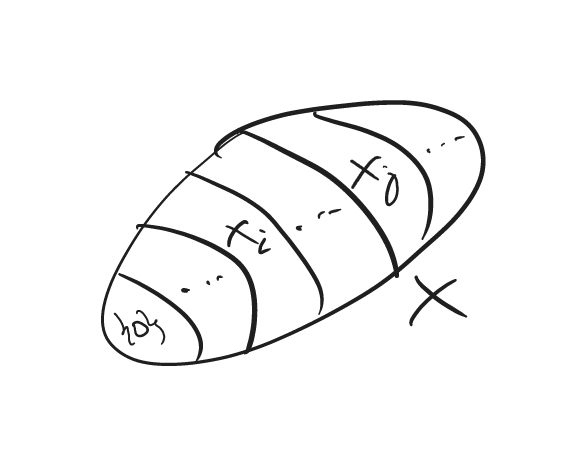
\includegraphics[width=0.5\textwidth]{set_x}
        \centering
    \end{figure}
    Без ограничения общности можно считать, что $X_i \subseteq X_j$, тогда $a, b \in X_j$. Так как $X_j$ -- подгруппа, то $a + b \in X_j$ и $-a \in X_j$. Следовательно, $a + b \in X$ и $-a \in X$, а значит $X$ -- подгруппа.
    
    Осталось показать, что $X \cap A = 0$. Пусть это не так. Тогда существует $x \in X \cap A$ такой, что $x \neq 0$. Это означает, что существует такой индекс $i \in I$, что $x \in X_i$. Раз так, то отсюда будет следовать, что $X_i \cap A \neq 0$ -- противоречие с условием. Таким образом, $X$ -- подгруппа и $X \cap A = 0$, следовательно $X$ -- мажоранта цепи $\Gamma$.

    Итак, мы показали, что для произвольной цепи в частично упорядоченном множестве $M$ существует мажоранта, а значит, по лемме Цорна, в множестве $M$ будет существовать максимальная подгруппа, имеющая нулевое пересечение с подгруппой $A$. Что и требовалось доказать.
\end{proof}

\begin{lemma} \label{efiopia}
    Пусть $G$ -- конечная группа, $A, B$ -- подгруппы в $G$. Тогда $$ |AB| = \frac{|A| \cdot |B|}{|A \cap B|}. $$
\end{lemma}
\begin{proof}
    Рассмотрим отображение $$\varphi: A \times B \rightarrow AB$$ действующее следующим образом: $$ \varphi((a, b)) \mapsto ab, $$ где $a \in A$, $b \in B$.
    Оценим в нём число элементов, которые будут <<склеиваться>> друг с другом: $$ ab = a'b', $$ где $a, a' \in A \ $, $b,b' \in B$. Умножим это равенство на ${a'}^{-1}$ слева и на $b^{-1}$ справа: $$ {a'}^{-1}a = b' b^{-1}. $$ Обозначим этот элемент как $c$. Нетрудно видеть, что он будет лежать в $A \cap B$.
    Из равенства ${a'}^{-1}a = c$ следует, что $a' = a c^{-1}$. Аналогично, из равенства $b' b^{-1} = c$ следует, что $b' = cb$.
    
    Таким образом мы получаем, что $\varphi((a, b)) = \varphi((ac^{-1}, cb))$, где $c \in A \cap B$. Нетрудно видеть, что для произвольной пары $(a, b)$ общее количество таких пар равно $|A \cap B|$. Или, что то же самое: для каждого элемента $ab \in AB$ существует ровно $|A \cap B|$ пар из $A \times B$, которые переходят в элемент $ab$ при отображении $\varphi$: $$ |AB| \cdot |A \cap B| = |A \times B|. $$ Отсюда получаем: $$ |AB| = \frac{|A| \cdot |B|}{|A \cap B|}, $$ что и требовалось доказать.
\end{proof}

\begin{lemma} \label{rafah}
    Пусть $G$ -- группа, $A \trianglelefteq G$, $B \leqslant G$. Тогда $AB \leqslant G$.
\end{lemma}
\begin{proof}
    Пусть $a_1 b_1, a_2 b_2 \in AB$, тогда:
    \[
        a_1 b_1 \cdot a_2 b_2 = a_1 \underbrace{b_1 a_2 b_1^{-1}}_{= a' \in A} \cdot b_1 b_2 = a_1 a' \cdot b_1 b_2 \in AB.
    \]
    Теперь посмотрим на обратный элемент: $ab \cdot b^{-1} a^{-1} = e$, тогда $$ b^{-1} a^{-1} = \underbrace{b^{-1} a^{-1} b}_{\in A} b^{-1} \in AB. $$
    Таким образом, $AB$ -- подгруппа в $G$.
\end{proof}

\begin{lemma} \label{eritrea}
    Если $A, B \triangleleft G$ и $A \cap B = \{ e \}$, то $AB \cong A \times B$.
\end{lemma}
\begin{proof}
    По лемме \ref{rafah} $AB \leqslant G$. Покажем, что $AB \triangleleft G$. Действительно, пусть $ab \in AB$ и $g \in G$, тогда:
    \[
        g^{-1} ab g = \underbrace{g^{-1} a g}_{\in A} \underbrace{g^{-1} b g}_{\in B} \in AB \Rightarrow AB \triangleleft G.
    \]

    Теперь покажем, что элемент из $AB$ представляется единственным образом. Пусть $ab, a'b' \in AB$ и $ab = a'b'$. Домножим слева на $a'^{-1}$ и справа на $b^{-1}$: $$ \underbrace{a'^{-1} a}_{\in A} = \underbrace{b' b^{-1}}_{\in B}. $$ Но так как $A \cap B = \{ e \}$, то $a'^{-1} a = b' b^{-1} = e \Rightarrow a' = a$ и $b' = b$.

    Теперь построим изоморфизм $\varphi: AB \rightarrow A \times B$ следующим образом: $$ \varphi(ab) = (a, b). $$
\end{proof}

\begin{theorem} \label{fhsuopi}
    Пересечение конечного числа подгрупп конечного индекса само имеет конечный индекс.
\end{theorem}
\begin{proof}
    Теорему достаточно доказать для случая двух подгрупп, и тогда по индукции она будет справедлива для любого конечного числа подгрупп.

    Пусть $G$ -- группа и $H_1, H_2$ -- её подгруппы конечного индекса, т.е. $|G: H_1| < \infty$ и $|G: H_2| < \infty$.
    Проведём оценку числа смежных классов группы $H_1$ по подгруппе $H_1 \cap H_2$ и группы $G$ по подгруппе $H_2$. Пусть $x, y \in H_1$ и $x(H_1 \cap H_2) \neq y(H_1 \cap H_2)$ -- различные смежные классы группы $H_1$ по подгруппе $H_1 \cap H_2$.
    Тогда $y^{-1} x (H_1 \cap H_2) \neq (H_1 \cap H_2)$, что означает $y^{-1} x \notin H_1 \cap H_2$. Так как $y^{-1} x \in H_1$, то $y^{-1} x \notin H_2$.
    Убедимся, что тогда $xH_2 \neq y H_2$. Действительно, пусть это не так и $x H_2 = y H_2$. Тогда $ y^{-1} x H_2 = H_2 \Rightarrow y^{-1} x \in H_2$ -- противоречие с тем, что $y^{-1} x \in H_1$ и $y^{-1} x \notin H_1 \cap H_2$.
    
    Получается, что число всевозможных комбинаций различных смежных классов группы $H_1$ по подгруппе $H_1 \cap H_2$ не превосходит числа всевозможных комбинаций различных смежных классов группы $G$ по подгруппе $H_2$. Действительно, если бы это было не так и $|H_1:H_1 \cap H_2|$ было бы бесконечно, то тогда и $|G:H_2|$ тоже -- противоречие с конечностью индекса подгруппы $H_2$. Поэтому получаем, что $$ |H_1:H_1 \cap H_2| \leqslant |G:H_2| < \infty. $$
\end{proof}

\begin{lemma} \label{pdenif}
    Если $G$ -- конечно порождённая группа и $H \trianglelefteq G$, то $G/H$ -- тоже конечно порождённая.
\end{lemma}
\begin{proof}
    Пусть $G = \{ g_1, g_2, \ldots g_k \mid g_j \in G \}$. Тогда нетрудно увидеть, что $$ G/H = \langle g_1 H, g_2 H, \ldots, g_k H \mid g_i \in G \rangle. $$
\end{proof}

\begin{lemma} \label{cvnmweo}
    $\mathbb{C}_n \cong \mathbb{Z}_n$
\end{lemma}
\begin{proof}
    Так как эти группы циклические, то пусть $a$ -- образующий группы $\mathbb{C}_n$ и $b$ -- образующий группы $\mathbb{Z}_n$, тогда построим отображение $\varphi: \mathbb{C}_n \rightarrow \mathbb{Z}_n$ следующим образом: $$ \varphi(a^k) = b^k. $$
    
    Убедимся, что $\varphi$ -- гомоморфизм. Действительно
    \begin{gather*}
        \varphi(xy) = \varphi(a^k a^m) = \varphi(a^{k + m}) = b^{k + m} = b^k b^m = \\
        = \varphi(a^k) \varphi(a^m) = \varphi(x) \varphi(y).
    \end{gather*}
    Таким образом, $\varphi$ -- гомоморфизм.

    Гомоморфизм $\varphi$, очевидно, сюръективен. Покажем, что он инъективен. Действительно, пусть $\varphi(x) = \varphi(y)$, тогда
    \begin{gather*}
        \varphi(a^k) = \varphi(a^m), \\
        b^k = b^m, \\
        \varphi^{-1}(b^k) = \varphi^{-1}(b^m), \\
        a^k = a^m \Rightarrow x = y.
    \end{gather*}
    Таким образом, $\varphi$ -- биективный гомоморфизм, а значит, является изоморфизмом между группами $\mathbb{C}_n$ и $\mathbb{Z}_n$ -- что и требовалось доказать.
\end{proof}

\begin{theorem}[Диксон] \label{djaios}
    Любая подгруппа конечного индекса содержит нормальную подгруппу конечного индекса.
    Более точно: если $H$ -- подгруппа индекса $k$ в $G$, то существует подгруппа $H_1 \triangleleft G$, $H_1 \leqslant H$ и $|G : H_1| \leqslant k!$
\end{theorem}
\begin{proof}
    Рассмотрим правое дествие группы $G$ на множестве правых смежных классов:
    \[
        G/H = \{ H a_1, H a_2, \ldots , H a_k \}.
    \]
    Заметим, что среди этого множества будет лежать $H$ в таком виде: $H a_t$, где $a_t \in H$ (то есть не в виде $H e$). 
    Действие группы будет определяться следующим образом:
    \[
        H a_i \cdot g = H a_j, \ g \in G.
    \]

    Заметим, что элемент $g \in G$ будет действовать на множестве $G/H$ как подстановка, потому что если $H a_i \neq H a_j$, то $H a_i g \neq H a_j g$.
    На основании этого факта определим отображение $\varphi: G \rightarrow \mathbf{S}_k$ и проверим, что это гомоморфизм.
    Пусть $g, h \in G$, $\varphi(g) = \sigma$, $\varphi(h) = \tau$ и $g,h$ действуют на $G/H$ следующим образом: $$ H a_i \xrightarrow{g} H a_j \xrightarrow{h} H a_t. $$
    Тогда
    \[
        i \xrightarrow{\sigma} j \xrightarrow{\tau} t.
    \]
    Отсюда видно, что $\varphi(gh) = \varphi(g) \varphi(h)$.

    Раз $\varphi: G \rightarrow \mathbf{S}_k$ -- гомоморфизм, то
    \[
        \faktor{G}{\textrm{ker} \ \varphi} \cong \textrm{im} \ \varphi \subseteq \mathbf{S}_k.
    \]
    Как известно, $\textrm{ker} \ \varphi$ -- нормальная подгруппа. Кроме того, $\textrm{ker} \ \varphi \subseteq H$. Действительно,
    \[
        \textrm{ker} \ \varphi = \{ g \in G \mid H a_i g = H a_i \text{ для } i=1,2,\ldots, k \}.
    \]
    Нетрудно заметить, что $G/H$ содержит такое $H a_i$, что $a_i \in H$ и $H a_i = H$. Далее, так как для всякого $g \in \textrm{ker} \ \varphi$ выполнено $H g = H$, то отсюда следует, что $g \in H \Rightarrow \textrm{ker} \ \varphi \subseteq H$.

    Наконец, так как $\varphi: G \rightarrow \mathbf{S}_k$, то $|\textrm{ker} \ \varphi| \leqslant k!$
\end{proof}

\subsection{Периодические группы}

Мощность $|G|$ группы $G$ называется \textit{порядком} группы. Если эта мощность конечна, то группа $G$ называется \textit{конечной}, в противном случае -- \textit{бесконечной}.

\textit{Порядком} элемента группы $g$ называется наименьшее $m > 0$ такое, что $g^m = e$ и обозначается $$ o(g) = m. $$

Группа называется \textit{периодической}, если все её елементы имеют конечный порядок.

Если порядки элементов периодической группы ограничены в совокупности, то их наименьшее общее кратное (НОК) называется \textit{периодом} или \textit{показателем} группы.

Приведём некоторые очевидные следствия из этих определений.

\begin{corollary}
    Если период группы существует, то это конечное число.
\end{corollary}

\begin{corollary}
    Все конечные группы являются периодическими.
\end{corollary}

\begin{proof}
    Так как порядок каждого элемента конечен, то НОК порядков всех элементов -- тоже конечное число.
\end{proof}

\begin{corollary}
    Существует периодическая группа, содержащая бесконечное число элементов.
\end{corollary}

\begin{proof}
Например это возможно, когда в группе есть бесконечно много элементов простого порядка $p$.
\end{proof}

\begin{lemma}
    Существует бесконечная несчётная периодическая группа конечного периода.
\end{lemma}
\begin{proof}
    Возьмём прямое произведение несчётного числа групп из двух элементов. Нетрудно убедиться, что тогда каждый элемент, возведённый в квадрат будет равен единице. Таким образом мы построили группу, обладающую несчётным числом элементов и у которой период равен двум. 
\end{proof}

Таким образом периодические группы можно разделить на два класса: конечные и бесконечные.

\begin{lemma} \label{nfi384}
    Пусть $G$ --  конечная группа, тогда порядок любого элемента делит порядок группы.
\end{lemma}
\begin{proof}
    Возьмём циклическую подгруппу, порождённую некоторым элементом из $G$. По теореме Лагранжа порядок подгруппы делит порядок группы, а раз подгруппа циклическая, то и порядок элемента делит порядок группы $G$.
\end{proof}

\begin{lemma}
    Пусть $G$ -- конечная группа. Если для некоторого $x \in G$ и простого $p$ верно, что $x^p = e$, то $o(x) = p$.
\end{lemma}
\begin{proof}
    Пусть это не так и существует такое $k < p$, что $o(x) = k$. Разделим $p$ на $k$: $$ p = kn + r, \ 0 \leqslant r < k. $$ Остаток $r$ не может быть равен нулю, так как $p$ -- простое, поэтому $0 < r < k$. Тогда: $$ x^p = x^{kn + r} = x^{kn} x^r = {\underbrace{(x^k)}_{=e}}^n x^r = x^r = e. $$ Получаем, что $x^r = e$, $r < k$, что противоречит минимальности $k$ -- противоречие. Следовательно $o(x) = p$.
\end{proof}

\begin{lemma} \label{fjoir}
        Если $G$ -- конечная группа, то для любого $x \in G$ верно: $$ x^{|G|} = e, $$ где $e$ -- единица группы $G$.
\end{lemma}
\begin{proof}
    По лемме \ref{nfi384} порядок любого элемента делит порядок группы, то есть существуют такие $n > 0, \ m > 0$ что $|G| = n m$ и $o(x) = n$. Тогда $$ x^{|G|} = x^{nm} = (x^n)^m = e^m = e. $$
\end{proof}

\begin{lemma}
    Показатель конечной группы $G$ является делителем её порядка.
\end{lemma}
\begin{proof}
    Так как по лемме \ref{nfi384} порядок каждого элемента делит порядок группы, то порядок группы должен быть числом, которое делится одновременно на все порядки элементов группы. Если среди таких чисел выбрать наименьшее, то оно будет в точности совпадать с наименьшим общим кратным порядков всех элементов группы, а значит, по определению -- с показателем группы: $$ |G| \geqslant \textrm{НОК}(\{o(x) \mid x \in G \}). $$
    Более точно можно записать так: $$ |G| = k \cdot \textrm{НОК}(\{o(x) \mid x \in G \}), $$ где $k > 0$. Таким образом получаем, что показатель группы делит порядок группы -- что и требовалось доказать.
\end{proof}

\begin{lemma} \label{dqiopnw}
    Пусть $G$ -- группа, тогда для любого $a \in G$
    \[
        a^m = e \Leftrightarrow (g^{-1} a g)^m = e, \ \forall g \in G.
    \]
\end{lemma}
\begin{proof}
    \textit{Необходимость.} Пусть выполнено, что $a^m = e$. Тогда осуществим ряд преобразований этого уравнения
    \begin{gather*}
        g^{-1} a^m g = g^{-1} g, \\
        g^{-1} \underbrace{a a \ldots a}_{m} g = e, \\
        \underbrace{(g^{-1} a g) (g^{-1} a g) \ldots (g^{-1} a g)}_{m} = e, \\
        (g^{-1} a g)^m = e.
    \end{gather*}

    \textit{Достаточность.} Пусть $(g^{-1} a g)^m = e$, тогда проделывая в обратном порядке те же преобразования, что и выше, мы и получаем, что $a^m = e$.
\end{proof}

\begin{lemma} \label{fenjoi}
    Пусть $G$ -- группа и $a \in G$, тогда
    \[
        o(a) = o(g^{-1} a g), \ \forall g \in G.
    \]
\end{lemma}
\begin{proof}
    Пусть $o(a) = m$, тогда по лемме \ref{dqiopnw} $(g^{-1} a g)^m = e$. Предположим, что число $m$ не является порядком сопряжённого элемента $g^{-1} a g$. Пусть $o(g^{-1} a g) = k$. Случай, когда $k > m$ невозможен, так как тогда $o(g^{-1} a g) = m$. Тогда пусть $k < m$. Но тогда по лемме \ref{dqiopnw} $a^k = e$, что противоречит минимальности $m$. Таким образом, $k = m$.
\end{proof}

\subsection{Полициклические группы}

Данный раздел сформирован на основе упражнения 4.4.3 (\cite{kargapolov}, с.56) и нужен для доказательства части б) теоремы \ref{equinor} (\cite{kargapolov}, с.158, теорема 17.2.2), но пока что леммы из этого раздела нигде не используются.

Напомним, что субнормальная матрёшка с циклическими секциями называется \textit{полициклической}, а группа с такой матрёшкой -- \textit{полициклической группой}.

\begin{lemma}
    Подгруппа полициклической группы полициклическая
\end{lemma}
\begin{proof}
    Пусть $G$ -- полициклическая группа и $H \leqslant G$. Раз $G$ -- полициклическая, то существует ряд
    \[
        G = G_0 > G_1 > G_2 > \ldots > G_k = \{ e\}
    \]
    с циклическими факторами.
    Построим ряд для подгруппы $H$:
    \[
        H \geqslant H \cap G_1 \geqslant H \cap G_2 \geqslant \ldots \geqslant H \cap G_k = \{ e \}
    \]
    и покажем, что все его факторы $ \faktor{H \cap G_i}{H \cap G_{i + 1}} $ тоже циклические. Действительно, по второй теореме об изоморфизме для всяких подгрупп $B, C$ некоторой группы $A$ таких, что $C \leqslant A$ и $B \trianglelefteq A$ имеем:
    \[
        \faktor{BC}{B} \cong \faktor{C}{B \cap C}.
    \]
    Заметим, что $BC$ будет являться подгруппой по лемме \ref{rafah}. Далее, обозначим $A = G_i$, $B = G_{i + 1}$ и $C = H \cap G_i$. Тогда, с учётом этих обозначений, а также того, что $G_{i + 1} \subset G_i \Rightarrow G_{i + 1} \cap G_i = G_{i + 1}$ получим:
    \begin{gather*}
        \faktor{H \cap G_i}{H \cap G_{i + 1}} = \faktor{C}{B \cap C} \cong \faktor{BC}{B} = \\
         = \faktor{G_{i + 1}(H \cap G_i)}{G_{i + 1}} \leqslant \faktor{G_i}{G_{i + 1}}.
    \end{gather*}
    Действительно, это выполнено, так как $ G_{i + 1}\underbrace{(H \cap G_i)}_{\in G_i} \in G_{i + 1} $ -- так как $G_{i + 1} \subset G_i$.

    Значит, $ \faktor{H \cap G_i}{H \cap G_{i + 1}} $ изоморфна подгруппе группы $\faktor{G_i}{G_{i + 1}}$, а она по условию циклическая, а всякая подгруппа циклической группы -- снова циклическая.
    Таким образом, $ \faktor{H \cap G_i}{H \cap G_{i + 1}} $ -- циклическая группа -- что и требовалось доказать.
\end{proof}

\begin{lemma}
    Фактор-группа полициклической группы полициклическая.
\end{lemma}
\begin{proof}
    Пусть $G$ -- полициклическая группа. Это значит, что она обладает субнормальным рядом с циклическими секциями:
    \[
        \{ e \} = G_0 \trianglelefteq G_1 \trianglelefteq G_2 \trianglelefteq \ldots \trianglelefteq G_n = G.
    \]
    Пусть $H \trianglelefteq G$ и рассмотрим ряд на фактор-группе $G / H$\footnote{Мы здесь действительно имеем право рассматривать произведение подгрупп $G_i H$, так как $H \trianglelefteq G$, $G_i \leqslant G$, следовательно по лемме \ref{rafah} оно является подгруппой в $G$.}:
    \[
        1 = \overline{G}_0 \leqslant \overline{G}_1 \leqslant \overline{G}_2 \leqslant \ldots \leqslant \overline{G}_n = G / H, \text{ где } \overline{G}_i = \faktor{G_i H}{H}.
    \]
    Покажем, что это субнормальный ряд с циклическими секциями. Для того, чтобы показать субнормальность нужно убедиться, что $\overline{G}_i \trianglelefteq \overline{G}_{i + 1}$. Проверим это. Пусть $\overline{g_i} \in \overline{G}_i$,  $\overline{g}_{i + 1} \in \overline{G}_{i + 1}$ и рассмотрим сопряжённый
    \[
        (\overline{g}_{i + 1})^{-1} \cdot \overline{g}_i \cdot \overline{g}_{i + 1}.    
    \]
    Так как $\overline{G}_i = G_i H / H$, то $\overline{g}_i = g_i h H = g_i H$, где $g_i \in G_i$. Аналогично $\overline{g}_{i + 1} = g_{i + 1} H$, где $g_{i + 1} \in G_{i + 1}$. С учётом этого и нормальности $H$ в $G$ получаем:
    \begin{gather*}
        (\overline{g}_{i + 1})^{-1} \cdot \overline{g}_i \cdot \overline{g}_{i + 1} = (g_{i + 1} H)^{-1} (g_i H) (g_{i + 1} H) = \\
        = \underbrace{g_{i + 1}^{-1} g_i g_{i + 1}}_{\in G_i} H \in G_i H / H = \overline{G}_i.
    \end{gather*}
    Итак, нормальность $\overline{G}_i$ в $\overline{G}_{i + 1}$ показана.

    Остаётся показать, что секции $\overline{G}_{i + 1} / \overline{G}_i$ циклические. Действительно, из теорем об изоморфизме(\cite{kargapolov}, с.49, теорема 4.2.3 и 4.2.4) получается:
    \begin{gather*}
        \faktor{\overline{G}_{i + 1}}{\overline{G}_i} = \faktor{\faktor{G_{i + 1}H}{H}}{\faktor{G_iH}{H}} \cong \faktor{G_{i + 1} H}{ G_i H} \cong \\
        \cong \faktor{G_{i + 1}}{G_i (G_{i+1} \cap H)} \cong \faktor{G_{i + 1} / G_i}{G_i / G_i (G_{i+1} \cap H)}.
    \end{gather*}
    Но это означает, что $\faktor{\overline{G}_{i + 1}}{\overline{G}_i}$ является гомоморфным образом группы $G_{i + 1} / G_i$, а гомоморфный образ циклической группы -- циклическая группа.
\end{proof}

\begin{lemma} \label{eftiq}
    Расширение полициклической группы посредством полициклической группы -- снова полициклическая группа.
\end{lemma}
\begin{proof}
    Пусть $B$ -- полициклическая группа и пусть $A$ -- её расширение посредством фактор-группы $A / B$. Так как $B$ -- полициклическая, то она обладает полициклическим рядом $$ B \triangleright B_1 \triangleright \ldots \triangleright \{ e \}. $$
    Так как расширение происходит при помощи полициклической группы $A / B$, то $$ A / B \triangleright A_1 / B \triangleright \ldots \triangleright A_{k - 1} / B \triangleright A_k / B = \{ e \}. $$
    Тогда получим объединённый ряд $$ A > A_1 > A_2 > \ldots > A_{k - 1} > B \triangleright B_1 \triangleright \ldots \triangleright \{ e \}. $$
    Так как $B \triangleleft A$, то очевидно, что $B \triangleleft A_1, \ B \triangleleft A_2, \ldots, B \triangleleft A_k$, поэтому:
    $$ A \triangleright A_1 \triangleright A_2 \triangleright \ldots \triangleright A_{k - 1} \triangleright B \triangleright B_1 \triangleright \ldots \triangleright \{ e \}. $$ То есть получили полициклическую матрёшку, а значит расширение -- полициклическая группа.
\end{proof}

\begin{lemma}
    Произведение двух полициклических нормальных подгрупп произвольной группы -- полициклическая подгруппа.
\end{lemma}
\begin{proof}
    Пусть $A, B$ -- полициклические группы и $A, B \triangleleft G$. Рассмотрим $AB$. Заметим, что $$ \faktor{AB}{A} \cong B. $$
    Отсюда можно увидеть, что группа $AB$ будет являться расширением полициклической группы $A$ при помощи полициклической группы $B$ (потому что $B$ изоморфно фактор-группе $AB / A$, а расширение как раз и проводится при помощи такой фактор-группы), а значит, по лемме \ref{eftiq} она будет являться полициклической группой.
\end{proof}

\newpage

\section{Периодические абелевы группы}

Говорят, что $G$ -- группа \textit{без кручения}, если любой её элемент имеет бесконечный порядок.

В произвольной абелевой группе $G$ совокупность $T(G)$ всех элементов конечного порядка образует подгруппу, которая называется \textit{периодической частью} группы $G$.

\begin{lemma}
    Пусть $G$ -- группа, тогда фактор-группа $\faktor{G}{T(G)}$ -- группа без кручения.
\end{lemma}
\begin{proof}
    Тот факт, что $\faktor{G}{T(G)}$ -- группа без кручения можно записать следующим образом: $$ T(\faktor{G}{T(G)}) = T(G). $$
    Проверим, что это действительно так. Пусть $$ a + T(G) \in T(\faktor{G}{T(G)}), \ a \in G. $$
    Так как элемент $a + T(G)$ принадлежит периодической части, то он имеет конченый порядок $n > 0$ и тогда
    \begin{align*}
        n(a + T(G)) &= \overline{0} = T(G), \\
        na + n T(G) & = T(G).
    \end{align*}
    Так как $T(G)$ -- подгруппа, то 
    \[
        n T(G) = \underbrace{T(G) + T(G) + \ldots + T(G)}_{n \text{ раз}} = T(G),
    \] поэтому:
    \[
        na + T(G) = T(G) \Rightarrow na \in T(G).
    \]
    Но это означает, что элемент $na$ имеет некоторый конечный порядок $m$:
    \[
        o(na) = m \Rightarrow m(na) = (mn)a = 0 \Rightarrow o(a) \leqslant mn \Rightarrow a \in T(G).
    \]
    Раз так, то $a + T(G) = T(G)$ и $T(\faktor{G}{T(G)}) = T(G)$.
\end{proof}

Следует заметить, что вообще периодическая часть не выделяется своим прямым слагаемым (в отличие от делимой части). Рассмотрим в качестве иллюстрации следующий
\begin{example}
    Пусть
    \[
        \overline{G} = \overline{\sum_{p}} \mathbb{Z}_p, \ \ G = \sum_{p} \mathbb{Z}_p
    \]
    (суммирование по всем простым $p$). Очевидно, $G$ -- периодическая часть в $\overline{G}$. Покажем, что $\faktor{\overline{G}}{G}$ -- полная группа и $G$ не выделяется в $\overline{G}$ прямым слагаемым.
\end{example}
\begin{proof}
    Докажем сначала полноту фактор-группы $\faktor{\overline{G}}{G}$. Пусть $n$ -- положительное целое число и $f \in \overline{G}$. Тогда $f$ устроен следующим образом:
    \begin{equation} \tag{*} \label{mx}
        f = (\underbrace{a_2}_{\in \mathbb{Z}_2}, \underbrace{a_3}_{\in \mathbb{Z}_3}, \underbrace{a_5}_{\in \mathbb{Z}_5}, \underbrace{a_7}_{\in \mathbb{Z}_7}, \underbrace{a_{11}}_{\in \mathbb{Z}_{11}}, \ldots),
    \end{equation}
    индексация элементов кортежа здесь идёт простыми числами. Попробуем понять, при каких условиях уравнение $nx = f$ будет иметь решение в $\overline{G}$.
    Заметим, что это будет выполняться только в тех элементах кортежа \eqref{mx}, номера которых будут строго превышать $n$. То есть, решение уравнения $nx = a_p \in \mathbb{Z}_p$ будет существовать только тогда, когда $p > n$. Это означает, что при различных $p > n$ в каждой из групп $\mathbb{Z}_p$ существует элемент $g_p$ с условием:
    \[
        n g_p = f(p).
    \]
    <<Обнулим>> начальную часть кортежа, то есть на тех позициях, номера которых $\leqslant n$ мы поставим нули. Делать это мы будем, используя следующие обозначения:
    \[
        g(p) = 
        \begin{cases}
          0 & \text{ при } p \leqslant n, \\
          g_p & \text{ при } p > n,
       \end{cases}
       \ \ \ \
        f'(p) = 
        \begin{cases}
          0 & \text{ при } p \leqslant n, \\
          f(p) & \text{ при } p > n.
       \end{cases}
    \]
    Отсюда видно, что тогда $ng = f'$. Но $fG = f'G$, так как видно, что $f$ может быть получен путём прибавления того самого <<выброшенного>> куска, а он содержит лишь конечное число ненулевых компонент, а именно такие элементы и составляют $G$. Раз так, то уравнение $nx = fG$ имеет решение в $\faktor{\overline{G}}{G}$.

    Теперь допустим, что $G$ разлагается в прямую сумму $\overline{G} = G \oplus H$. Так как $\faktor{\overline{G}}{G}$ делима и $\faktor{\overline{G}}{G} \simeq H$ (по лемме \ref{eto_basa}), то $H$ тоже будет полна. То есть, в подгруппе $H$ при произвольном $n$ должно иметь решение уравнение $nx = h, \ h \in H$. Но это не так, так как, например, если $h(p) \neq 0$, то это уравнение не может иметь решений при $n = p$. Полученное противоречие доказывает наше утверждение относительно $\overline{G}$.
\end{proof}

\subsection*{Примарные группы}

Группа, в которой порядок каждого элемента равен степени простого числа $p$ называется \textit{p-группой}: $$ A(p) = A_p = \{ x \mid o(x) = p^n, n \geqslant 0 \}. $$
Такие группы образуют класс \textit{примарных} групп для различных простых $p$.

% В периодической абелевой группе $G$ совокупность $A_p$ всех элементов, порядки которых есть степени фиксированного простого числа $p$ образует подгруппу. Очевидно, $A_p$ -- максимальная $p$-подгруппа в $G$; она называется \textit{примарной компонентой} группы $G$.

\begin{corollary}
    Существуют бесконечные примарные группы.
\end{corollary}

\begin{corollary}
    Примарная группа является периодической.
\end{corollary}

\begin{proof}
    В примарной группе порядок любого элемента конечен.
\end{proof}

\begin{corollary}
    Существуют примарные группы, которые не имеют конечного периода.
\end{corollary}

\begin{lemma} \label{prime_period}
    Если $A(p)$ -- примарная группа, то её период равен $$ \max\{ o(x) \mid x \in A(p) \} = p^{\max \{ \log_p{o(x)} \mid x \in A(p) \} }. $$
\end{lemma}

\begin{lemma}
    Если $G$ -- p-группа конечного периода $p$, то для любого $ g \in G $ верно: $o(g) = 1$ либо $o(g) = p$.
\end{lemma}

\begin{proof}
    Так как период группы равен наименьшему общему кратному порядков всех её элементов, то он должен делиться на порядок любого элемента группы. Но период группы - простое число, а оно делится только на себя и на единицу, откуда и вытекает условие леммы.
\end{proof}

\begin{theorem}[О разложении периодической группы в прямую сумму примарных компонент] \label{fiona}
    Пусть $A$ -- периодическая абелева группа. Тогда
    \begin{enumerate}
        \item A(p) -- подгруппа группы $A$;
        \item $$ A = \sum_p A(p); $$
        \item Если $$ A = \sum_p A'(p), $$ где $A'(p)$ -- группа, у которой все элементы имеют порядки, являющиеся степенями простого числа $p$, то $A'(p) = A(p)$.
    \end{enumerate}
\end{theorem}
\begin{proof}
    1. Возьмём $x, y \in A(p)$, тогда $p^m x = 0$ и $p^n y = 0$ для $m, n \in \mathbb{N}$. Обозначим $t = \max (m, n)$, тогда:
    $$ p^t (x + y) = p^t x + p^t y = 0 + 0 = 0 \Rightarrow x + y \in A(p). $$
    Теперь возьмём $x \in A(p)$ и рассмотрим порядок элемента $-x$. Известно, что $$ o(x) = o(-x), $$ а это и означает, что $-x \in A(p)$. Таким образом, $A(p)$ -- подгруппа группы $A$.

    2. Пусть $a \in A$. Тогда $o(a) = p_1^{\alpha_1} p_2^{\alpha_2} \ldots p_k^{\alpha_k} = n$.
    Рассмотрим систему чисел $\{ q_i = \frac{n}{p_i^{\alpha_i}} \}_{i = 1..k}$:
    \begin{align*}
        q_1 =& p_2^{\alpha_2} \ldots p_k^{\alpha_k}, \\
        q_2 =& p_1^{\alpha_1} p_3^{\alpha_3} \ldots p_k^{\alpha_k}, \\
        \vdots & \\
        q_k =& p_1^{\alpha_1} p_2^{\alpha_2} \ldots p_{k - 1}^{\alpha_{k - 1}}.
    \end{align*}
    У всех этих чисел не будет общего делителя (кроме 1), а значит, они все взаимно просты, т.е.:
    $$ (q_1, q_2, \ldots, q_k) = 1. $$
    Это означает, что можно записать соотношение Безу, то есть существуют $u_1, u_2, \ldots, u_k$ такие, что
    $$ q_1 u_1 + \ldots + q_k u_k = 1. $$ Домножим это равенство слева и справа на $a$:
    \[
        \underbrace{q_1 u_1 a}_{\in A(p_1)} + \underbrace{q_2 u_2 a}_{\in A(p_2)} \ldots + \underbrace{q_k u_k a}_{\in A(p_k)} = a,
    \]
    то есть $q_i u_i a \in A(p_i)$, так как $p_i (q_i u_i a) = 0 \Rightarrow o(q_i u_i a) = p_i$. Таким образом мы показали, что $a \in \sum_p A(p)$.
    
    Осталось доказать, что $\sum_p A(p)$ -- действительно прямая сумма. Иначе говоря нужно показать, что $A(p_i) \cap \sum_{j \neq i} A(p_j) = \{ 0 \}$.
    Пусть это не так. Это означает, что это пересечение непусто, т.е.
    \[
        \exists x \in A(p_i) \cap \sum_{j \neq i} A(p_j), \ x \neq 0.
    \]
    Тогда, так как $x \in \sum_{i \neq j} A(p_j)$, то
    $$ x = x_1 + x_2 + \ldots x_{i - 1} + x_{i + 1} + \ldots + x_k.\footnote{\text{То есть в этой сумме отсутствует $x_i$.}} $$
    Это означает, что
    \begin{equation*}
        \begin{cases}
            p_1^{\beta_1} x_1 = 0 \\
            \vdots \\
            p_{i - 1}^{\beta_{i - 1}} x_{i - 1} = 0 \\
            p_{i + 1}^{\beta_{i + 1}} x_{i + 1} = 0 \\
            \vdots \\
            p_k^{\beta_k} x_k = 0
        \end{cases}.
    \end{equation*}
    Откуда следует, что
    \[
        p_1^{\beta_1} \ldots p_{i - 1}^{\beta_{i - 1}} p_{i + 1}^{\beta_{i + 1}} \ldots p_k^{\beta_k} \underbrace{(x_1 + \ldots + x_{i - 1} + x_{i + 1} + \ldots + x_k)}_{x} = 0.
    \]
    Но, так как $x \in A(p_i) \Rightarrow p_i^{\beta_i} x = 0$, то получаем:
    \begin{equation*}
        \begin{cases}
            p_1^{\beta_1} \ldots p_{i - 1}^{\beta_{i - 1}} p_{i + 1}^{\beta_{i + 1}} \ldots p_k^{\beta_k} x = 0 \\
            p_i^{\beta_i} x = 0
        \end{cases}.
    \end{equation*}
    Так как $$ (p_1^{\beta_1} \ldots p_{i - 1}^{\beta_{i - 1}} p_{i + 1}^{\beta_{i + 1}} \ldots p_k^{\beta_k}, p_i^{\beta_i}) = 1, $$ то $x = 0$, а следовательно, сумма прямая.

    3. То, что $A'(p) \subseteq A(p)$ для всех $p$ -- очевидно. Покажем, что $A(p) \subseteq A'(p)$ для любого $p$. От противного -- предположим, что это не так. Тогда найдётся такое $p'$, что $A'(p') \subset A(p')$. Следовательно, будет существовать такой $0 \neq x \in A$, что $x \in A(p')$ и $x \notin A'(p')$. Раз $x$ не принадлежит своему прямому слагаемому $A'(p')$, то по условию его можно разложить: $$ x = x_1 + x_2 + \ldots + x_k, $$ где $0 \neq x_1 \in A'(p_1), 0 \neq x_2 \in A'(p_2), \ldots, 0 \neq x_k \in A'(p_k)$. В этом разложении существует компонента $x_i \in A'(p')$.
    Если $x_i = 0$, то получаем:
    \begin{gather*}
        p_1^{\alpha_1} x_1 = 0, \\
        p_2^{\alpha_2} x_2 = 0, \\
        \vdots \\
        p_k^{\alpha_k} x_k  = 0,
    \end{gather*}
    среди которых нет строчки $(p')^\beta x_i = 0$.
    Отсюда получаем, что: $$ p_1^{\alpha_1} \dots p_k^{\alpha_k} x = 0, $$ где среди $p_1^{\alpha_1} \dots p_k^{\alpha_k}$ отсутствует множитель $(p')^\beta$. С другой стороны, так как $x \in A(p')$, то $(p')^\beta x = 0$. Получаем, что $x$ аннулируется двумя взаимно простыми числами, а значит $x = 0$ -- противоречие, так как мы предполагали, что $x \neq 0$.
    
    Теперь, если $x_i \neq 0$, то $$ x = x_1 + \dots + x_i + \dots + x_k, $$ где $x_j \neq 0$ для всех $1 \leqslant j \leqslant k$. Перенесём $x_i$ в левую часть: $$ x - x_i = x_1 + \dots + x_{i - 1} + x_{i + 1} + \dots +x_k. $$ Так как $x_i \in A'(p')$ и $x \in A(p')$, то получаем, что элемент $x - x_i$ будет аннулироваться какой-то степенью $p'$ и это число будет взаимно простым с тем, которое аннулирует элементы справа, следовательно $x - x_i = 0$ и $x = x_i$. Следовательно, $x \in A'(p')$ -- противоречие с условием.
\end{proof}

Следующий ряд утверждений сформулирован на основе доказательства первой теоремы Прюфера (\cite{kargapolov}, с. 92)

\begin{theorem} \label{rfunqweiop}
    Абелева группа $G$ простого периода $p$ разлагается в прямую сумму циклических подгрупп: $$ G = \sum_{i \in I} \langle a_i \rangle, $$ где $a_i \in G$.
\end{theorem}

\begin{proof}[Доказательство №1 -- через линейное пространство]
    Представим абелеву группу простого периода $p$ как линейное пространство над полем из $p$ элементов и воспользуемся теоремой о разложимости линейного пространства в прямую сумму подпространств.

    В качестве множества векторов у нас будут выступать элементы группы $G$, а в качестве скаляров - элементы поля $GF(p) = \mathbb{Z}_p$. Умножение определим так: $$ u \cdot g = \underbrace{g + \dots + g}_{u \, \text{раз}} \in G, $$ где $g \in G$, $u \in \mathbb{Z}_p$. При таком определении все аксиомы линейного пространства будут выполнены. То есть абелева группа $G$ будет являться линейным пространством над полем $\mathbb{Z}_p$.
    
    \textit{Случай 1}. Данное линейное пространство конечномерно. Тогда в нём существует базис $\{ e_1, \dots, e_n \}$ и группа разлагается по нему: $$ G = \mathbb{Z}_p e_1 \oplus \ldots \oplus \mathbb{Z}_p e_n $$ как линейное пространство. При этом $$ \underbrace{\mathbb{Z}_p e_i}_{(0, \dots, 0, \star, 0, \dots, 0 )} \cap \underbrace{\sum_{j \neq i} \mathbb{Z}_p e_j}_{(\star, \dots, \star, 0, \star, \dots, \star )} = \{ 0 \}. $$

    \textit{Случай 2}. Линейное пространство бесконечномерно. Для того, чтобы применить теорему о разложимости на подпространства, нам нужно показать, что в данном линейном пространстве существует максимальное линейно независимое подмножество векторов, которое порождает всё пространство.

    Существование такого максимального линейно независимого подмножества будем доказывать при помощи леммы Цорна. Пусть $M$ -- множество всех линейно независимых подмножеств линейного пространства $G$ над полем $\mathbb{Z}_p$. Такие существуют -- например множество, состоящее из одного ненулевого элемента $\{ g \}$, $g \in G$ -- очевидно, что оно линейно независимо. Нетрудно заметить, что множество $M$ будет частично упорядоченным множеством по операции теоретико-множественного включения. Пусть $I$ -- произвольное множество индексов и $\Gamma = \{ X_\gamma \mid \gamma \in I \}$ -- произвольная цепь в $M$. Чтобы применить лемму Цорна нам нужно показать, что любая такая цепь имеет мажоранту. Рассмотрим множество $$ X = \bigcup_{i \in I} X_i $$ и проверим, будет ли оно являться мажорантой цепи $\Gamma$. То, что $X$ будет являться верхней гранью для любого элемента цепи $\Gamma$ очевидно. Остаётся показать, что $X \in M$, то есть что $X$ -- линейно независимое подмножество. Возьмём произвольные $ x_1, \dots, x_n \in X$ и рассмотрим линейную комбинацию $$ \lambda_1 x_1 + \lambda_2 x_2 + \ldots + \lambda_n x_n, $$ где $\lambda_i \in GF(p)$. Так как $\Gamma$ -- цепь, то для любых пар индексов $\alpha, \beta \in I$ выполняется $X_\alpha \subseteq X_\beta$ либо $X_\beta \subseteq X_\alpha$, а значит, существует такой индекс $\gamma \in I$, что $ x_1, \dots, x_n \in X_\gamma$, откуда следует, что $ \{ x_1, \dots , x_n \} $ -- линейно независимое подмножество. Таким образом, по лемме Цорна в $G$ существует максимальная линейно независимое подмножество.

    Покажем, что любой элемент из $x \in G$ выражается через это множество. Возможны два случая: $x \in X$ и $x \notin X$. Если $x \in X$, то он выражается через эту систему: $$ x = 1 \cdot x. $$ Пусть $x \notin X$, Так как $X$ -- максимальная линейно независимая система векторов, то $X \cup \{ x \}$ будет линейно зависима. Это значит, что $$ \lambda_1 x_1 + \ldots + \lambda_n x_n + \mu x = 0, $$ где $\lambda_1, \dots, \lambda_n, \mu$ не все нулевые.
    Рассмотрим два случая.
    \begin{enumerate}
        \item[(а)] $\mu  = 0 \Rightarrow \lambda_1 x_1 + \ldots + \lambda_n x_n = 0 $, а это возможно только при $\lambda_1 = \lambda_2 = \dots = \lambda_n = 0$, так как $x_1, \dots, x_n$ -- линейно независимая система векторов. Но мы же предполагали, что среди $\lambda_1, \dots, \lambda_n, \mu$ не все нулевые -- противоречие.
        \item[(б)] $\mu \neq 0$. Тогда $$ \lambda_1 x_1 + \ldots + \lambda_n x_n = - \mu x, $$ что означает, что $x$ раскладывается по $X$.
    \end{enumerate}

    Применяя теорему о разложимости линейного пространства в прямую сумму подпространств получаем разложение $G$ как линейного пространства над своим базисом $\{ e_\alpha \mid \alpha \in I \}$: $$ G = \bigoplus \sum_{\alpha \in I} \mathbb{Z}_p e_{\alpha}. $$ Откуда следует, что как абелева группа $G$ раскладывается в прямую сумму циклических подгрупп: $$ G = \bigoplus_{\alpha \in I} \mathbb{Z}_p. $$
\end{proof}
\begin{proof}[Доказательство №2 -- трансфинитной индукцией]
    Пусть $G \neq 0$ и рассмотрим подгруппу, порождённую каким-либо ненулевым элементом из $G$: $$ G_1 = \{ 0, a, 2a, \ldots, (p-1)a \}. $$
    Для каждого ординала $\xi$ строим $G_\xi$ следующим образом.

    \textit{Базис}: $\xi = 1$. Тогда $G_\xi$ уже построено.

    \textit{Индукционный шаг}. Пусть $\forall \eta < \xi$ группа $G_\eta$ построена. Тогда рассмотрим два случая:
    \begin{enumerate}
        \item[(а)] $\xi$ -- не предельный ординал. Тогда $\xi = \eta + 1$. Если $G_\eta  = G$, то $G_{\eta + 1} = G_\eta$ и всё доказано. Если же $G_\eta \neq G$, то берём $x \notin G_\eta$. Тогда $\langle x \rangle = \mathbb{Z}_p$, при этом $$ G_\eta \cap \langle x \rangle = 0. $$ Это действительно так, потому что пересечение подгрупп будет подгруппой, а все подгруппы группы $\langle x \rangle$ -- это $\{ 0 \}$ и $\langle x \rangle$. Но случай, когда $\langle x \rangle \subset G_\eta$ невозможен, так как мы выбрали $x \notin G_\eta$, следовательно, $G_\eta$ пересекается с $\langle x \rangle$ по нулю.
        Тогда в качестве $G_\xi = G_{\eta + 1}$ берём $G_\eta \oplus \langle x \rangle$, которое будет являться прямой суммой.

        \item[(б)] $\xi$ -- предельный ординал. Тогда положим: $$ G_\xi = \bigcup_{\eta < \xi}  G_\eta. $$
    \end{enumerate}

    Таким образом, для каждого ординала $\xi$ построена группа $G_\xi$, которая является прямой суммой групп, изоморфных $\mathbb{Z}_p$.
    Понятно, что $G_{\xi_1} \subseteq G_{\xi_2}$ при $\xi_1 < \xi_2$ (по построению).

    Берём ординал $\xi_0$, который по мощности больше, чем мощность $|G|$\footnote{Такой обязательно существует, так как по лемме Цермело любое множество можно вполне упорядочить. За каждым ординалом стоит какое-то вполне упорядоченное подмножество, а значит существуют ординалы, за которыми стоят подмножества более мощные, чем $|G|$. Тогда $G_{\xi_0}$ точно будет совпадать с $G_{\xi_0 + 1}$. Тут можно взять $2^{|G|}$, так как, например, если взять 40 подмножеств пятиэлементного множества, то среди них обязательно найдутся совпадающие. Более общо: если взять гиперконтинуум подмножеств, то среди них обязательно найдутся совпадающие, но в данном случае нам достаточно и $|G|$. Цепь, как набор подмножеств счётного множества не может быть несчётной.} и возьмём все такие $G_\xi$, где $\xi \leqslant \xi_0$. Все такие $G_\xi$ не могут быть различными, то есть существует такое $\eta$, что $$ G_\xi = G_\eta = G_{\eta + 1} = G_{\eta + 2} = \ldots $$ Таким образом мы исчерпаем все ординалы и $$ G_\xi = G. $$
\end{proof}

\begin{lemma}
    Пусть $G$ -- абелева p-группа с периодом $p^n$, $n > 0$. Тогда $pG = \{ pg \mid g \in G \}$ -- подгруппа группы $G$ с периодом $p^{n - 1}$.
\end{lemma}

\begin{proof}
    Сначала покажем, что $pG$ -- подгруппа группы $G$. Возьмём $ x, y \in pG $. По определению группы $pG$ это означает, что $x = px'$ и $y = py'$, где $x', y' \in G$. Тогда $$ x + y = px' + py' = p \underbrace{(x' + y')}_{ \in G} \in pG. $$
    Теперь, пусть $x \in pG$. Отсюда следует, что $x = px'$, где $x' \in G \Rightarrow  -x' \in G $, а значит $ p(-x') \in pG$. Следовательно, $pG$ -- подгруппа группы $G$.

    Теперь покажем, что период группы $pG$ равен $p^{n - 1}$. Пусть $g \in G$, тогда: $$ p^n g = 0 \Rightarrow p^{n - 1} (pg) = 0 \Rightarrow o(pg) = p^{n - 1}. $$
    А это и означает, что период группы $pG$ равен $p^{n - 1}$ и лемма доказана.

\end{proof}

\begin{lemma}
    Пусть $G$ -- абелева p-группа, у которой подгруппа $pG$ разлагается в прямую сумму циклических подгрупп: $$ pG = \sum_{i \in I} \langle a_i \rangle, $$ где $a_i \in pG$. Тогда уравнение $$ px = a_j $$ имеет решение в $G$ для любого $j \in I$.
\end{lemma}

\begin{proof}
    Возьмём $j \in I$ и рассмотрим прямую сумму циклических подгрупп $ \sum_{i \in I} \langle a_i \rangle $. В ней, очевидно, будет существовать элемент $$ 0 + \ldots + 0 + k a_j + 0 + \ldots + 0 \in \sum_{i \in I} \langle a_i \rangle, $$ где $k \in \mathbb{Z}$. В частности, элемент $$ 0 + \ldots + 0 + a_j + 0 + \ldots + 0 \in \sum_{i \in I} \langle a_i \rangle. $$ Следовательно, раз $ pG = \sum_{i \in I} \langle a_i \rangle $, то будет существовать такой элемент $pg \in pG$, что $$ pg =  0 + \ldots + 0 + a_j + 0 + \ldots + 0 = a_j, $$ что и требовалось доказать.
\end{proof}

\begin{lemma}
    Пусть $G$ -- абелева p-группа, у которой подгруппа $pG$ разлагается в прямую сумму циклических подгрупп: $$ pG = \sum_{i \in I} \langle a_i \rangle, $$ где $a_i \in pG$ и уравнение $$ px = a_j $$ имеет решение $x_j$ в $G$ для любого $j \in I$. Пусть $X = \{ x_i \mid i \in I \}$ -- подмножество решений уравнения $px = a_j$ в $G$. Положим $ H = \langle X \rangle $, тогда $$ H = \sum_{i \in I} \langle x_i \rangle. $$
\end{lemma}

\begin{proof}
    Ясно, что $H$ будет подгруппой в $G$ по построению.
    Сначала покажем, что $H \subseteq \sum_{i \in I} \langle x_i \rangle$. Возьмём $h \in H$, тогда существует его разложение по порождающему множеству $X$: 
    \begin{equation} \label{eq_h} \tag{$\star$}
        h = \varepsilon_1 a_1 + \varepsilon_2 a_2 + \ldots + \varepsilon_m a_m,
    \end{equation}
    где $\varepsilon_i = \pm 1$, $a_i \in X$, $ 0 < m < \infty $.
    Так как каждый $a_j$, $1 \leqslant j \leqslant m$ принимает значение какого-то элемента $x_i \in X$, то может случиться так, что для некоторых $1 \leqslant j,k \leqslant m$ будет верно, что: $$ a_j = a_k = x_i. $$ А это означает, что в разложении (\ref{eq_h}) можно сгруппировать те $a_k$, которые равны одному и тому же элементу порождающего множества $x_i$. Для того, чтобы сделать такую группировку, для каждого разложения (\ref{eq_h}) элемента $h \in H$ и каждого $i \in I$ (соответствует $x_i$ из порождающего множества) определим множество $$S_i = \{k \mid a_k = x_i, 1 \leqslant k \leqslant m \}.$$ То есть, множество $S_i$ содержит те индексы слагаемых в разложении (\ref{eq_h}), в которых $a_k = x_i$. Тогда разложение (\ref{eq_h}) в силу абелевости группы $G$ можно переписать так: $$ h = \underbrace{\underbrace{\left( \sum_{j \in S_1}{\varepsilon_j} \right) }_{\in \mathbb{Z}} x_{i_1}}_{\in \langle x_{i_1} \rangle} + \underbrace{\underbrace{\left( \sum_{j \in S_2}{\varepsilon_j} \right)}_{\in \mathbb{Z}} x_{i_2}}_{\in \langle x_{i_2} \rangle} + \ldots + \underbrace{\underbrace{\left( \sum_{j \in S_{l}}{\varepsilon_j} \right)}_{\in \mathbb{Z}} x_{i_l}}_{\in \langle x_{i_l} \rangle} \in \sum_{i \in I} \langle x_i \rangle, $$ где $\varepsilon_i = \pm 1$, $ i_1, i_2, \ldots, i_l \in I $, $l \leqslant m $ и $l$ равно числу различных $x_i$ в разложении (\ref{eq_h}). Что и требовалось доказать.

    Обратно, покажем, что $\sum_{i \in I} \langle x_i \rangle \subseteq H$. Возьмём $x \in \sum_{i \in I} \langle x_i \rangle$, тогда $$ x = k_{i_1} x_{i_1} + k_{i_2} x_{i_2} + \ldots + k_{i_l} x_{i_l}, $$ где $k_{i_j} \in \mathbb{Z}$, $i_1, i_2, \ldots, i_l \in I$, $l < \infty$ (так как сумма прямая). Тогда, в частности:
    \begin{multline*}
        x = \sgn (k_{i_1}) \underbrace{(1 + \ldots + 1)}_{k_{i_1} \text{раз}} x_{i_1} + \sgn (k_{i_2}) \underbrace{(1 + \ldots + 1)}_{k_{i_2} \text{раз}} x_{i_2} + \ldots \\
        \ldots + \sgn (k_{i_l}) \underbrace{(1 + \ldots + 1)}_{k_{i_l} \text{раз}} x_{i_l}.
    \end{multline*}
    Если раскрыть все скобки, то $x$ будет представим в виде: $$ x = \delta_1 a_1 + \delta_2 a_2 + \ldots + \delta_m a_m, $$ где $\delta_i = \pm 1$, $a_i \in \{x_{i_1}, \ldots, x_{i_l} \}, m = k_1 + k_2 + \ldots + k_l$. Следовательно, $x$ раскладывается по множеству порождающих $x_i$, и $x \in H$.

    Остаётся доказать, что $ \sum_{i \in I} \langle x_i \rangle $ -- прямая сумма. Возьмём $x \in \sum_{i \in I} \langle x_i \rangle $, тогда: $$ x = k_{i_1} x_{i_1} + k_{i_2} x_{i_2} + \ldots + k_{i_l} x_{i_l}, $$ где $i_1, \ldots, i_l \in I$, $k_{i_j} \in \mathbb{Z}$. Умножим обе части на $p$: $$ px = k_{i_1} p x_{i_1} + k_{i_2} p x_{i_2} + \ldots + k_{i_l} p x_{i_l}. $$ Так как каждое $x_{i_j}$ является решением уравнения $p x_{i_j} = a_{i_j}$ (по условию), то: $$ pG \ni px = k_{i_1} a_{i_1} + k_{i_2} a_{i_2} + \ldots + k_{i_l} a_{i_l} \in \sum_{i \in I} \langle a_i \rangle. $$ Так как из условия мы знаем, что $ pG = \sum_{i \in I} \langle a_i \rangle $ -- прямая сумма, то $ \sum_{i \in I} \langle x_i \rangle $ -- тоже будет являться прямой суммой. Что и требовалось доказать.
\end{proof}

\section{Теоремы Силова}

\subsection*{Сопряжённые элементы, нормальные подгруппы}

Говорят, что элемент группы $a$ \textit{сопряжён} с элементом $b$ посредством элемента $x$, если $$ a = x^{-1} b x. $$ Часто используют степенные обозначения: $$ x^{-1} b x = b^x. $$

\begin{lemma}
    $$ (ab)^x = a^x b^x, \, \, (a^x)^y = a^{xy}. $$
\end{lemma}
\begin{proof}
    $$ (ab)^x = x^{-1}abx = x^{-1}a x x^{-1} b x = a^x b^x, $$
    $$ (a^x)^y = y^{-1} a^x y = y^{-1} x^{-1} a x y = a^{xy}. $$
\end{proof}

Если $A, B$ -- два подмножества группы, то обозначают $$ A^B = \{ a^b \mid a\in A, b \in B \}. $$

\begin{lemma}
    Подгруппа $H$ группы $G$ тогда и только тогда нормальна в $G$, если $$ H^G \subseteq H. $$
\end{lemma}
\begin{proof}
    \textit{Необходимость}. Пусть $H$ -- нормальная подгруппа в $G$. Тогда рассмотрим множество $$ H^G = \{ h^g \mid h \in H, g \in G \} = \{ g^{-1} h g \mid h \in H, g \in G \}. $$ По определению нормальной подгруппы для всякого $g \in G$ выполняется $ gH=Hg $, что равносильно тому, что $g^{-1}Hg = H$. А это означает, что для всякого $h \in H$ $$g^{-1}hg \in H. $$ С учётом этого получаем, что каждый элемент из $H^G$ лежит  в $H$, а значит, $H^G \subseteq H$.

    \textit{Достаточность}. Пусть $H$ -- подгруппа в $G$ и выполняется $H^G \subseteq H$. Это означает, что для любых $h \in H$, $g \in G$ существует $h' \in H$ такое, что 
    \begin{equation} \label{eq_1}
        g^{-1} h g = h'.
    \end{equation}
    С одной стороны, умножая (\ref{eq_1}) на $g$ слева получаем: $$ hg = g h', $$ откуда следует, что
    \begin{equation} \label{eq_2}
        Hg \subseteq gH.
    \end{equation}
    С другой стороны, умножая (\ref{eq_1}) на $g^{-1}$ справа мы получим: $$ g^{-1} h = h' g^{-1}, $$ а следовательно, $g^{-1} H \subseteq H g^{-1}$. Так как $g^{-1} \in G$, то это равносильно $$ xH \subseteq Hx, $$ для всякого $x \in G$. Учитывая это, а также (\ref{eq_2}) заключаем, что $xH = Hx$ для любого $x \in G$, что и является критерием нормальности группы $H$. 
\end{proof}

\begin{lemma}
    Отображение группы $G$ на себя по правилу $$ a \mapsto a^x $$ (при фиксированном $x \in G$) является изоморфизмом.
\end{lemma}
\begin{proof}
    Обозначим данное в условии отображение группы $G$ на себя как $ \varphi_x: G \rightarrow G $, где $x \in G$. Сюръективность по условию, выполнена, а значит, нужно только проверить инъективность. Пусть $a, b \in G$ и $$\varphi_x (a) = \varphi_x(b).$$ Тогда $$ a^x = b^x \Leftrightarrow x^{-1} a x = x^{-1} b x.$$ Умножая на $x$ слева и на $x^{-1}$ справа получаем, что $a = b$. Следовательно, $\varphi_x$ -- изоморфизм для любого $x \in G$, что и требовалось доказать.
\end{proof}

\begin{lemma} \label{gachimuchi}
    Пусть $G$ --  группа и $a, b \in G$. Положим $a \sim b$, если $a$ и $b$ сопряжены в $G$. Тогда $\sim$ -- отношение эквивалентности.
\end{lemma}

\begin{proof}
    Сопряжённость элементов $a$ и $b$ в $G$ означает, что существует такой $x \in G$ что $a = b^x$. Проверим, будет ли являться это отношение отношением эквивалентности.
    
    \textit{Рефлексивность}. $$ a = a^x = x^{-1} a x. $$ Очевидно, это будет выполняться при $x = e$, где $e$ -- единица группы $G$.

    \textit{Симметричность}. Пусть $a \sim b$. Это означает, что $$ a = b^x \Rightarrow a = x^{-1} b x. $$ Умножив это уравнение на $x$ слева и на $x^{-1}$ справа получаем: $$ x a x^{-1} = b \Rightarrow b = a^{-x}.$$ Таким образом получаем, что $b \sim a$.
    
    \textit{Транзитивность}. Пусть $a \sim b$ и $b \sim c$. Это означает, что $$a = x^{-1} b x \text{ и } b = y^{-1} c y.$$ Подставляя второе уравнение в первое получаем: $$ a = x^{-1} y^{-1} c y x \Rightarrow a = c^{yx}. $$ Следовательно, $a \sim c$.
\end{proof}

С учётом доказанного выше получаем, что $G$ разбивается на непересекающиеся классы сопряжённых элементов $a^G$.

Подмножество $M^x$ называется \textit{сопряжённым} с подмножеством $M$ в группе $G$ при некотором $x \in G$. Нетрудно заметить, что $| M^x | = |M|$, а между собой эти множества могут как пересекаться, так и нет.

В отличие от смежных классов классы сопряжённых элементов не всегда равномощны. При вычислении их мощностей решающую роль играет понятие нормализатора. Пусть $M$ -- подмножество, $H$ -- подгруппа группы $G$. \textit{Нормализатором} множества $M$ в подгруппе $H$ называется множество $$ N_H(M) = \{ h \mid h \in H, M^h = M \}, $$ которое, как легко проверить, является подгруппой в $H$. Если не указано, в какой подгруппе $H$ берётся нормализатор, то это означает, что он берётся во всей группе $G$.

\begin{lemma}
    Если $M$ -- подмножество, $H$ -- подгруппа группы $G$, то нормализатор $N_H(M)$ является подгруппой группы $H$:
    \[
        N_H(M) \leqslant H.
    \]
\end{lemma}
\begin{proof}
    Пусть $a, b \in N_H(M)$. Тогда, по определению нормализатора, $a, b \in H$ и $$ M^a = M \text{ и } M^b = M. $$ Это означает, что $$ a^{-1} M a = M, \ b^{-1} M b = M. $$ Подставляя первое уравнение во второе получаем: $$ b^{-1} a^{-1} M a b = (ab)^{-1} M (ab) = M, $$ откуда следует, что $M^{ab} = M$. Так как $ab \in H$ (так как $H$ -- подгруппа), то получаем, что $ ab \in N_H(M)$.

    Теперь пусть $a \in N_H(M)$. Тогда $a \in H$ и $M^a = M$. Это означает, что $$ a^{-1} M a = M. $$ Умножим это равенство слева на $a$, а справа на $a^{-1}$: $$ M = a M a^{-1} = (a^{-1})^{-1} M a^{-1}. $$ Отсюда следует, что $M^{a^{-1}} = M$. Так как $a^{-1} \in H$ (так как $H$ -- подгруппа), то $a^{-1} \in N_H(M)$.
    Таким образом получили, что $N_H(M) \leqslant H$ -- что и требовалось доказать.
\end{proof}

\begin{lemma}
    Пусть $G$ -- группа. Подгруппа $H$ нормальна в $G$ тогда и только тогда, когда её нормализатор совпадает со всей группой: $$ N_G (H) = G. $$ 
\end{lemma}
\begin{proof}
    Пусть $H \trianglelefteq G$. Построим нормализатор подгруппы $H$:
    \[ \label{eq} \tag{$\ast$}
        N_G(H) = \{ g \in G \mid H^g = H \}.
    \]
    Таким образом, нам нужно показать, что $N_G(H) = G$. Включение $N_G (H) \subseteq G$ очевидно.

    Пусть $g \in G$. Так как $H$ -- нормальная, то $g^{-1} H g = H$. Но, именно такие элементы и составляют нормализатор \eqref{eq}, поэтому $g \in N_G(H) \Rightarrow G \subseteq N_G(H)$ и $N_G(H) = G$.

    Обратно, пусть $N_G(H) = G$. Тогда, по определению, $G$ состоит из элементов вида \eqref{eq}. То есть, для каждого $g \in G$ выполняется $ g^{-1} H g = H $, что и является критерием нормальности подгруппы $H$.
\end{proof}

Пусть $M$ -- подмножество, $H$ -- подгруппа группы $G$. Мы назвали нормализатором $M$ в $H$ совокупность тех элементов из $H$, которые перестановочны с множеством $M$ в целом. Можно рассмотреть также множество тех элементов из $H$, которые перестановочны с $M$ поэлементно, т.е.
\[
    C_H(M) = \{ h \in H \mid m^h = m \text{ для всех } m \in M \}.
\]
Это множество называется \textit{централизатором} множества $M$ в $H$ и является, как мы сейчас увидим, нормальной подгруппой нормализатора $N_H(M)$. Если не указано, в какой подгруппе $H$ берётся централизатор, то это означает, что он берётся во всей группе $G$.

\begin{lemma} \label{vweqwqw}
    Пусть $M$ -- подмножество, $H$ -- подгруппа группы $G$, тогда $$ C_H(M) \trianglelefteq N_H(M). $$
\end{lemma}
\begin{proof}
    Сначала убедимся, что $C_H(M)$ -- подгруппа в $N_H(M)$. То, что $C_H(M) \subseteq N_H(M)$ очевидно. Проверим, что это группа. Пусть $a, b \in C_H(M)$. Тогда для любого $m \in M$ выполняется, что $$ m^a = m \text{ и } m^b = m. $$ Или, что то же самое: $$ a^{-1} m a = m, \ b^{-1} m b = m. $$ Подставим первое равенство в левую часть второго: $$ b^{-1} a^{-1} m a b = m. $$ Откуда следует, что $m^{ab} = m$. Так как $a,b \in H$ и $m^{ab} = m$ получаем, что $ab \in C_H(M)$.
    Теперь пусть $a \in C_H(M)$. Так как $m^a = m$, то $$ a^{-1} m a = m. $$ Умножив это равенство слева на $a$ и справа на $a^{-1}$ получаем: $$ m = a m a^{-1}, $$ откуда следует, что $m^{a^{-1}} = m$. С учётом того, что $a^{-1} \in H$ получаем, что $a^{-1} \in C_H(M)$. Таким образом мы показали, что $C_H(M)$ -- подгруппа группы $N_H(M)$.

    Теперь покажем, что $C_H(M)$ является нормальной подгруппой группы $N_H(M)$, то есть для каждого $g \in N_H(M)$ должно выполняться $$ g^{-1} C_H(M) g \subseteq C_H(M). $$ Пусть $x \in g^{-1} C_H(M) g \Rightarrow x = g^{-1} h g$, где $h \in H$ такой, что $m^h = m$ для всякого $m \in M$. Тогда 
    \[
        m^x = m^{g^{-1} h g} = (g^{-1} h g)^{-1} m (g^{-1} h g) = g^{-1} h^{-1} \underbrace{g m g^{-1}}_{m^{g^{-1}}} h g = g^{-1} (m^{g^{-1}})^h g.
    \]
    Так как $g^{-1}\in N_H(M)$, то $m^{g^{-1}} \in M$. А раз $m^h = h$ для всех $m \in M$, то $(m^{g^{-1}})^h = m^{g^{-1}}$:
    $$
        g^{-1} (m^{g^{-1}})^h g = g^{-1} m^{g^{-1}} g = g^{-1} g m g^{-1} g = m.
    $$
    Таким образом мы получили, что $m^x = m$ для всякого $x \in g^{-1} C_H(M) g$. Учитывая это, а также то, что $x \in H$ (так как $x = g^{-1} h g$, где $g, g^{-1}, h \in H$) получаем, что $x \in C_H(M)$. Следовательно, подгруппа $C_H(M)$ нормальна в $N_H(M)$ -- что и требовалось доказать.
\end{proof}

Централизатор всей группы называется её \textit{центром} и обозначается $Z(G) = C_G(G)$. Так как $$ C_G(G) = \{ z \in G \mid g^{z} = g \text{ для всех } g \in G \}, $$ то рассмотрим $$ g^z = g \Rightarrow z^{-1} g z = g. $$ Умножим слева на $z$: $$ gz = zg. $$ То есть центр группы -- это множество таких элементов группы, которые коммутируют со всеми остальными её элементами. Таким образом можно считать, что $$ Z(G) = \{ z \in G \mid zg = gz \text{ для каждого } g \in G \}. $$ Группа тогда и только тогда абелева, когда она совпадает со своим центром. Единица всегда лежит в центре. Если других центральных элементов группа не содержит, то она называется \textit{группой с тривиальным центром} или \textit{группой без центра}

\begin{lemma}
    Пусть $G$ -- группа, тогда $$ Z(G) \trianglelefteq G. $$
\end{lemma}
\begin{proof}
    Проверим, что $Z(G)$ -- подгруппа. То, что $Z(G) \subseteq G$ очевидно. Пусть $a, b \in Z(G)$. Тогда $$ag = ga \text{ и } bg = gb$$ для любого $g \in G$. Умножим первое равенство справа на $b$: $$ agb = gab. $$ Теперь подставим второе равенство в левую часть последнего: $$ (ab)g = g(ab) \Rightarrow ab \in Z(G). $$
    Теперь пусть $a \in Z(G)$ и покажем, что $a^{-1} \in Z(G)$. Для каждого $g \in G$ имеем: $$ ag = ga. $$ Умножим слева и справа на $a^{-1}$: $$ a^{-1} (ag) a^{-1} = a^{-1} (ga) a^{-1} \Rightarrow g a^{-1} = a^{-1} g. $$ Таким образом $a^{-1} \in Z(G)$.

    Теперь покажем, что $Z(G)$ -- нормальная, а именно покажем, что $ g^{-1} Z(G) g \subseteq Z(G) $. Действительно, пусть $x \in g^{-1} Z(G) g \Rightarrow x = g^{-1} z g$ для некоторого $z \in Z(G)$. Но, так как $z$ коммутирует со всеми элементами группы, получаем: $$ x = g^{-1} z g = z g^{-1} g = z. $$ Раз $z \in Z(G)$, то и $x \in Z(G)$. Таким образом, $ g^{-1} Z(G) g \subseteq Z(G) $, а следовательно $Z(G)$ -- нормальная подгруппа в $G$, что и требовалось доказать.
\end{proof}

\begin{lemma}
    Если факторгруппа $G/Z(G)$ циклическая, то $G$ является абелевой.
\end{lemma}
\begin{proof}
    Рассмотрим естественный гомоморфизм $$ \varphi: G \rightarrow \faktor{G}{Z(G)}. $$ Так как любая циклическая группа абелева, то $$ \varphi(x) \varphi(y) = \varphi(y) \varphi(x), $$ где $x,y \in G$. По определению гомоморфизма $\varphi(xy) = \varphi(x) \varphi(y)$. С учётом этого получаем $$ xy = yx. $$ Что и требовалось доказать.
\end{proof}

\begin{lemma}
    Пусть $G$ -- группа, тогда центр является пересечением централизаторов всех элементов группы $G$: $$ Z(G) = \bigcap_{g \in G} C_G(g). $$
\end{lemma}
\begin{proof}
    Пусть $x \in \bigcap_{g \in G} C_G(g)$. Тогда, по определению централизатора: $$ x\in C_G(g) = \{ z \mid z \in G, g^z = g \} $$ для каждого $g \in G$. То есть для $x$ выполняется, что $g^x = g$. Но это означает, по определению: $$ x^{-1} g x = g \Rightarrow gx = xg. $$ Но именно такие $x$ и содержит центр группы, поэтому $x \in Z(G)$.

    Теперь пусть $x \in Z(G)$. Это означает, что $xg = gx$ для любого $g \in G$. Умножим слева на $x^{-1}$: $$ g = x^{-1} g x \Rightarrow g^x = g. $$ Отсюда видно, что $x \in C_G(g)$. Но, так как это выполнено для каждого $g \in G$, то отсюда следует, что $x \in \bigcap_{g \in G} C_G(g)$.

    Таким образом получили, что $  Z(G) = \bigcap_{g \in G} C_G(g) $ -- что и требовалось доказать.
\end{proof}

\subsection*{Действие группы на множестве}

Говорят, что группа $G$ \textit{действует на множестве} $M$, если для каждого элемента $m \in M$ и $g \in G$ определён элемент $mg \in M$, причём $$ (m g_1) g_2 = m(g_1 g_2) \text{ и } me = m, $$ для всех $m \in M$, $g_1, g_2 \in G$, $e$ -- единица группы $G$. Множество $$ mG = \{ mg \mid g \in G \} $$ называется \textit{орбитой} элемента $m$.

\begin{lemma}
    Пусть группа $G$ действует на множестве $M$. Если $m_1, m_2 \in M$ и $m_1 G \cap m_2 G  \neq \emptyset$, то $$ m_1 G = m_2 G. $$
\end{lemma}

\begin{proof}
    Если это так, то существуют такие $g_1, g_2 \in G$, что $$ m_1 g_1 = m_2 g_2. $$
    Умножим справа на $g_2^{-1} h$, где $h$ -- произвольный из $G$: $$ m_1 g_1 g_2^{-1} h = m_2 h. $$ Заметив, что $g_1 g_2^{-1} h \in G$ и что $h \in G$, получаем, что: $$ m_1 G = m_2 G. $$ Что и требовалось доказать.
\end{proof}

Отсюда заключаем, что орбиты двух элементов либо совпадают, либо не пересекаются.

Пусть группа $G$ действует на множестве $M$. \textit{Стабилизатором} элемента $m \in M$ называется множество $$ G_m = \{ g \mid g \in G, mg = m \}. $$

\begin{lemma}
    Пусть группа $G$ действует на множестве $M$, тогда для любого $m \in M$ множество $G_m$ является подгруппой в $G$.
\end{lemma}
\begin{proof}
    Пусть $m \in M$ и $a, b \in G_m$. Это значит, что $ma = m$ и $mb = m$. Подставим первое уравнение в левую часть второго: $$ (ma)b = m \Rightarrow m(ab) = m \Rightarrow ab \in G_m. $$

    Теперь пусть $a \in G_m$. Следовательно, $ma = m$. Умножая справа на $a^{-1}$ получаем: $m = m a^{-1} \Rightarrow a^{-1} \in G_m.$
    
    Таким образом, с учётом того, что $G_m \subseteq G$ получаем, что $G_m$ -- подгруппа в $G$, что и требовалось доказать. 
\end{proof}

\begin{lemma} \label{zfdsa}
    Пусть группа $G$ действует на множестве $M$, $m \in M$. Элементы $x, y \in G$ лежат в одном смежном классе по $G_m$ тогда и только тогда, когда $mx = my$.
\end{lemma}
\begin{proof}
    \textit{Необходимость}. Пусть $x, y$ лежать в одном смежном классе по подгруппе $G_m$. Это означает, что существует такой $h \in G$, что $x, y \in G_m h$. Значит, существуют такие $g_1, g_2 \in G_m$, что $x = g_1 h$, $y = g_2 h$ и $m g_1 = m$, $m g_2 = m$ для любого $m \in M$.
    Действуя элементом $m$ на $x$ и $y$ получаем:
    \begin{gather*}
        mx = mg_1 h, \ my = mg_2 h \Rightarrow \\
        \Rightarrow mx = mh, \ my = mh.
    \end{gather*}
    Следовательно, $mx = my$.

    \textit{Достаточность}. Пусть $mx = my$, $m \in M$. Возьмём подгруппу $G_m$ и рассмотрим правые смежные классы $G_m x$ и $G_m y$. Нужно показать, что $x$ и $y$ лежат в одном смежном классе, а так как смежные классы либо не пересекаются, либо совпадают, то достаточно доказать, что $G_m x = G_m y$.
    Докажем, что $G_m x \subseteq G_m y$. Пусть $g x \in G_m x$, где $g \in G_m$ такой, что $m g = m$, тогда: $$ g x = g x y^{-1} y. $$ Проверим, будет ли элемент $g x y^{-1}$ лежать в $G_m$, для этого подействуем на него элементом $m$: $$ m g x y^{-1} = m x y^{-1} = m y y^{-1} = m. $$ Таким образом, $g x y^{-1} \in G_m$, а значит $$ g x = \underbrace{g x y^{-1}}_{\in G_m} y \in G_m y. $$

    Случай $G_m y \subseteq G_m x$ разбирается аналогично. Получаем, что $G_m x = G_m y$, а значит, $x$ и $y$ лежат в одном смежном классе -- что и требовалось доказать.
\end{proof}

\begin{lemma}
    Пусть группа $G$ действует на множестве $M$, $m \in M$. Тогда отображение
    \begin{gather*}
        \varphi: \faktor{G}{G_m} \rightarrow mG,  \\
        \varphi(G_m x) = m x, \ x \in G
    \end{gather*}
    является биекцией.
\end{lemma}
\begin{proof}
    \textit{Инъективность}. Пусть $\varphi(G_m x) = \varphi(G_m y), \ x, y \in G$. Тогда $mx = my$. По лемме \ref{zfdsa} это означает, что $x, y$ лежат в одном смежном классе, а значит, $G_m x = G_m y$.

    \textit{Сюръективность}. Какой бы элемент из $mG$ мы не взяли, скажем $mx$, $x \in G$, его прообразом будет являться смежный класс $G_m x$. Следовательно, отображение $\varphi$ сюръективно.

    Таким образом мы получили, что отображение $\varphi$ является биекцией -- что и требовалось доказать.
\end{proof}

\begin{corollary}
    Если $G$ -- группа, действующая на множестве $M$ и $m \in M$, то порядок (или длина) орбиты $mG$ равна индексу стабилизатора элемента $m$: $$ |mG| = |G:G_m|. $$
\end{corollary}

Следующие утверждения сформулированы на основе доказательства теорем Силова (\cite{kargapolov}, с. 99).

\begin{lemma} \label{txdd}
    Пусть $G$ -- конечная группа, $|G| = n$ и $ \mathfrak{M} $ -- множество всех подмножеств мощности $k < n$ из $G$. Тогда для всякого $M \in \mathfrak{M}$ и $g \in G$ верно, что $$ Mg \in \mathfrak{M}. $$
\end{lemma}
\begin{proof}
    Переформулируем условие так: нужно показать, что $|Mg| = |M|$. Очевидно, что $|Mg| \leqslant |M|$. То есть, мощность множества $Mg$ не может возрасти относительно $M$. Предположим, что $|Mg| < |M|$. Тогда будут существовать $m_1, m_2 \in M$, $m_1 \neq m_2$ такие, что $$ m_1 g = m_2 g. $$ Умножив справа на $g^{-1}$ получим: $$ m_1 = m_2. $$ Получили противоречие, следовательно, $|Mg| = |M|$ и $Mg \in \mathfrak{M}$. 
\end{proof}

\begin{lemma} \label{zpre}
    Пусть $G$ -- конечная группа, $|G| = n$ и $ \mathfrak{M} $ -- множество всех подмножеств мощности $k < n$ из $G$. Пусть $\{ M_1, \dots , M_s \}$ -- орбита некоторого $M \in \mathfrak{M}$. Положим $$ G_i = \{ g \mid g \in G, M_1 g = M_i \}, $$ где $1 \leqslant i \leqslant s $. Тогда $G_1$ -- подгруппа в $G$, а $G_i$ -- в точности правые смежные классы группы $G$ по подгруппе $G_1$.
\end{lemma}

\begin{proof}
    Покажем, что $G_1$ -- подгруппа в $G$. Пусть $a, b \in G_1$. Тогда $M_1 a = M_1$ и $M_1 b = M_1$. Подставив первое уравнение во второе получим: $$ (M_1 a) b = M_1 \Rightarrow M_1(ab) = M_1 \Rightarrow ab \in G_1. $$
    Теперь покажем, что $a^{-1} \in G_1$. Пусть $a \in G_1$, тогда $$ M_1 a = M_1 \Leftrightarrow M_1 a a^{-1} = M_1 a^{-1} \Leftrightarrow M_1 = M_1 a^{-1} \Rightarrow a^{-1} \in G. $$

    Осталось показать, что $G_i$ -- в точности правые смежные классы группы $G$ по подгруппе $G_1$. Для начала заметим, что $$ G = G_1 \cup G_2 \cup \ldots \cup G_s. $$ Действительно, возьмём произвольный $g \in G$. Тогда будет существовать некоторый номер $i$ такой, что $M_1 g = M_i$ (так как $M_1$ -- элемент орбиты $MG$). Отсюда следует, что $g \in G_i$. То есть каждый $g \in G$ принадлежит какому-то $G_i$. Тогда, с учётом этого нам нужно показать, что $G_1 g_i = G_i$, где $\ g_i \in G_i$.
    
    Возьмём произвольный $g_i \in G_i$ и рассмотрим правый смежный класс $G_1 g_i$. Мы знаем, что $M_1 g_1 = M_1$ и $M_1 g_i = M_i$, при $g_1 \in G_1$. Тогда $$ M_1 g_1 g_i = M_1 g_i \Rightarrow M_1 g_1 g_i = M_i, $$ а это означает, что $g_1 g_i \in G_i \Rightarrow G_1 g_i \subseteq G_i$.
    Осталось показать, что $G_i \subseteq G_1 g_i$. Пусть $x \in G_i$. Тогда $M_1 x = M_i$. Учитывая, что $M_1 g_i = M_i$ получаем, что $$ M_1 x = M_1 g_i. $$ Умножим на $g_i^{-1}$ справа: $$ M_1 x g_i^{-1} = M_1, $$ откуда следует, что $$x g_i^{-1} \in G_1 \Rightarrow x g_i^{-1} g_i \in G_1 g_i \Rightarrow x \in G_1 g_i. $$ Таким образом получили, что $G_1 g_i = G_i$ для каждого $i \in \{ 1, \ldots, s\} $ -- что и требовалось доказать.
\end{proof}

\begin{lemma} \label{qxbn}
    Пусть $H$ -- подгруппа в $G$. Тогда $H^g$ -- подгруппа для любого $g \in G$.
\end{lemma}
\begin{proof}
    Пусть $g \in G$ и $a, b \in H^g = g^{-1} H g $. Тогда существуют такие $h_1, h_2 \in H$ что $$ a = g^{-1} h_1 g, \ b = g^{-1} h_2 g. $$ Тогда $$ ab =  g^{-1} h_1 g g^{-1} h_2 g = g^{-1} \underbrace{h_1 h_2}_{\in H} g \in H^g. $$ Теперь пусть $a \in H^g$. Тогда $a = g^{-1} h g$ для некоторого $h \in H$. Тогда $$ a^{-1} = (g^{-1} h g)^{-1} = g^{-1} \underbrace{h^{-1}}_{\in H} g \in H^g. $$
    Таким образом $H^g$ -- подгруппа группы $G$, что и требовалось доказать.
\end{proof}

\begin{lemma} \label{mtqr}
    Пусть $H$ -- подгруппа группы $G$. Тогда $H$ -- нормальная подгруппа в $N_G(H)$:
    \[
        H \trianglelefteq N_G(H).
    \]
\end{lemma}
\begin{proof}
    Сначала покажем, что $H$ -- подгруппа в $N_G(H)$. Для этого достаточно убедиться, что $H \subseteq N_G(H)$. Действительно, так как $$ N_G(H) = \{ g \mid g \in G, H^g = H \}, $$ то для любого $h \in H$ верно, что $H^h = h^{-1}Hh = H$, так как $H$ -- подгруппа. А значит, $h \in N_G(H) \Rightarrow H \subseteq N_G(H)$.

    Теперь убедимся, что $H \trianglelefteq N_G(H) $. Для этого проверим, что $g^{-1} H g \subseteq H$ для всякого $g \in N_G(H)$. Пусть $x \in g^{-1} H g$. Тогда существует такой $h \in H$, что $$ x = g^{-1} h g. $$ Из определения множества $N_G(H)$ следует что $H^g = H \Rightarrow g^{-1} H g = H \Rightarrow Hg = gH$. А это означает, что существует такой $h' \in H$, что $$ x = g^{-1} g h' = h' \in H. $$
    То есть мы получили, что если $x \in g^{-1} H g$, то $x \in H$. Следовательно, $H$ -- нормальная подгруппа в $N_G(H)$, что и требовалось доказать.
\end{proof}

\begin{lemma} \label{rafik}
    Пусть группа $G$ действует на себе посредством сопряжений. Элемент $g \in G$ лежит в центре $Z(G)$ тогда и только тогда, когда его класс сопряжённости состоит из единственного элемента: $$ x^G = \{ x \}. $$
\end{lemma}
\begin{proof}
    \textit{Необходимость}. Пусть $x \in Z(G)$, тогда класс сопряжённости элемента $x$: $$ x^G = \{ x^g \mid g \in G \} = \{ g^{-1} x g \mid g \in G \}.$$ Так как для любого $g \in G$ верно, что $xg = gx$, то получаем $$ x^G = \{ g^{-1} g x \mid g \in G \} = \{ x \mid g \in G \} = \{ x \}. $$

    \textit{Достаточность}. Пусть класс сопряжённости элемента $x$ состоит из одного элемента: $x^G = \{ x \}$. Это означает, что для всех $g \in G$ верно, что $g^{-1} x g = x$. Но тогда отсюда следует, что $xg = gx$, а это и означает, что $x \in Z(G)$.
\end{proof}

\subsection{Доказательство теорем Силова}

Пусть $G$ -- конечная группа, а $p$ -- простое число, которое делит порядок $G$. Подгруппа порядка $p^\alpha$ называется \textit{$p$-подгруппой}.
Выделим из порядка группы $G$ максимальную степень $p$, то есть $|G| = p^r l$, где $l$ не делится на $p$. Тогда \textit{силовской $p$-подгруппой} называется подгруппа группы $G$, имеющая порядок $p^r.$

\begin{theorem}[О существовании силовских подгрупп]
    Пусть $G$ -- конечная группа, $p$ -- простое число. Тогда для каждой степени $p^\alpha$, делящей порядок $G$, в $G$ существует подгруппа порядка $p^\alpha$.
\end{theorem}
\begin{proof}
    Пусть $|G| = p^r l$, $(p, l) = 1$. Возьмём $\mathfrak{M}$ -- множество всех подмножеств мощности $p^\alpha$ из $G$. Тогда их количество будет равно: 
    \begin{multline*}
        |\mathfrak{M}| = 
        \begin{pmatrix}
            p^r l \\
            p^\alpha 
        \end{pmatrix}
        = \frac{(p^r l)!}{p^\alpha! \cdot (p^r l - p^\alpha)!} = \\
        = \frac{p^r l \cdot (p^r l - 1)!}{p^\alpha \cdot (p^\alpha - 1)! \cdot (p^r l - p^\alpha)!}  = \\
        = p^{r - \alpha} l \frac{(p^r l - 1) \cdot (p^r l - 2) \cdot \ldots \cdot (p^r l - (p^\alpha - 1)) \cdot (p^r l - p^\alpha)!}{(p^\alpha - 1)! \cdot (p^r l - p^\alpha)!} = \\
        = p^{r - \alpha} l \frac{(p^r l - 1) \cdot (p^r l - 2) \cdot \ldots \cdot (p^r l - (p^\alpha - 1))}{(p^\alpha - 1)!} = \\
        = p^{r - \alpha} l \prod_{j = 1}^{p^\alpha - 1} \frac{p^r l - j}{j}.
    \end{multline*}
    Получается, что наибольшая степень $p$, делящая $|\mathfrak{M}|$, -- это $ p^{r - \alpha} $. Если $M \in \mathfrak{M}$, $g \in G$, то, очевидно, $Mg = \{ mg \mid m \in M \} \in \mathfrak{M}$ (см. лемму \ref{txdd}), так что $G$ действует на $\mathfrak{M}$ правыми сдвигами. Теперь пусть $\{M_1, \ldots , M_s\}$ -- та орбита, мощность $s$ которой не делится 
    \footnote{Орбита с таким порядком всегда будет существовать. Действительно -- пусть такой орбиты не существует, тогда порядки всех орбит будут делить $p^{r - \alpha + 1}$. Так как мощность множества $\mathfrak{M}$ равна сумме мощностей всех орбит, то вынося $p^{r - \alpha + 1}$ за скобки мы получаем, что $p^{r - \alpha + 1}$ делит $|\mathfrak{M}|$ -- противоречие. } на $p^{r - \alpha + 1}$. Пусть, далее, $$ G_i = \{ g \mid g \in G, \ M_1 g = M_i \}, \ 1 \leqslant i \leqslant s. $$

    Непосредственно проверяется, что $G_1$ -- подгруппа в $G$, а $G_i$ -- правые смежные классы $G$ по $G_1$ (см. лемму \ref{zpre}). Покажем, что подгруппа $G_1$ имеет требуемый порядок $p^\alpha$. Обозначим пока $|G_1| = t$, тогда по теореме Лагранжа $$ s \cdot t = |G|. $$ Очевидно, что будет существовать наибольшая степень $p$, делящая $s$, -- обозначим её как $p^{r - \alpha -\varepsilon}$, где $ 0 \leqslant \varepsilon \leqslant r - \alpha$, тогда: $$ \underbrace{s}_{p^{r - \alpha -\varepsilon} s'} \cdot 
 \underbrace{t}_{p^{\alpha + \varepsilon} t'} =  \underbrace{|G|}_{p^r l}, $$ то есть получили, что $p^{\alpha + \varepsilon}$ делит $t$, в частности, $t \geqslant p^\alpha$. С другой стороны, если $x \in M$, то, очевидно, $xG_1 \subseteq M_1 $, поэтому $|G_1| \leqslant |M_1|$ или $t \leqslant p^\alpha$. Окончательно $t = p^\alpha$.
\end{proof}

\begin{theorem}[О вложении силовских подгрупп]
    Если $p^{\alpha + 1}$ делит порядок $|G|$, то каждая подгруппа порядка $p^\alpha$ из $G$ вложена в некоторую подгруппу порядка $p^{\alpha + 1}$ из $G$.
\end{theorem}
\begin{proof}
    Пусть $p^{\alpha + 1}$ делит $|G|$, $P$ -- подгруппа порядка $p^\alpha$ из $G$, $\mathfrak{C}$ -- класс подгрупп (лемма \ref{qxbn}), сопряжённых с $P$ элементами из $G$: $$ \mathfrak{C} = \{P^{g_1}, P^{g_2}, \ldots, p^{g_s} \}. $$ Известно, что $$|\mathfrak{C}| = | G : N_G(P) |. $$ Рассмотрим два случая относительно мощности $|\mathfrak{C}|$.

    Если $|\mathfrak{C}|$ не делится на $p$, то по теореме Лагранжа $|N_G(P)|$ делится на $p^{\alpha + 1}$: $$ \underbrace{|G|}_{p^{\alpha + 1} m k} = \underbrace{| G : N_G(P) |}_{m} \cdot 
    \underbrace{|N_G(P)|}_{p^{\alpha + 1} k}, $$ где $(p, m) = 1$. \footnote{При этом $p$ и $k$ не обязательно взаимно простые.}
    Так как подгруппа $P$ будет нормальной в $N_G(P)$ (см. лемму \ref{mtqr}), то рассмотрим факторгруппу $\faktor{N_G(P)}{P}$. По теореме Лагранжа: $$ \underbrace{|N_G(P)|}_{p^{\alpha + 1} k} = \underbrace{| \faktor{N_G(P)}{P} |}_{p k} \cdot \underbrace{|P|}_{p^\alpha}. $$ Так как $p$  делит $|\faktor{N_G(P)}{P}|$, то по теореме о существовании силовских подгрупп, в $\faktor{N_G(P)}{P}$ существует подгруппа $\faktor{P^*}{P}$ порядка $p$. Тогда для её прообраза $P^*$ будет выполнено: $$ \underbrace{|P^*|}_{p^{\alpha + 1}} = \underbrace{|\faktor{P^*}{P}|}_{p} \cdot \underbrace{|P|}_{p^\alpha}. $$ Таким образом получили, что подгруппа $P$ порядка $p^\alpha$ является подгруппой группы $P^*$ порядка $p^{\alpha + 1}$ -- что и требовалось доказать.

    Пусть теперь $|\mathfrak{C}|$ делится на $p$. Группа $P$ действует на $\mathfrak{C}$ сопряжениями, причём мощности орбит $|P:N_P(P^g)|$ делят $|P|$, так как: $$ \underbrace{|P|}_{p^\alpha} = \underbrace{|P:N_P(P^g)|}_{p^\beta} \cdot \underbrace{|N_P(P^g)|}_{p^{\alpha - \beta}}, $$ где $g \in G$. Значит, мощности орбит имеют вид $p^{\alpha_i}$, $\alpha_i \geqslant 0$. Так как имеется по крайней мере одна одноэлементная орбита $\{P^e\} = \{P\}$, то непременно найдётся и другая одноэлементная орбита $\{Q\}$.
    \footnote{Потому что если существует только одна одноэлементная орбита, то тогда сумма порядков всех орбит не могла бы делить $p$, а по условию у нас $|\mathfrak{C}|$ делится на $p$. Например, $1 + p^3 + p^8 + \ldots$ -- не может делить $p$.}
    Но это означает, что $P$ нормализует $Q$, то есть: $$ x^{-1} Q x = Q, \text{ для всех } x \in P. $$ Понятно, что отсюда следует, что $xQx^{-1} = Q$ при всех $x \in P$.
    
    Теперь покажем, что $PQ$ является $p$-подгруппой. Возьмём $u,v \in PQ$. Тогда $u = x_1y_1$, $v = x_2, y_2$ при $x_1, x_2 \in P$, $y_1, y_2 \in Q$. Рассмотрим произведение двух элементов множества $PQ$: 
    \begin{multline*}
        u \cdot v = x_1y_1 \cdot x_2 y_2 = \underbrace{x_1 y_1 x_1^{-1}}_{ = y' \in Q} x_1 x_2 y_2 = y' x_1 x_2 y_2 = \\
        = (x_1 x_2) \underbrace{(x_1 x_2)^{-1} y' (x_1 x_2)}_{ = y'' \in Q} y_2 = \underbrace{x_1 x_2}_{\in P} \underbrace{y'' y_2}_{\in Q} \in PQ.
    \end{multline*}
    Теперь пусть $x \in P$, $y \in Q$ и рассмотрим $$ (xy)^{-1} = y^{-1} x^{-1} = x^{-1} \underbrace{x y^{-1} x^{-1}}_{\in Q} \in PQ. $$
    Подгруппа $PQ$ будет являться $p$-подгруппой, так как по лемме \ref{efiopia}: $$ |PQ| = \frac{|P| \cdot |Q|}{|P \cap Q|} = \frac{p^\alpha \cdot p^\alpha}{p^\beta}, $$ где $\beta < \alpha$ (так как если $\beta = \alpha$, то $P = Q$). То есть делитель произведения степеней простого числа сам обязан быть степенью того же простого числа. Таким образом, $PQ$ является $p$-подгруппой в $G$.

    Теперь применим к $PQ$ тот внутренний автоморфизм группы $G$, который переводит $Q$ в $P$. То есть, так как подгруппы $P$ и $Q$ лежат в одной орбите относительно действия группы $G$, то существует такой $g_0 \in G$, что $$ Q^{g_0} = g_0^{-1} Q g_0 = P. $$
    Подействуем элементом $g_0$ на $PQ$: $$ g_0^{-1} PQ g_0 = \underbrace{g_0^{-1} P g_0}_{P'} \underbrace{g_0^{-1} Q g_0}_{P} = P' P. $$ По лемме \ref{qxbn} множество $P'P$ будет подгруппой в $G$, а по по лемме \ref{efiopia} будет являться ещё и $p$-подгруппой: $$ |P'P| = \frac{|P'|\cdot |P|}{|P' \cap P|} = \frac{p^\alpha \cdot p^\alpha}{p^\beta}, $$ где $\beta < \alpha$ (так если $\beta = \alpha$, то $P' = P$). Таким образом, можно считать, что $|P'P| = p^{\alpha + \varepsilon}$, где $0 < \varepsilon \leqslant \alpha$.
    
    Теперь покажем, что $ P \triangleleft P'P $. Действительно, пусть $h = uv \in P'P$, тогда:
    \begin{multline*}
        h^{-1} P h = (uv)^{-1} P (uv) = v^{-1} \underbrace{u^{-1}}_{\in P'} P \underbrace{u}_{\in P'} v = \\ 
        = v^{-1} (g_0^{-1} \underbrace{x}_{\in P} g_0)^{-1} P (g_0^{-1} x g_0) v = v^{-1} g_0^{-1} x^{-1} \underbrace{g_0  P g_0^{-1}}_{ Q} x g_0 v = \\
        = v^{-1} g_0^{-1} \underbrace{x^{-1} Q x}_{ Q} g_0 v = v^{-1} \underbrace{g_0^{-1} Q g_0}_{ P} v = v^{-1} P v \in P.
    \end{multline*}
    Следовательно, $P$ -- собственная нормальная подгруппа в $P'P$.

    По теореме Лагранжа для $P'P$: $$ \underbrace{|P'P|}_{p^{\alpha + \varepsilon}} = \underbrace{|\faktor{P'P}{P}|}_{p \cdot p^{\varepsilon - 1}} \cdot \underbrace{|P|}_{p^\alpha}. $$ Так как порядок факторгруппы $\faktor{P'P}{P}$ делит $p$, то в ней существует силовская подгруппа порядка $p$ -- обозначим её $\faktor{P^*}{P}$. Тогда, для её прообраза $P^*$ будет верно: $$ |P^*| = \underbrace{|\faktor{P^*}{P}|}_{p} \cdot \underbrace{|P|}_{p^\alpha} = p^{\alpha + 1}. $$ Таким образом, для заданной подгруппы $P$ порядка $p^\alpha$ мы показали, что она вкладывается (является подгруппой) в группу $P^*$ порядка $p^{\alpha + 1}$ -- что и требовалось доказать.
\end{proof}

\begin{theorem}[О сопряжённости силовских $p$-подгрупп]
    Все силовские $p$-подгруппы из $G$ сопряжены в $G$.
\end{theorem}
\begin{proof}
    Пусть $P$ -- силовская $p$-подгруппа из $G$, а $\mathfrak{C}$ имеет прежний смысл. Надо доказать, что любая силовская $p$-подгруппа $Q$ из $G$ лежит в $\mathfrak{C}$.

    Рассмотрим действие $p$-подгруппы $Q$ сопряжениями на $\mathfrak{C}$. Мощности орбит будут иметь вид $p^{\alpha_i}$, $\alpha_i \geqslant 0$, так как: $$ \underbrace{|Q|}_{p^r} = \underbrace{|Q:N_Q(P^g)|}_{p^{\alpha_i}} \cdot \underbrace{|N_Q(P^g)|}_{p^{r - \alpha_i}}, $$ где $g \in G$.
    Так как теперь $|\mathfrak{C}|$ заведомо не делится на $p$: $$ \underbrace{|G|}_{p^r l} = \underbrace{\underbrace{|G: N_G(P)|}_{|\mathfrak{C}|} \cdot |N_G(P):P|}_{l} \cdot \underbrace{|P|}_{p^r}, $$ то существует некоторая одноэлементная орбита $\{ P' \}$, а это означает, что $Q$ нормализует $P'$: $$ y^{-1} P' y = P', \text{ при всех } y \in Q. $$ Тогда $P'Q$ есть подгруппа, так как:
    \begin{multline*}
        \underbrace{u}_{\in P'Q} \cdot \underbrace{v}_{\in P'Q} = \underbrace{x_1}_{\in P'} \underbrace{y_1}_{\in Q} \cdot \underbrace{x_2}_{\in P'} \underbrace{y_2}_{\in Q} = y_1 \underbrace{y_1^{-1} x_1 y_1}_{ = x' \in P'} x_2 y_2 = \\
        = \underbrace{y_1 x' y_1^{-1}}_{ \in P'} \underbrace{y_1 x_2 y_1^{-1}}_{ \in P'} \underbrace{y_1 y_2}_{\in Q} \in P'Q,
    \end{multline*}
    \[
        (\underbrace{x}_{\in P'} \underbrace{y}_{\in Q})^{-1} = \underbrace{y^{-1} x^{-1} y}_{\in P'} \underbrace{y^{-1}}_{\in Q} \in P'Q.
    \]
    Оценим порядок подгруппы $P'Q$ по лемме \ref{efiopia}: $$ |P'Q| = \frac{|P'| \cdot |Q|}{|P' \cap Q|} = \frac{p^r \cdot p^r}{p^\beta}. $$ Так как пересечение подгрупп $P' \cap Q$ -- подгруппа, и $p^r$ -- максимальная степень числа $p$, делящая $|G|$, то $\beta \leqslant r$. Но случай, когда $\beta < r$ невозможен, так как тогда: $$ |P'Q| = p^{2r - \beta} > p^r, $$ что противоречит максимальности $p^r$. Получается, что $\beta = r$, следовательно $|P' \cap Q| = p^r$, и, учитывая что $|P'| = |Q| = p^r$ получаем, что $P'Q = P' = Q \in \mathfrak{C}$ -- что и требовалось доказать.
\end{proof}

\begin{theorem}[О количестве силовских $p$-подгрупп]
    Количество силовских $p$-подгрупп из $G$ сравнимо с 1 по модулю $p$ и делит порядок $G$.
\end{theorem}
\begin{proof}
    Пусть $P$ -- силовская $p$-подгруппа и $G$ действует на $P$ сопряжениями: $$ \mathfrak{C} = \{ P^{g_1}, P^{g_2}, \ldots, P^{g_s} \}. $$ По теореме Лагранжа:
    \begin{equation} \tag{*} \label{eqq}
        \underbrace{|G|}_{p^r l} = \underbrace{\underbrace{|G:N_G(P)|}_{|\mathfrak{C}|} \cdot |N_G(P) : P|}_{l} \cdot \underbrace{|P|}_{p^r},
    \end{equation}
    то есть $|\mathfrak{C}|$ не делится на $p$.

    Теперь рассмотрим действие подгруппы $P$ на $\mathfrak{C}$ сопряжениями. Тогда $\mathfrak{C}$ будет распадаться на непересекающиеся орбиты, среди которых существует одноэлементная орбита $\{ P \}$. Покажем, что другой одноэлементной орбиты быть не может. Пусть это не так, и такая орбита существует: $\{ Q \}$, $P \neq Q$. Как уже доказывалось ранее, $PQ$ будет $p$-подгруппой в $G$ и $$ |PQ| = \frac{|P| \cdot |Q|}{|P \cap Q|} = \frac{p^r \cdot p^r}{p^\beta}, \ \beta < r. $$ Но тогда $|PQ| = p^{2r - \beta} > p^r$ -- противоречие. Следовательно, в $\mathfrak{C}$ существует единственная одноэлементная орбита $\{ P \}$. Далее, мощность каждой орбиты $|P : N_P(P^g)|$ будет делить $p$, так как: $$ \underbrace{|P|}_{p^r} = |P : N_P(P^g)| \cdot |N_P(P^g)|, \ g \in G. $$ Получаем, что существует единственная одноэлементная орбита (порядка $p^0$), а мощности всех остальных орбит делят $p$:
    \[
        |\mathfrak{C}| = p^0 + p^{\alpha_1} + \ldots + p^{\alpha_k} = 1 + p\underbrace{(p^{\alpha_1 - 1} + \ldots + p^{\alpha_k - 1})}_{m}, \ \alpha_i \geqslant 1. \\
    \]
    Получаем, что $$ |\mathfrak{C}| = 1 + p m, $$ или, что то же самое: $$ |\mathfrak{C}| \equiv 1 \; (\mathrm{mod}\;p), $$ что и требовалось доказать.

     Наконец, то, что количество силовских подгрупп ($|\mathfrak{C}|$) будет делить порядок группы следует из \eqref{eqq}.
\end{proof}

\begin{corollary}
    В конечной группе $G$ силовская $p$-подгруппа единственна тогда и только тогда, когда эта силовская подгруппа является нормальной подгруппой.
\end{corollary}
\begin{proof}
    \textit{Необходимость}. Пусть $P$ - единственная силовская $p$-подгруппа. Рассмотрим действие группы $G$ на $P$ сопряжениями: $$ \mathfrak{C} = \{ P^g \mid g \in G \}. $$ Так как $P$ -- единственная, то $\mathfrak{C} = \{ P \}$. А это означает, что для всех $g \in G$ выполнено $P^g = P \Rightarrow g^{-1} P g = P \Rightarrow Pg = gP$.

    \textit{Достаточность}. Пусть $P$ -- нормальная силовская $p$-подгруппа в $G$. Это означает, что для любого $g \in G$ выполнено $g^{-1}P g = P$. Так как все силовские $p$- подгруппы сопряжены, то получаем, что других нет, следовательно, $P$ -- единственная.
\end{proof}

\subsection{Невозможность обращения теремы Лагранжа}

Глядя на теоремы Силова может показаться, что это всего лишь шаг в направлении обращения теоремы Лагранжа и что, возможно, обратная теорема Лагранжа верна. К сожалению, это не так -- ниже мы продемонстрируем контрпример.

\begin{lemma} \label{Katana}
    Существуют только две неизоморфные группы из 6 элементов -- циклическая $\mathbb{Z}_6$ и симметрическая $\mathbf{S}_3$.
\end{lemma}
\begin{proof}
    Из теорем Силова мы знаем, что если $|G| = pq$, где $p < q$, $p,q$ -- различные простые числа, то если $q - 1$ не делится на $p$, то существует только одна группа порядка $pq$. Если $q - 1$ делится на $p$, то две. \footnote{Желательно доказать в соответствующем разделе.}
\end{proof}

\begin{theorem}
    Знакопеременная группа $\mathbf{A}_4$ не содержит подгрупп порядка $6$, хотя число $6$ делит её порядок $12$.
\end{theorem}
\begin{proof}
    Если бы подгруппа из $6$ элементов содержалась в $\mathbf{A}_4$, то по лемме \ref{Katana} она была бы изоморфна $\mathbb{Z}_6$ или $\mathbf{S}_3$. Но никакая подстановка на четырёх символах не может быть порядка 6, поэтому первый случай невозможен.

    Невозможен и второй, так как в $\mathbf{S}_3$ существуют неперестановочные элементы порядка 2, а в $\mathbf{A}_4$ их нет. В самом деле, $\mathbf{A}_4$ содержит три элемента порядка 2: $$ (12)(34), (13)(24), (14)(23), $$ и все они попарно перестановочны.
\end{proof}

\subsection{Силовские подгруппы в $\textbf{GL}_n(q)$}

Через $\textbf{GF}(q)$ мы обозначаем \textit{конечное поле} из $q$ элементов, через $\textbf{GL}_n(K)$ -- группу всех обратимых матриц размера $n \times n$ над коммутативным кольцом $K$ с единицей (\textit{общая линейная группа}), через $\textbf{UT}_n(K)$ -- группу матриц с нулевым углом под главной диагональю и с единицами по диагонали (\textit{унитреугольная группа}).

\begin{theorem}
    Пусть $p$ -- простое число, $m, n$ -- целые числа $\geqslant 1$ и $q = p^m$ и $\textbf{GL}_n(q)$ -- конечное поле из $q$ элементов. Тогда $\textbf{UT}_n(q)$ -- силовская $p$-подгруппа группы $\textbf{GL}_n(q)$.
\end{theorem}
\begin{proof}
    Будем показывать это путём подсчитывания порядков этих групп.

    Какие $n$-ки над полем $\textbf{GF}(q)$ могут быть первой строкой невырожденной матрицы? Очевидно, любые, кроме нулевой, т.е. $q^n - 1$ штук. Если первая строка выбрана, то в качестве второй строки можно взять любую, не пропорциональную первой; таких строк $q^n - q$.\footnote{Так как пропорциональная строка получается путём умножения на элемент поля, а их всего $q$ штук.} Если две первые строки уже выбраны, то в качестве третьей можно взять любую строку, не зависящую линейно от первых двух; это даёт $q^n - q^2$ возможностей. И так далее. Значит,
    $$ |\textbf{GL}_n(q)| = \prod_{i = 0}^{n - 1} (q^n - q^i). $$

    Первая строчка матрицы из $\textbf{UT}_n(q)$ содержит $n - 1$ позицию для размещения элементов из $\textbf{GF}(q)$, вторая содержит $n - 2$ позиции, и т.д.; предпоследняя -- только одну позицию. Значит, общее количество позиций:
    \begin{multline*} 
        \underbrace{(n - 1) + (n - 2) + \ldots + \underbrace{(n - (n - 1))}_{=1}}_{n-1 \text{ штук}} =\\ 
        = n(n-1) - \underbrace{(1 + 2 + \ldots + (n - 1))}_{n-1 \text{ штук}} = n(n - 1) - \frac{1 + (n - 1)}{2} (n - 1) = \\
        = n(n - 1) - \frac{n(n-1)}{2} = \frac{n(n-1)}{2}.
    \end{multline*}
    Таким образом, $$ |\textbf{UT}_n(q)| = q^{\frac{n(n-1)}{2}}. $$
    Теперь выделим из $|\textbf{GL}_n(q)|$ множитель $|\textbf{UT}_n(q)|$:
    \begin{multline*}
        |\textbf{GL}_n(q)| = \prod_{i = 0}^{n - 1} (q^n - q^i) = \\
        = (q^n - 1)(q^n - q) (q^n - q^2) \ldots (q^n - q^{n-1}) = \\
        = (q^n - 1) q (q^{n - 1} - 1) q^2 (q^{n - 2} - 1) \ldots q^{n-1} (q - 1) = \\
        = q^1 q^2 \ldots q^{n - 1} \cdot \underbrace{(q^n - 1)(q^{n - 1} - 1) \ldots (q - 1)}_{(*)} = \\
        = q^{1 + 2 + \ldots + (n - 1)} \cdot (*) = q^{\frac{1 + (n - 1)}{2} n} \cdot (*) = q^{\frac{n(n - 1)}{2}} \cdot (*).
    \end{multline*}
    Таким образом, учитывая, что $q = p^m$ и что на каждом шаге преобразований выше мы выносили за скобки максимальную степень $q$, то $q^{\frac{n(n - 1)}{2}}$ -- максимальная степень $p$, делящая $|\textbf{GL}_n(q)|$, а следовательно $\textbf{UT}_n(q)$ -- силовская $p$-подгруппа в $\textbf{GL}_n(q)$.
\end{proof}

\subsection{Силовские подгруппы в $\textbf{S}_n$}

Посмотрим, как выглядят Силовские подгруппы в $\mathbf{S}_n$. 
Известно, что $| \mathbf{S}_n | = n!$. Каков будет максимальный показатель $e(n)$, при котором $p^{e(n)}$ делит $n!$? В последовательности $1, 2, \ldots, n$ кратными $p$ будут числа $p, 2p, \ldots, kp$, где $k = \left[ \frac{n}{p} \right]$, поэтому $$ e(n) =  \left[ \frac{n}{p} \right] + e(k). $$ Так как $ \left[ \frac{k}{p} \right] =  \left[ \frac{n}{p^2} \right]$, то
\begin{equation} \label{eq_312}
    e(n) =  \left[ \frac{n}{p} \right] +  \left[ \frac{n}{p^2} \right] + \ldots + 1.
\end{equation}

\begin{enumerate}
    \item Рассмотрим сначала группы $\mathbf{S}_n$, когда $n$ -- степень $p$. Доказательство будем проводить по индукции.

    \textit{Базис}. Пусть $m = 1$, то есть рассматриваем $\mathbf{S}_p$. Рассмотрим в ней подгруппу $H$, порождённую любым циклом длины $p$:  $H = \langle (1, 2, \ldots, p) \rangle $. Очевидно, что $|H| = p$, следовательно, $H \simeq \mathbb{Z}_p$. Разложим порядок группы $\mathbf{S}_p$: $$ |\mathbf{S}_p| = p! = p (p - 1) (p - 2) \cdot \ldots 2 \cdot 1. $$ Видим, что $p$ делит порядок $\mathbf{S}_p$, а значит, по первой теореме Силова, в $\mathbf{S}_p$ существует подгруппа, соответствующая максимальной степени $p$ -- мы нашли её в явном виде, это и есть $H$.

    \textit{Индукционный шаг}. Пусть в $\mathbf{S}_{p^m}$ уже найдена силовская $p$-подгруппа, т.е. подгруппа $H_m$ порядка $$ e(n) = \left[ \frac{p^m}{p} \right] + \left[ \frac{p^m}{p^2} \right] + \ldots + 1 = p^{1 + p + \ldots + p^{m - 1}}, $$ (см. \eqref{eq_312}). Построим по ней в $\mathbf{S}_{p^{m + 1}}$ подгруппу $H_{m + 1}$ порядка $p^{1 + p + \ldots + p^m}$. Для этого разобьём переставляемые символы $1, 2, \ldots, p^{m + 1}$ (группы $\mathbf{S}_{p^{m + 1}}$) на последовательные отрезки длины $p^m$:
    $$ \underbrace{1,2,\ldots, p^m}_{p^m}, \underbrace{p^m + 1, \ldots, 2p^m}_{p^m}, \underbrace{2p^m + 1, \ldots, 3p^m}_{p^m}, \ldots, \underbrace{(p-1) p^m + 1, \ldots, p^{m + 1}}_{p^m}. $$
    Возьмём подстановку из $\mathbf{S}_{p^{m + 1}}$ такого вида:
    \[
        c = \prod_{j = 1}^{p^m} (j, p^m + j, 2p^m + j, \ldots, (p - 1)p^m + j).
        \footnote{Пример для $p^m = 3^2 = 9$:
        \begin{align*}
            c = &(1, 10, 19)(2, 11, 20)(3,12,21) \\
            &(4,13,22)(5,14,23)(6,15,24) \\
            &(7,16,25)(8,17,26)(9,18,27).
        \end{align*}
        }
    \]
    Если $x$ -- подстановка на символах $i$-го отрезка, то легко сообразить, что $c^{-1}xc$ -- подстановка на символах $(i + 1)$-го отрезка (сложение по модулю $p^m$). Отсюда видно, что подгруппа, порождённая подгруппами $c^{-r}H_m c^r$, $0 \leqslant r < p$, является их прямым произведением:
    \begin{multline*}
        \langle H_m, \ c^{-1} H_m c^1, \ c^{-2} H_m c^2, \ \ldots, \ c^{-(p-1)} H_m c^{p-1} \rangle = \\
        = \underbrace{H_m \times c^{-1} H_m c^1 \times c^{-2} H_m c^2 \times \ldots \times c^{-(p-1)} H_m c^{p-1}}_{p \text{ штук }}.
    \end{multline*}

    Теперь рассмотрим сплетение $H_m \ \imath \ \langle c \rangle$. Фундамент сплетения мы получаем, беря $|\langle c \rangle| = p$ копий группы $H_m$. Мы можем это сделать, так как $$ \underbrace{H_m}_{=H_m} \times \underbrace{c^{-1} H_m c}_{\simeq H_m} \times \underbrace{c^{-2} H_m c^2}_{\simeq H_m} \times \ldots \times \underbrace{c^{-(p-1)} H_m c^{p-1}}_{\simeq H_m}. $$
    Оценим число элементов в сплетении
    \[
        |H_m \ \imath \ \langle c \rangle| = |\langle c \rangle| \cdot |H_m|^{| \langle c \rangle |} = p \cdot (p^{1 + p + p^2 + \ldots + p^{m - 1}})^p = p^{1 + p + p^2 + \ldots + p^m}.
    \]
    Мы видим, что порядок этой группы равен порядку силовской $p$-подгруппы в $\mathbf{S}_{p^{m + 1}}$, а значит, искомая $H_{m + 1} = H_m \ \imath \ \langle c \rangle$.

    Учитывая базис индукции и что $\langle c \rangle \simeq \mathbb{Z}_p$ можно увидеть, что силовская $p$-подгруппа в $\mathbf{S}_{p^m}$ изоморфна последовательному сплетению
    \[
        \left( \ldots \left( \mathbb{Z}_p \ \imath \ \mathbb{Z}_p \right) \ \imath \ \ldots \right) \ \imath \ \mathbb{Z}_p
    \]
    циклической группы $\mathbb{Z}_p$ с самой собою $m$ раз.

    \item Тепрь пусть $n$ произвольно. Разложим $n$ по основанию $p$: 
    \begin{equation} \label{eq_156}
        n = a_0 + a_1 p + a_2 p^2 + \ldots + a_s p^s, \ 0 \leqslant a_i < p,
    \end{equation} тогда
    \begin{multline*}
        e(n) = \left[ \frac{a_0 + a_1 p + a_2 p^2 + \ldots + a_s p^s}{p} \right] + \left[ \frac{a_0 + a_1 p + a_2 p^2 + \ldots + a_s p^s}{p^2} \right] + \ldots = \\
        = \underbrace{\left[ \frac{a_0}{p} \right]}_{ = 0} + (a_1 + a_2p + \ldots + a_s p^{s - 1}) + \\
        + \underbrace{\left[ \frac{a_0}{p^2} \right]}_{=0} + \underbrace{\left[ \frac{a_1 p}{p^2} \right]}_{=0} + (a_2 + a_3 p + \ldots + a_s p^{s-2}) + \\
        + (a_3 + a_4p + \ldots + a_s p^{s - 3}) + \ldots + (a_{s - 1} + a_s p) + a_s = \\
        = a_1 + a_2(1 + p) + a_3(1 + p + p^2) + \ldots + a_s(1 + p + p^2 + \ldots + p^{s - 1}).
    \end{multline*}

    Разобьём символы $1, 2, \ldots, n$ на $a_0$ одноэлементных, $a_1$ $p$-элементных, $a_2$ $p^2$ элементных и т.д. отрезков (см. \eqref{eq_156}). На каждом из этих отрезков рассмотрим симметрическую группу -- она будет некоторой степени $p^m$, а в ней возьмём силовскую $p$-подгруппу, построенную как выше. Так как эти подгруппы действуют на непересекающихся множествах, то подгруппа, порождённая всеми ими $P_n$ является их прямым произведением, а потому имеет порядок
    \[
        |P_n| = \prod_{m = 1}^{s} (p^{1 + p + p^2 + \ldots + p^{m - 1}})^{a_m} = p^{e(n)}.
    \]
    Следовательно, $P_n$ -- силовская $p$-подгруппа в $\mathbf{S}_n$. Из построения видно, что она изоморфна прямому произведению нескольких последовательных сплетений типа $\left( \ldots \left( \mathbb{Z}_p \ \imath \ \mathbb{Z}_p \right) \ \imath \ \ldots \right) \ \imath \ \mathbb{Z}_p$.
\end{enumerate}

\newpage

\section{Простые группы. Простота групп $\mathbf{A}_n$ и $\mathbf{SO}_3$}

\subsection{Симметрическая группа $\mathbf{S}_n$}

\textit{Перестановкой} или \textit{подстановкой} на множестве $X$ называется биективное отображение $$ \pi: X \rightarrow X. $$ Всевозможные перестановки множества $X$ образуют группу по операции композиции перестановок: $$ \sigma \circ \tau = (\sigma \tau) (i) = \sigma(\tau(i)). $$ Далее мы будем рассматривать только группу перестановок конечного множества из $n$ элементов -- $\textbf{S}_n$.

\textit{Циклом} называется подстановка, в которой элементы переставляются по циклу: $$ i_1 \rightarrow i_2 \rightarrow \dots \rightarrow i_{n - 1} \rightarrow i_n \rightarrow i_1. $$ Такой цикл записывается как $(i_1 i_2 \ldots i_{n - 1} i_n)$ либо $(i_1, i_2, \ldots, i_{n - 1}, i_n)$, но можно также начинать запись с любого другого элемента цикла: $(i_t i_{t + 1} \ldots)$. Элементы $i_1, i_2, \ldots, i_{n - 1}, i_n$ называются \textit{орбитой} цикла. Например, подстановка
\[
    \begin{pmatrix}
        1 & 2 & 3 & 4 & 5 \\
        1 & 4 & 3 & 5 & 2
    \end{pmatrix}
\]
является циклом и записывается как $$ (245) = (452) = (524). $$

Произвольная подстановка может быть разложена в произведение циклов, элементы которых не пересекаются. Например:
\[
    \begin{pmatrix}
        1 & 2 & 3 & 4 & 5 \\
        2 & 1 & 4 & 5 & 3
    \end{pmatrix}
    = (12)(345).
\]
Так как циклы непересекающиеся, то $(12)(345) = (345)(12)$.

\begin{lemma} \label{qxtx}
    Любая перестановка раскладывается в произведение непересекающихся циклов. Эти циклы определены однозначно, с точностью до их порядка следования.
\end{lemma}
\begin{proof}
    Пусть у нас есть подстановка $\sigma \in \mathbf{S}_n$. Посмотрим, куда переходит $i$. Если $i \rightarrow i$, то это является минимально возможным циклом длины один. Пусть $\sigma(i) \neq i$. Тогда посмотрим на $\sigma(\sigma(i)) = *$:
    \[
        \begin{pmatrix}
            1 & \dots & \sigma(i) & \dots  \\
            \sigma(i) & \dots & * & \dots
        \end{pmatrix}
    \]
    Если этот элемент равен $i$, то мы получим цикл длины 2: $(i, \sigma(i))$, иначе - будем смотреть чему равен элемент $\sigma(\sigma(\sigma(i)))$, и так далее.

    Ясно, что в силу конечности $\textbf{S}_n$ будет существовать такое $n$, что $$ \underbrace{\sigma(\sigma(\sigma( \ldots )))}_{n} = \underbrace{(\sigma \circ \sigma \circ \ldots \circ \sigma)}_{n}(i) = \sigma^n = i $$ и мы получим цикл длины $n$: $$ (i, \sigma(i), \sigma^2(i), \sigma^3(i), \ldots, \sigma^{n - 1}(i)). $$
    В орбите данного цикла нет повторяющихся элементов в силу инъективности $\sigma$.

    Далее, пусть $X = \{ i, \sigma(i), \sigma^2(i), \sigma^3(i), \ldots, \sigma^{n - 1}(i) \} \cap \{1, 2, 3, \ldots, n\}$. Если $X \neq \emptyset$, то выбираем любой $k \in X$ и смотрим на элементы $\sigma(k), \sigma(\sigma(k)), \ldots$ и выделяем новый цикл таким же образом, как мы делали выше.

    Продолжая эту процедуру, мы за конечное число шагов придём к тому, что $X = \emptyset$ и таким образом получим разложение подстановки $\sigma$ на произведение циклов. Опять же, в силу инъективности $\sigma$ они не могут пересекаться между собой.

    Единственность разложения подстановки $\sigma$ на произведение непересекающихся циклов следует из того, что цикловую запись подстановки можно начинать с любого элемента орбиты цикла, и поэтому на каждом шаге построения цикла можно выбирать любой элемент из $X$ и это не влияет на однозначность разложения.
\end{proof}

\textit{Транспозицией} называется цикл длины 2.

\begin{lemma} \label{tf2f}
    Каждая подстановка $\sigma \in \mathbf{S}_n$ разлагается в произведение непересекающихся транспозиций.
\end{lemma}
\begin{proof}
    В силу того, что любая подстановка раскладывается в произведение непересекающихся циклов (лемма \ref{qxtx}), нам достаточно показать, что любой цикл $(i_1 i_2 \ldots i_{k - 1} i_k)$ раскладывается в произведение непересекающихся транспозиций. Это разложение можно предъявить в явном виде: $$ (i_1 i_2 \ldots i_{k - 1} i_k) = (i_1 i_2)(i_2 i_3) \ldots (i_{k - 1} i_k). $$
\end{proof}

\begin{lemma}
    Любой цикл имеет порядок, равный его длине.
\end{lemma}
\begin{proof}
    Возьмём произвольный цикл: $$ \varphi = (i_1 i_2 \ldots i_n). $$ Можно заметить, что композиция $\varphi^2$ <<переведёт>> элемент $i_1$ в $i_3$, $i_3 \rightarrow i_4, \ldots, i_{n - 1} \rightarrow i_n, i_n \rightarrow i_1 $. То есть мы циклически <<сдвинем>> элементы цикла на одну позицию вправо.
    Исходя из этого нетрудно догадаться, что повторив такой сдвиг $n$ раз -- $\varphi^n$, мы получим, что каждый $i_j $ переводится в себя же, то есть получим тождественную подстановку: $$ \varphi^n = \varepsilon. $$
\end{proof}

\begin{lemma} \label{klTl}
    Умножение перестановки на транспозицию справа или слева меняет ровно два элемента во второй строчке табличного представления данной перестановки.
\end{lemma}
\begin{proof}
    Рассмотрим умножение произвольной перестановки $\sigma \in \mathbf{S}_n$ на транспозицию $(ij) \in \mathbf{S}_n$ слева:
    \[
        \underbrace{
            \begin{pmatrix}
                \dots & i & \dots & j & \dots \\
                \dots & j & \dots & i & \dots
            \end{pmatrix}
        }_{(ij)}
        \circ
        \underbrace{
            \begin{pmatrix}
                \dots & x & \dots & y & \dots \\
                \dots & i & \dots & j & \dots
            \end{pmatrix}
        }_{\sigma}
        =
        \begin{pmatrix}
            \dots & x & \dots & y & \dots \\
            \dots & j & \dots & i & \dots
        \end{pmatrix}.
    \]
    Отсюда видно, что найдутся такие $x, y$ что $(ij) (\sigma (x)) = j$, $(ij) (\sigma(y)) = i$. Все остальные элементы перестановки $\sigma$ транспозиция $(ij)$ трогать не будет -- что и требовалось доказать.

    Теперь посмотрим что будет, если умножать $\sigma$ на $(ij)$ справа:
    \begin{multline*}
        \underbrace{
            \begin{pmatrix}
                \dots & i & \dots & j & \dots \\
                \dots & \sigma(i) & \dots & \sigma(j) & \dots
            \end{pmatrix}
        }_{\sigma}
        \circ
        \underbrace{
            \begin{pmatrix}
                \dots & i & \dots & j & \dots \\
                \dots & j & \dots & i & \dots
            \end{pmatrix}
        }_{(ij)}
        = \\
        \begin{pmatrix}
            \dots & i & \dots & j & \dots \\
            \dots & \sigma(j) & \dots & \sigma(i) & \dots
        \end{pmatrix}.
    \end{multline*}
    Индекс $i$ будет переводиться в $j$, который перестановкой $\sigma$ будет переводиться в $\sigma(j)$. Аналогично $j \rightarrow i \rightarrow \sigma(i)$. Таким образом, $\sigma(i)$ и $\sigma(j)$ <<поменяются местами>>, а все остальные элементы подстановки останутся на месте.
\end{proof}

\textit{Инверсией} в подстановке $\pi$ называется такая пара индексов $i, j$, что из того, что $i < j$ следует, что $\pi(i) > \pi(j)$. Подстановка называется \textit{чётной}, если число инверсий в ней чётно и \textit{нечётной} - если число инверсий в ней нечётно.

Пример. В подстановке
\[
    (134) = 
    \begin{pmatrix}
        1 & 2 & 3 & 4 \\
        3 & 2 & 4 & 1
    \end{pmatrix}
\]
инверсии образуют пары индексов: $1, 2$; $1, 4$; $2, 4$ и $3, 4$. Всего получается 4 инверсии, а значит $(134)$ -- чётная подстановка.

\begin{lemma}
    Умножение на траспозицию (слева или справа) меняет чётность подстановки.
\end{lemma}
\begin{proof}
    Так как по лемме \ref{klTl} при умножении произвольной подстановки $\sigma \in \mathbf{S}_n$ на транспозицию, в её второй строчке поменяются два элемента, то нам остаётся доказать, что тогда её чётность имзенится на противоположную.

    Рассмотрим случай, когда поменялись местами соседние столбики $k$ и $k + 1$. Пусть исходная подстановка
    \[
        \sigma = 
        \begin{pmatrix}
            1 & \dots & k & k + 1 & \dots & n \\
            \sigma(1) & \dots & \sigma(k) & \sigma(k + 1) & \dots & \sigma(n)
        \end{pmatrix}.
    \] После умножения на транспозицию получаем:
    \[
        \sigma' = 
        \begin{pmatrix}
            1 & \dots & k & k + 1 & \dots & n \\
            \sigma(1) & \dots & \sigma(k + 1) & \sigma(k) & \dots & \sigma(n)
        \end{pmatrix}.
    \]
    Отсюда можно заметить, что все инверсии, которые существовали между столбцами с номерами меньше $k$ или больше $k + 1$, либо между одним из таких столбцов и $k$-м, либо $k + 1$-м, сохранятся (так как порядок следования между этими парами столбцов не изменится). Если между столбцами с номерами $k$ и $k + 1$ не было инверсии, то она появится, если же инверсия была, то она исчезнет.

    Таким образом, число инверсий в подстановке $\sigma'$ на одну отличается (на одну больше или одну меньше), чем число инверсий в подстановке $\sigma$, а значит, чётность подстановки $\sigma$ изменится на противоположную.

    Если же мы поменяли в подстановке $\sigma$ не соседние столбики, а столбики, между которыми лежат $m$ других, то это означало бы, что мы делаем сначала $m$ перестановок соседних столбиков (после чего они становятся соседними), далее меняем сами эти два столбика местами и за $m$ шагов возвращаем столбик на место. На это уйдёт $ 2m + 1 $ операция, в которой мы меняем местами элменты в соседних столбиках, то есть произойдёт нечётное число изменений чётности подстановки.

    Таким образом, мы доказали, что подстановка $\sigma$ при умножении на транспозицию поменяет чётность -- что и требовалось доказать.
\end{proof}

\begin{theorem} \label{rejifsd}
    Множество всех чётных перестановок $\textbf{A}_n$ образует группу.
\end{theorem}
\begin{proof}
    По лемме \ref{tf2f} любая перестановка из $\textbf{A}_n$ раскладывается в чётное число транспозиций. Следовательно, произведение любых двух чётных перестановок раскладывается в чётное число транспозиций, и их произведение будет чётной перестановкой.

    Ассоциативность композиции чётных подстановок очевидна.

    Теперь пусть $\sigma \in \textbf{A}_n$. Тогда $$\sigma = (1\sigma(1)) (2\sigma(2)) \dots (n\sigma(n)),$$ где $n$ -- чётное число. Нетрудно убедиться, что обратной перестановкой будет являться: $$ \sigma^{-1} = (n\sigma(n)) \dots (1\sigma(1)), $$ так как $(i\sigma(i)) \circ (i \sigma(i)) = e$ для $1 \leqslant i \leqslant n$. Очевидно, что $\sigma^{-1}$ -- чётная перестановка, следовательно $\textbf{A}_n$ -- группа, что и требовалось доказать.
\end{proof}

\begin{lemma}
    $|\textbf{A}_n| = \frac{n!}{2}$.
\end{lemma}
\begin{proof}
    Пусть $\textbf{A}_n$ -- множество всех чётных перестановок, $\overline{\textbf{A}}_n$ -- множество всех нечётных перестановок. Очевидно, что $\textbf{S}_n = \textbf{A}_n \cup \overline{\textbf{A}}_n $, $\textbf{A}_n \cap \overline{\textbf{A}}_n = \emptyset$.\footnote{Тождественная подстановка является чётной, так как не содержит ни одной инверсии (то есть ноль инверсий, а ноль -- чётное число).} Далее, построим отображение $f: \textbf{A}_n \rightarrow \overline{\textbf{A}}_n $: $$ f(\sigma) = \sigma \circ (12) $$ и убедимся, что это биекция.

    \textit{Инъективность}. Пусть $f(\sigma) = f(\tau)$ при некоторых $\sigma, \tau \in \textbf{A}_n$. Тогда $ \sigma (12) = \tau (12) $. Умножая справа на $(12)$ получаем, что $\sigma = \tau$. Следовательно, отображение $f$ инъективно.

    \textit{Сюръективность}. Пусть $\tau \in \overline{\textbf{A}}_n$. Тогда прообразом будет являться элемент $ \tau \circ (12) $. Он, очевидно, лежит в $\textbf{A}_n$, так как $\tau$ -- нечётная перестановка, а транспозиция $(12)$ меняет чётность. Таким образом, любой элемент из $\overline{\textbf{A}}_n$ имеет прообраз в $\textbf{A}_n$, следовательно, отображение $f$ сюръективно.

    Получаем, что $f$ инъективно и сюръективно, а значит биективно. Так как $|\textbf{S}_n| = n!$, $\textbf{S}_n = \textbf{A}_n \cup \overline{\textbf{A}}_n $ и $\textbf{A}_n \cap \overline{\textbf{A}}_n = \emptyset$, то получаем, что $$|\textbf{A}_n| = \frac{n!}{2}.$$
\end{proof}

\begin{lemma} \label{qftt}
    У 3-цикла $(i,j,k)$, $i < j< k$ число инверсий равно $$ 2(k - i - 1). $$
\end{lemma}
\begin{proof}
    Подсчитаем число инверсий в подстановке
    \[
        (ijk) = 
        \begin{pmatrix}
            \dots & i & \dots & j & \dots & k \dots \\
            \dots & j & \dots & k & \dots & i \dots
        \end{pmatrix}.
    \]
    Столбец $\begin{pmatrix} i \\ j \end{pmatrix}$ образует ровно $j - i$ инверсий со столбцами правее него. Все столбцы межу $i$-м и $j$-м столбцом образуют по одной инверсии -- со столбцом $\begin{pmatrix} k \\ i \end{pmatrix}$, всего таких столбцов $j - i -1$ штука.
    Далее, аналогчино столбец $\begin{pmatrix} j \\ k \end{pmatrix}$ образует $k - j$ инверсий со столбцами правее него. Наконец, все столбцы межу $j$-м и $k$-м образуют по одной инверсии со столбцом $\begin{pmatrix} k \\ i \end{pmatrix}$ и всего их $k - j - 1$. Сам столбец $\begin{pmatrix} k \\ i \end{pmatrix}$ и следующие за ним уже не образует инверсий.

    Таким образом, общее число инверсий:
    \begin{multline*}
        (j - i) + (j - i - 1) + (k - j) + (k - j - 1) = \\
        = 2(j - i) - 1 + 2(k - j) - 1 = 2(j - i) + 2 (k - j) - 2 \\
        = 2(j - i + k - j - 1) = 2(k - i - 1).
    \end{multline*}
\end{proof}

\begin{corollary} \label{nwevbuop}
    Любой цикл длины 3 является чётной подстановкой.
\end{corollary}
\begin{proof}
    Так как по лемме \ref{qftt} число инверсий у цикла длины 3 чётно, то он является чётной подстановкой.
\end{proof}

\subsection{Простота группы $\textbf{A}_n$}

\begin{lemma} \label{sajk}
    Две подстановки $\sigma $ и $ \gamma \in \mathbf{S}_n$ сопряжены тогда и только тогда, когда они имеют одинаковое\footnote{<<Одинаковое>> в том смысле, что общее число циклов в разложениях совпадает и количество циклов одной и той же длины равно.} цикловое разложение.
\end{lemma}
\begin{proof}
    \textit{Необходимость}. Пусть подстановки $\sigma$ и $\gamma$ сопряжены, то есть существует такое $\tau \in \mathbf{S}_n$, что : $$ \tau \sigma \tau^{-1} = \gamma $$ и $\sigma = \sigma_1 \sigma_2 \ldots \sigma_r$ -- разложение подстановки $\sigma$ в произведение циклов с непересекающимися орбитами, тогда: $$ \gamma = (\tau \sigma_1 \tau^{-1}) (\tau \sigma_2 \tau^{-1}) \ldots (\tau \sigma_r \tau^{-1}), $$ где $(\tau \sigma_i \tau^{-1})$ -- циклы, орбиты которых являются образами орбит циклов $\sigma_i$, и поэтому эти орбиты дают разбиение множества $\{ 1,2,3, \ldots, n \}$. Таким образом, подстановки  $\sigma $ и $ \gamma$ имеют одинаковые цикловые разложения.

    \textit{Достаточность}. Пусть $\sigma$ и $\gamma$ имеют одинаковое цикловое разложние. Тогда соответствие между элементами орбит $\sigma$ и $\gamma$ приводит нас к биекции $\tau \in \mathbf{S}_n$, для которой $$ \tau \sigma \tau^{-1} = \gamma. $$
\end{proof}

\begin{lemma} \label{th2h}
    Если $\tau_1, \tau_2$ -- транспозиции (циклы длины 2) в группе $\mathbf{S}_n$, при $n \geqslant 3$, то произведение $\tau_1 \tau_2$ -- либо 3-цикл, либо произведение двух 3-циклов.
\end{lemma}
\begin{proof}
    \begin{enumerate}
        \item[(а)] Если $\tau_1 = \tau_2$, то $$ \tau_1 \tau_2 = \tau_1^2 = e = (ijk)(kji). $$
        \item[(б)] $\tau_1 \neq \tau_2$
            \begin{enumerate}
                \item[(б1)] Орбиты пересекаются (по одному элементу $i$): $$ (ik)(il) = (ilk), $$ здесь $k \neq l$.
                \item[(б2)] Орбиты транспозиций $\tau_1$ и $\tau_2$ не пересекаются: $$ (ij)(kl) = (ilj)(ilk). $$
            \end{enumerate}
    \end{enumerate}
\end{proof}

\begin{lemma} \label{wkpa}
    $\mathbf{A}_n = \langle \{(ijk)\} \rangle = \langle \{ (123), (124), \ldots, (12n) \} \rangle$ при $n \geqslant 3$.
\end{lemma}
\begin{proof}
    Пусть $\sigma \in \mathbf{A}_n$, $n \geqslant 3$. Тогда по лемме \ref{tf2f} $$ \sigma = \tau_1 \ldots \tau_{2m}, $$ где $\tau_i$ -- транспозиция. В этом разложении будут участвовать все 3-циклы, так как они все являются элементами $\mathbf{A}_n$ и раскладываются сами по себе же (например: $\sigma = (abc) \in \mathbf{A}_n$, $(abc) = (ab)(bc)$). Так как по лемме \ref{th2h} $\tau_{2i - i} \tau_{2i}$ -- или 3-цикл, или произведение двух 3-циклов, то $$ \mathbf{A}_n = \langle \{ (ijk) \} \rangle. $$

    Далее, покажем, что 3-цикл вида $(ijk)$ может быть выражен через 3-циклы вида $(12i)$:
    \begin{align*}
        (ijk) &= (12i)(2jk)(12i)^{-1}; \\
        (2jk) &= (12j)(12k)(12j)^{-1}.
    \end{align*}
    Таким образом: $$ \mathbf{A}_n = \langle \{ (ijk) \} \rangle = \langle \{ (123), (124), \ldots, (12n) \} \rangle. $$
\end{proof}

\begin{lemma} \label{Qt}
    $\mathbf{A}_n = \langle \{(ab)(cd)\} \rangle$ при $n \geqslant 5$.
\end{lemma}
\begin{proof}
    Пусть $\sigma \in \mathbf{A}_n$, $n \geqslant 5$. Тогда по лемме \ref{tf2f} $$ \sigma = \tau_1 \ldots \tau_{2m}, $$ где $\tau_i$ -- транспозиция.
    Так как число транспозиций чётно, то разобьём их на пары: $$\sigma = (\tau_1 \tau_2) \ldots (\tau_{2m - 1} \tau_{2m})$$ и рассмотрим каждую пару в отдельности.

    \begin{enumerate}
        \item Если транспозиции $ \tau_j \tau_{j + 1} $ не пересекаются, то тогда $\sigma$ является произведением непересекающихся транспозиций и всё доказано.
        \item Если же они пересекаются (по одному элементу, иначе они совпадающие), то тогда: $$ \tau_j \tau_{j + 1} = (ij) (jk) = (ij) (lm) (lm) (jk) = (ij)(lm) \cdot (jk)(lm), $$ где $l \neq m \neq i \neq j$, то есть $(ij)(lm)$ и $(jk)(lm)$ -- непересекающиеся транспозиции.
    \end{enumerate}

    Таким образом, любой элемент $\sigma \in \mathbf{A}_n$ выражается через подстановки вида $(ab)(cd)$, а значит $$ \mathbf{A}_n = \langle \{ (ab)(cd) \} \rangle. $$
\end{proof}

\begin{lemma} \label{wnko}
    При $n \geqslant 5$ любые два 3-цикла в группе $A_n$ сопряжены.
\end{lemma}
\begin{proof}
    Пусть $n \geqslant 5$. Нам необходимо показать, что если $\sigma, \tau \in \mathbf{A}_n$ -- произвольные два 3-цикла, то существует такое $g \in \mathbf{S}_n$, что $$ g \sigma g^{-1} = \tau. $$
    
    Разберём все случаи касательно пересечения орбит циклов.
    \begin{enumerate}
        \item Орбиты пересекаются по одному элементу: $$ (ijk) = g (ljk) g^{-1}. $$ Нетрудно убедиться, что тогда в качестве сопрягающей подстановки подходит $g = (il)$.
        \item Орбиты пересекаются по двум элементам: $$ (ijk) = g (iml) g^{-1}. $$ Тогда можно взять $g = (jm)(kl)$.
        \item Орбиты циклов не пересекаются: $$ (ijk) = g (klm) g^{-1}. $$ Тогда возьмём $g = (ik)(jl)(km)$.
        \item Орбиты циклов совпадают: $$ (ijk) = g (ijk) g^{-1} \Rightarrow g = e. $$
    \end{enumerate}
\end{proof}

\begin{lemma} \label{Wrqt}
    Подстановки вида $(ab)(cd)$ сопряжены в $\mathbf{A}_n$ при $n \geqslant 5$.
\end{lemma}
\begin{proof}
    Пусть $n \geqslant 5$. Нам нужно показать, что для любых подстановок вида $(ij)(kl), (ab)(cd) \in \mathbf{A}_n$ существует такое $g \in \mathbf{S}_n$, что $$ g \cdot (ij)(kl) \cdot g^{-1} = (ab)(cd). $$

    Рассмотрим сопряжения вида: $$ (klm) \cdot (ij)(kl) \cdot (klm)^{-1} = (ij)(ml), $$ где $m$ -- отличное от $i,j,k,l$.
    Тогда
    \begin{align*}
        (klc) \cdot (ij)(kl) \cdot (klc)^{-1} &= (ij)(cl); \\
        (lcd) \cdot (ij)(lc) \cdot (lcd)^{-1} &= (ij)(cd); \\
        (ija) \cdot (cd)(ij) \cdot (ija)^{-1} &= (cd)(aj); \\
        (jab) \cdot (cd)(ja) \cdot (jab)^{-1} &= (cd)(ab) = (ab)(cd);
    \end{align*}

    Таким образом, мы предъявили ряд сопряжений, переводящих подстановку $(ij)(kl)$ в $(ab)(cd)$, а значит, сопрягающий элемент будет выглядеть так: $$ g = (jab)(ija)(lcd)(klc) \in \mathbf{S}_n. $$
\end{proof}

Группа называется \textit{простой}, если она не имеет собственных нормальных подгрупп.

\begin{theorem}
    Группа чётных подстановок $\mathbf{A}_n$ при $n \geqslant 5$ является простой группой.
\end{theorem}
\begin{proof}
    Пусть $n \geqslant 5$ и предположим, что это не так, т.е. в $\mathbf{A}_n$ существует собственная нормальная подгруппа $\{ e \} \neq H \triangleleft \mathbf{A}_n$.
    Разберём различные формы циклового разложения подстановок из $H$.

    \begin{enumerate}
        \item \label{case_1} Если $\sigma = (abc) \in H$, то учитывая, что по лемме \ref{wnko} все 3-циклы сопряжены в $\mathbf{A}_n$, а также что $H$ -- нормальная подгруппа, (то есть $gHg^{-1} \subseteq H$) это значит, что все они лежат в $\mathbf{A}_n$. Но по лемме \ref{wkpa} все 3-циклы порождают $\mathbf{A}_n$, а это значит, что $H = \mathbf{A}_n$.
        
        \item \label{case_2} Пусть $H$ содержит некоторую подстановку $\sigma$, в разложении которой на непересекающиеся циклы есть циклы длины $\geqslant 4$, т.е. $$\sigma = (abcd\ldots)\sigma_2 \ldots \sigma_k.$$ Тогда рассмотрим сопряжённую ей подстановку
        \begin{multline*}
            \sigma' = (abc) \sigma (abc)^{-1} = (abc) \cdot (abcd\ldots)(abc)^{-1} \cdot \sigma_2 \ldots \sigma_k = \\
            = (bcad\ldots)\sigma_2 \ldots \sigma_k \in H,
        \end{multline*}
        откуда $$ \sigma' \sigma^{-1} = (bcad\ldots)(abcd\ldots)^{-1} = (bda) \in H, $$ откуда получаем случай \ref{case_1} и $H = \mathbf{A}_n$.
        
        \item Таким образом, мы можем считать, что в подгруппе $H$ все подстановки при разложении в произведение непересекающихся циклов имеют только циклы длин два и три.

        Если подстановка $\sigma \in H$ состоит не только из циклов длины три, то в её разложении присутствует по крайней мере две транспозиции (так как $\sigma$ -- чётная подстановка): $$ \sigma = (ab)(cd)\sigma_3 \ldots \sigma_k. $$
        Рассмотрим сопряжённую подстановку
        \begin{multline*}
            \sigma' = (abc)\sigma(abc)^{-1} = (abc) \cdot (ab)(cd) \cdot (abc)^{-1} \sigma_3 \ldots \sigma_k = \\
            = (ad)(cb)\sigma_3 \ldots \sigma_k \in H,
        \end{multline*}
        откуда $$ \sigma' \sigma^{-1} = (ad)(cb) \cdot (ab)(cd) = (ac)(bd) \in H. $$
        Так как подгруппа $H$ нормальна, то по лемме \ref{Wrqt} она будет содержать в себе все пары непересекающихся транспозиций, а по лемме \ref{Qt} все они порождают $\mathbf{A}_n$, а значит, $H = \mathbf{A}_n$.

        \item Остаётся только случай, когда $\sigma \in H$ есть произведение непересекающихся циклов длины 3, где циклов в разложении больше одного: $$ \sigma = (abc)(def)\sigma_3 \ldots \sigma_k \in H. $$
        Тогда рассмотрим сопряжённую подстановку
        \begin{multline*}
            \sigma' = (bcd) \sigma (bcd)^{-1} = (bcd) \cdot (abc)(def) \cdot (bcd)^{-1} \sigma_3 \ldots \sigma_k = \\
            = (acd)(bef)\sigma_3 \ldots \sigma_k \in H,
        \end{multline*}
        откуда $$ \sigma' \sigma^{-1} = (acd)(bef) \cdot (fed) (cba) = (adbce) \in H. $$ Но тогда мы получаем ситуацию как в случае \ref{case_2}, откуда следует, что $H = \mathbf{A}_n$.
    \end{enumerate}
\end{proof}

\subsection{Простота группы $\textbf{SO}_3$}

\textit{Вращением вокруг начала координат} называется линейное преобразование, сохраняющее длину векторов и ориентацию (правую и левую тройку векторов).
\textit{Группа вращений (поворотов)} -- множество всех вращений вокруг начала координат в трёхмерном евклидовом пространстве $\mathbb{R}^3$ с операцией композиции вращений.

Группа вращений изоморфна группе вещественных ортогональных матриц $3 \times 3$ с определителем 1, называемой \textit{специальной ортогональной группой} размерности 3 и обозначаемой $\mathbf{SO}_3$.

\begin{lemma}
    Любой элемент группы $\mathbf{SO}_3$ есть поворот вокруг какой-то оси на некоторый угол.
\end{lemma}
\begin{proof}
    Пусть $A \in \mathbf{SO}_3$ -- оператор (матрица). Обязательно существует собственный вектор матрицы, причём с действительными координатами, т.к. характеристическое уравнение будет степени 3, а любой многочлен степени 3 имеет хотя бы один действительный корень $\lambda$: $$ Ax = \lambda x, $$ где $\lambda = \pm 1$ в силу ортогональности оператора $A$. Возьмём собственный вектор $e_1$, соответствующий собственному значению $\lambda$, длина которого равна 1 (если это не так, то разделим его координаты на длину).
    
    Все вектора, перпендикулярные $e_1$ образуют инвариантное подпространство  $$H = \{ y \mid y \bot e_1 \}$$ относительно оператора $A$, так как если $(y, e_1) = 0$, то $(A y, A e_1) = 0$ и, более того, $(Ay, \pm e_1) = 0$.

    Раз так, то ограничение оператора $A$ на подпространстве $H$ будет ортогональным оператором. В базисе вектора $e_1$ матрица оператора $A$ может иметь только два возможных вида:
    \begin{enumerate}
        \item \[
                \begin{pmatrix}
                    \cos \alpha & \sin \alpha \\
                    -\sin \alpha & \cos \alpha
                \end{pmatrix}
            \] -- соответствует тому, что $\det A = 1$, поворот на угол $\alpha$ вокруг оси $e_1$.
        \item \[
            \begin{pmatrix}
                \cos \alpha & \sin \alpha \\
                \sin \alpha & -\cos \alpha
            \end{pmatrix}
        \] -- соответствует тому, что $\det A = -1$, отражение + поворот относительно некоторой прямой (суммы базисных векторов, в координатах которого записана данная матрица).
    \end{enumerate}
    Если во втором случае выбрать другой базис, то получим чистый поворот.
\end{proof}

\begin{lemma} \label{vasek}
    Пусть $A \in \mathbf{SO}_3$ -- поворот на угол $\alpha$ вокруг оси $x$. Тогда преобразование, сопряжённое с помощью $B \in \mathbf{SO}_3$ является поворотом на тот же угол $\alpha$ вокруг оси $B x$.
\end{lemma}
\begin{proof}
    Пусть $x$ -- собственный вектор матрицы $A \in \mathbf{SO}_3$ с $\lambda = 1$, т.е. $Ax = x$. Тогда матрица оператора $A$ в базисе $e_1, e_2, e_3$, где $e_1 = x$ будет иметь вид:
    \[
        \begin{pmatrix}
            1 & 0 & 0 \\
            0 & \cos \alpha & \sin \alpha \\
            0 & -\sin \alpha & \cos \alpha
        \end{pmatrix}.
    \]
    Возьмём вектор $y = B x$ и рассмотрим $$ (B A B^{-1})y = B A B^{-1} B x = B A x = B x = y. $$ Получаем, что вектор $y$ у нас остаётся неподвижный относительно сопряжения, а значит, он лежит на оси некоторого оператоа поворота.

    Теперь покажем, почему угол поворота не изменится. Мы знаем, что 
    \begin{align*}
        A e_1 &= e_1, \\
        A e_2 &= \cos \alpha \ e_2 - \sin \alpha \ e_3, \\
        A e_3 &= \sin \alpha \ e_2 + \cos \alpha \ e_3.
    \end{align*}
    Подействуем оператором $B$ на базисные вектора $x = e_1, e_2, e_3$:
    \begin{align*}
        B e_1 &= e_1', \\
        B e_2 &= e_2', \\
        B e_3 &= e_3',
    \end{align*}
    и посмотрим, как будет действовать на них оператор $BAB^{-1}$:
    \begin{align*}
        (BAB^{-1})e_1' &= BAB^{-1}B e_1 = B A e_1 = B e_1 = e_1', \\
        (BAB^{-1})e_2' &= B A e_2 = B(\cos \alpha \ e_2 - \sin \alpha \ e_3) = \cos \alpha \ B e_2 - \sin \alpha \ B e_3, \\
        (BAB^{-1})e_3' &= B A e_3 = B(\sin \alpha \ e_2 + \cos \alpha \ e_3) = \sin \alpha \ B e_2 + \cos \alpha \ B e_3.
    \end{align*}
    Таким образом видно, что матрица оператора $BAB^{-1}$ после перехода к новому базису не изменилась, а значит, это -- поворот на тот же угол, что и у оператора $A$.
\end{proof}

\begin{lemma} \label{dima}
    Произведение поворотов на $\pi$ вокруг осей $m$ и $m'$,образующих угол $\gamma$ есть поворот на угол $2 \gamma$ вокруг оси, перпендикулярной плоскости осей $m$ и $m'$.
\end{lemma}

\begin{theorem}
    Группа $\mathbf{SO}_3$ проста.
\end{theorem}
\begin{proof}
    Предположим, что это не так и существует собственная нормальная подгруппа $\{ e \} \neq H \triangleleft \mathbf{SO}_3$, содержащая некоторый поворот $s$ на угол $\alpha \in (0, 2\pi)$ вокруг какой-то оси $l$.
    
    Так как $H$ нормальна, то для всякого $g \in \mathbf{SO}_3$ выполняется: $$ g^{-1} s g \in H. $$ В частности, это будет верно для $g$ -- поворота на $\pi$ вокруг оси $m$, образующей с осью $l$ угол $\theta \in [0, \pi / 2]$. Очевидно, что $ g = g^{-1} $. С учётом этого выполним следующий ряд преобразований:
    \begin{align*}
        g^{-1} s g &\in H \ \mid s^{-1} \times \ ; \\
        s^{-1} (\underbrace{g^{-1}}_{=g} s g) & \in s^{-1} H = H; \\
        (s^{-1} g s) g & \in H.
    \end{align*}
    По лемме \ref{vasek} преобразование $s^{-1} g s$ является поворотом на угол $\pi$ вокруг оси $sm$. А по лемме \ref{dima} произведение поворотов на $\pi$ вокруг своих осей $s^{-1 } g s$ и $g$ есть поворот на угол $2 \gamma$ вокруг оси, пернедикулярной осям $m$ и $sm$, где $\gamma$ -- угол между осями $m$ и $sm$.

    Угол $\gamma$ равен нулю при $\theta = 0$ и тогда преобразование $t = (s^{-1} g s) g$ совпадает с $s$. Если $\theta = \pi / 2$, то $\gamma = \alpha$, то преобразование $t$ осуществляет поворот на угол $2\alpha$ вокруг той же оси, что и $s$. Если же $\theta$ принимает промежуточные значения (между $0$ и $\pi/2$), то из соображений непрерывности следует, что $t$ может осуществлять поворот на произвольный угол $\gamma \in [0; 4\pi]$ вокруг произвольной оси. Возведением этого поворота в степень можно получить поворот на любой угол.

    Таким образом, мы показали, что вместе с произвольным поворотом $s \in H$, в этой же группе будет лежать поворот $t$ на любой другой угол и вокруг любой оси. Следовательно, $H = \mathbf{SO}_3$.
\end{proof}

\newpage

\section{Полупрямые произведения и сплетения}

\subsection{Автоморфизмы}

Изоморфное отображение группы на себя называется её \textit{автоморфизмом}. Множества всех автоморфизмов данной группы $G$ обозначается через $\mathrm{Aut} \ G$. На этом множестве определяется умножение, считая произведением двух автоморфизмов их последовательное выполнение. Легко проверить, что тогда $\mathrm{Aut} \ G$ становится группой.

Известно, что сопряжение группы $G$ некоторым элементом $a$ из $G$ является изоморфизмом, так как оно взаимно однозначно и $$ (xy)^a = x^a y^a \text{ для } x,y \in G.$$
Автоморфизм $ \widehat{a}: x \mapsto x^a, \ x \in G $ называется \textit{внутренним автоморфизмом} группы $G$, производимым элементом $a$. 
\begin{lemma}
    Множество $\mathrm{Int} \ G$ всех внутренних автоморфизмов группы $G$ является нормальной подгруппой группы $\mathrm{Aut} \ G$, $$ \mathrm{Int} \ G \trianglelefteq \mathrm{Aut} \ G. $$
\end{lemma}
\begin{proof}
    Покажем, что множество всех внутренних автоморфизмов образует подгруппу в $\mathrm{Aut} \ G$. Пусть $\widehat{a}, \widehat{b} \in \mathrm{Int} \ G$. Тогда для любого $x \in G$:
    $$ x(\widehat{a} \widehat{b}) = (x \widehat{a}) \widehat{b} = (x^a) \widehat{b} = (x^a)^b = x^{ab} = x \widehat{ab}. $$
    Таким образом получаем, что $\widehat{a} \widehat{b} = \widehat{ab} \in \mathrm{Int} \ G$.

    Теперь покажем, что $\mathrm{Int} \ G$ -- нормальная подгруппа в $\mathrm{Aut} \ G$.
    Пусть $\varphi \in \mathrm{Aut} \ G, \ x \in G$ и $\widehat{g} \in \mathrm{Int} \ G$, тогда
    \begin{multline*}
        (\varphi^{-1} \widehat{g} \varphi)x = \varphi^{-1} (g^{-1} \varphi(x) g) = \varphi^{-1}(g^{-1}) x \varphi^{-1}(g) = \\
        = (\varphi^{-1}(g))^{-1} x \varphi^{-1} (g) = \underbrace{\widehat{\varphi^{-1}(g)}}_{\in \mathrm{Int} \ G} x.
    \end{multline*}
    Либо, при левосторонней форме записи:
    \begin{multline*}
        x(\varphi^{-1} \widehat{g} \varphi) = (x \varphi^{-1})^g \varphi = g^{-1} x (\varphi^{-1} g \varphi) = \\
        = g^{-1} x g^{\varphi} = (g^{-1} x g) \widehat{\varphi} = (x^g)^{\varphi} = x^{g \varphi} = x \underbrace{\widehat{g \varphi}}_{\in \mathrm{Int} \ G}.
    \end{multline*}
\end{proof}

Автоморфизмы, не являющиеся внутреннимим, называют \textit{внешними}, а группу $$ \mathrm{Out} \ G = \faktor{\mathrm{Aut} \ G}{\mathrm{Int} \ G} $$ называют \textit{группой внешних автоморфизмов}. Очевидно, для абелевой группы $\mathrm{Out}$ совпадает с $\mathrm{Aut}$.

\begin{lemma} \label{l3162}
    \begin{align*}
        \mathrm{Aut} \ \mathbb{Z} &\simeq \mathbb{Z}_2^+, \\
        \mathrm{Aut} \ \mathbb{Z}_n^+ &\simeq \mathbb{Z}_n^*.
    \end{align*}
\end{lemma}
\begin{proof}
    Исходя из условий леммы, нам нужно построить соответствующие изоморфизмы.
    Так как группы $\mathbb{Z}$ и $\mathbb{Z}_n$ -- циклические, то образы их образующих при соответствующем гомоморфизме будут образующими в другой группе, а оценив число образующих в соответствующих группах мы сможем понять чему изоморфны их группы автоморфизмов.
    \begin{enumerate}
        \item Случай $\mathbb{Z}$. Известно, что группа $\mathbb{Z}$ порождается либо $1$ либо $-1$. Это означает, что существует только 2 изоморфизма $\varphi: \mathbb{Z} \rightarrow \mathbb{Z}$. Первый: $\varphi(1) = 1, \ \varphi(-1) = -1$, то есть тождественный. Второй: $\varphi(1) = -1, \ \varphi(-1) = 1$. Очевидно, что тогда эти два автоморфизма образуют группу, которая изоморфна $\mathbb{Z}_2^+$.

        \item Случай $\mathbb{Z}_n$. Пусть $b$ -- порождающий группы $\mathbb{Z}_n$. Тогда автоморфизм должен отображать его в некоторый другой порождающий элемент этой же группы:
        \[
            \varphi(b) = b^k.
        \]
         То есть необходимо понять, сколько порождающих в группе $\mathbb{Z}_n$. Данная группа порождается элементами, взаимно простыми с $n$, а количество таких элементов описывается функцией Эйлера $\varphi(n)$. Такое количество элементов, как известно, содержит группа $\mathbb{Z}_n^*$, а значит
         \[
            \mathrm{Aut} \ \mathbb{Z}_n^+ \simeq \mathbb{Z}_n^*.
         \]
    \end{enumerate}
\end{proof}

\subsection{Полупрямое произведение}

Пусть $G$ -- группа, $A, B$ -- подгруппы группы $G$ и выполнены три условия:
\begin{enumerate}
    \item $A \triangleleft G$;
    \item $A \cap B = \{ e \}$;
    \item $G = \langle A, B \rangle = AB$ -- каждый элемент из $G$ представим в виде произведения элемента из $A$ на элемент из $B$.
\end{enumerate}
Определим умножение на множестве пар $AB$ следующим образом: пусть $a_1, a_2 \in A$, $b_1, b_2 \in B$, тогда:
\[
    a_1 b_1 \cdot a_2 b_2 = a_1 \underbrace{b_1 a_2 b_1^{-1}}_{\varphi_{b_1}(a_2)} b_1 b_2 = \underbrace{a_1 \varphi_{b_1}(a_2)}_{\in A} \underbrace{b_1 b_2}_{\in B}.
\]
Мы знаем, что операция сопряжения является (по определению) внутренним автоморфизмом. Но что, если обобщить эту ситуацию и вместо внутреннего автоморфизма $\varphi_b(a)$ мы будем рассматривать произвольный автоморфизм группы $A$, задаваемый элементом $b \in B$?\footnote{То есть сделаем так, чтобы для каждого элемента $b \in B$ у нас был бы свой автоморфизм.} Таким образом, у нас получается, что операция на множестве $AB$ будет полностью определяться следующим гомоморфизмом:
\begin{align*}
    \varphi: B &\rightarrow \mathrm{Aut} \ A, \\
    b &\rightarrow \varphi_b : A \rightarrow A.
\end{align*}
В таком случае (если 3 условия выполнены и операция на $G$ определена как выше), то $G$ называется \textit{внутренним полупрямым произведением} подгрупп $A$ и $B$, задаваемым гомоморфизмом $\varphi$ и пишут $$ G = A  \underset{\varphi}{\leftthreetimes} B. $$

Ясно, что $\varphi$ будет гомоморфизмом групп, полностью задающим операцию умножения элементов группы $G$.
Нетрудно заметить, что если гомоморфизм $\varphi$ тривиален (отображает всё в тождественный автоморфизм), то тогда мы получим обычное прямое произведение.

\begin{lemma}
    Каждый элемент полупрямого произведения $ G = A \leftthreetimes B $ представляется единственным образом.
\end{lemma}
\begin{proof}
    Пусть это не так и существует два разложения элемента $g$: $$ g = a_1 b_1 = a_2 b_2, $$ где $a_1, a_2 \in A$, $b_1, b_2 \in B$.
    Осуществим следующие преобразования:
    \begin{align*}
        a_1 b_1 &= a_2 b_2 \ \mid \ a_1^{-1} \cdot \\
        b_1 &= a_1^{-1} a_2 b_2 \ \mid \ \cdot b_2^{-1} \\
        \underbrace{b_1 b_2^{-1}}_{\in B} &= \underbrace{a_1^{-1} a_2}_{\in A}.
    \end{align*}
    Но мы знаем, что $A \cap B = \{ e \}$, следовательно: $$ b_1 b_2^{-1} = a_1^{-1} a_2 = e. $$ Как нетрудно заметить, что тогда $a_1 = a_2$ и $b_1 = b_2$, следовательно, разложение единственно.
\end{proof}

\begin{corollary}
    Так как представление элементов группы $G = A \leftthreetimes B$ единственно, то $|G| = |A| \cdot |B|$.
\end{corollary}

\textit{Внешним полупрямым произведением групп} $A$ и $B$, задаваемым при помощи гомоморфизма $$\varphi: B \rightarrow \mathrm{Aut} \ A $$ называется множество пар $A \times B$: с операцией $$ (a, b) \cdot (a', b') = (a \varphi_b(a'), b b'), $$ где $\varphi_b(a): A \rightarrow A$. Обозначается это множество так:
\[
    A \underset{\varphi}{\leftthreetimes} B.
\]

\begin{lemma}
    Множество $G = A \underset{\varphi}{\leftthreetimes} B$, построенное указанным выше способом являетсяя группой и $G$ является полупрямым произведением групп $A$ и $B$.
\end{lemma}
\begin{proof}
    Сначала проверим групповые аксиомы.

    \textit{Ассоциативность.} Пусть $a_1, a_2, a_3 \in A, \ b_1, b_2, b_3 \in B $ и $\varphi: B \rightarrow \mathrm{Aut} A$ тогда:
    \begin{multline*}
        ((a_1, b_1) (a_2, b_2)) (a_3, b_3) = (a_1 \varphi_{b_1}(a_2), b_1 b_2) (a_3, b_3) = \\
        = (a_1 \varphi_{b_1}(a_2) \varphi_{b_1 b_2}(a_3), b_1 b_2 b_3).
    \end{multline*}
    С другой стороны:
    \begin{multline*}
        (a_1, b_1) ((a_2, b_2) (a_3, b_3)) = (a_1, b_1) (a_2 \varphi_{b_2}(a_3), b_2 b_3) = \\
        = (a_1 \varphi_{b_1}(a_2 \varphi_{b_2}(a_3)), b_1 b_2 b_3) = (a_1 \varphi_{b_1}(a_2) \varphi_{b_1}(\varphi_{b_2}(a_3)), b_1 b_2 b_3) = \\
        = (a_1 \varphi_{b_1}(a_2) \varphi_{b_1 b_2}(a_3), b_1 b_2 b_3).
    \end{multline*}

    \textit{Существование нейтрального элемента}. Предъявим его в явном виде: $$ (e_A, e_B), $$ где $e_A, e_B$ -- единицы групп $A$ и $B$ соответствено.

    \textit{Существование обратного элемента}. Пусть $a \in A$, $b \in B$, тогда: $$ (a, b)^{-1} = (\varphi_{b^{-1}}(a^{-1}), b^{-1}). $$ Действительно,
    \[
        (a, b) (\varphi_{b^{-1}}(a^{-1}), b^{-1}) = (a \varphi_b(\varphi_{b^{-1}}(a^{-1})), b b^{-1}) = (a \varphi_e(a^{-1}), e) = (e, e).
    \]

    Теперь докажем вторую часть леммы. Для этого просто проверим, подходит ли группа $G$ под определение внутреннего полупрямого произведения.
    Изоморфно вложим группы $A$ и $B$ в группу $G$ следующим образом:
    \begin{align*}
        A \rightarrow A', & \ \ a \mapsto (a, e_B), \ \ a \in A, \\
        B \rightarrow B', & \ \ b \mapsto (e_A, b), \ \ b \in B,
    \end{align*}
    где $e_A, e_B$ -- единицы групп $A$ и $B$. Значит, $G$ содержит подгруппы $A'$ и $B'$, изоморфные $A$ и $B$. Отсюда ясно, что $$ A' \cap B' = (e_A, e_B).$$
    Далее, пусть $a \in A$, $b \in B$, тогда: $$ (a, e_B) (e_A, b) = (a g_{e_B}(e_A), e_B, b) = (a,b). $$
    То есть любой элемент $(a, b) \in G$ выражается через элементы из подгрупп $A'$, $B'$.

    Остаётся проверить, что $A' \triangleleft G$. Пусть $a, a' \in A$, $b \in B$, тогда:
    \begin{multline*}
        (a, b) (a', e_B) (a, b)^{-1} = (a \varphi_b(a'), b) (\varphi_{b^{-1}}(a^{-1}), b^{-1}) = \\
        = (a \varphi_b(a')\varphi_b(\varphi_{b^{-1}}(a^{-1})), b b^{-1}) = (a \varphi_b(a') a^{-1}, e_B) \in A'.
    \end{multline*}
\end{proof}

\subsubsection{Примеры}

\begin{example}
    $\mathbf{S}_n = \mathbf{A}_n \leftthreetimes \langle (12) \rangle_2$.
\end{example}
\begin{proof}
    Известно, что, например $\mathbf{S}_3$ невозможно разложить в прямое произведение своих подгрупп, так как в $\mathbf{S}_3$ существует только одна\footnote{Следует из теорем Силова.} нормальная подгруппа -- $\mathbf{A}_3$  (вообще говоря, $\mathbf{A}_3 \times \langle (12) \rangle_2 \simeq \mathbb{Z}_6)$. Но оказывается, что в полупрямое произведение своих подгрупп $\mathbf{S}_3$ раскладывается.

    Давайте проверим три условия из определения полупрямого произведения.
    
    \begin{enumerate}
        \item Подгруппа $\mathbf{A}_n$ нормальна, $\langle (12) \rangle_2$ -- нет. То есть условие 1 выполнено.
        \item $\mathbf{A}_n \cap \langle (12) \rangle_2 = \{ e \}$.
        \item Каждая подстановка из $\mathbf{S}_n$ представляется в виде произведения подстановки из $\mathbf{A}_n$ на транспозицию. Действительно, если $\sigma \in \mathbf{S}_n$ -- чётная, то она сама по себе и раскладывается:
        $$ \underbrace{\sigma}_{\in \mathbf{S_n}} = \underbrace{\sigma}_{\in \mathbf{A}_n} \cdot \underbrace{e}_{\in \langle (12) \rangle_2}. $$
        Если же $\sigma$ -- нечётная подстановка, то:
        $$ \underbrace{\sigma}_{\in \mathbf{S_n}} = \underbrace{\sigma (12)}_{\in \mathbf{A}_n} \cdot \underbrace{(12)}_{\in \langle (12) \rangle_2}. $$
    \end{enumerate}
    
    Также заметим, что $$ |\mathbf{A}_n| \cdot |\langle (12) \rangle_2| = \frac{n!}{2} \cdot 2 = n! = |\mathbf{S}_n|. $$
\end{proof}

\begin{example}
    $D_n = R_n \leftthreetimes \langle s \rangle$, где $D_n$ -- группа диэдра, $R_n$ -- подгруппа поворотов, $s \in D_n$ -- произвольная симметрия.
\end{example}
\begin{proof}
    Посмотрим, удовлетворяют ли данные подгруппы определению внутреннего полупрямого произведения.
    \begin{enumerate}
        \item Известно, что $R_n$ нормальна, $\langle s \rangle$ -- нет.
        \item $R_n \cap \langle s \rangle = \{ e \}$, так как $|\langle s \rangle| = 2$.
        \item Чтобы показать, что каждый элемент из $D_n$ разлагается в произведение поворота на элемент из $\langle s \rangle$, мы посчитаем число элементов в полупрямом произведении: $$ \underbrace{|R_n|}_{n} \cdot \underbrace{|\langle s \rangle|}_{2} = 2n = |D_n|. $$
        
        То есть получаем, что произведения элементов из $R_n$ на элементы из $\langle s \rangle$ исчерпают всю группу $D_n$.
    \end{enumerate}

    С другой стороны, покажем также, что $$ D_n \simeq \mathbb{Z}_n \leftthreetimes \mathbb{Z}_2, $$ то есть, что группа диэдра изоморфна внешнему полупрямому произведению групп $\mathbb{Z}_n$ и $\mathbb{Z}_2$. Известно, что $R_n \simeq \mathbb{Z}_n$ и $\langle s \rangle \simeq \mathbb{Z}_2$. Остаётся только предъявить гомоморфизм $\varphi: \mathbb{Z}_2 \rightarrow \mathrm{Aut} \ \mathbb{Z}_n$ такой, что  $ D_n \simeq \mathbb{Z}_n \leftthreetimes \mathbb{Z}_2$.

    Рассуждать будем так: какой автоморфизм мы использовали, когда рассматривали внутреннее полупрямое произведение? Рассмотрим произведение двух элементов из $ R_n \leftthreetimes \langle s \rangle $:
    $$ rs \cdot r' s' = r \underbrace{s r' s^{-1}}_{\varphi_s(r')} \cdot s s'. $$ Нетрудно увидеть, что $s r' s^{-1} = {r'}^{-1}$, то есть сопряжённый к $r'$ поворот -- это обратный поворот ${r'}^{-1}$, а это означает, что $\varphi_s(r') = {r'}^{-1}$.

    Таким образом, для того, чтобы построить внешнее полупрямое произведение нам нужно взять такой автоморфизм, который отображает элемент в обратный к нему. Этому требованию подходит автомофризм $\varphi: \mathbb{Z}_2 \rightarrow \mathrm{Aut} \ \mathbb{Z}_n$: 
    $$ \varphi_{\bar{1}} (\bar{k}) = - \bar{k}, $$ где $\bar{k} \in \mathbb{Z}_n$. Мы берём именно $\varphi_{\bar{1}}$, так как $\varphi_{\bar{0}} = id$.
\end{proof}

\begin{example}
    $$ \mathbf{GL}_n(K) = \mathbf{SL}_n(K) \leftthreetimes H,$$ где
    \[
        H = \left\{
        \left(
            \begin{array}{ccccc}
             \lambda                              \\
              & 1             &   & \text{\huge0}\\
              &  & \ddots            \\
              \text{\huge0} &  &  & 1
            \end{array}
        \right)
        \lambda \in K^*
        \right\}.
    \]
\end{example}
\begin{proof}
    Проверим по очереди, подходят ли данные группы матриц под определение внутреннего полупрямого произведения:
    \begin{enumerate}
        \item $\mathbf{SL}_n(K)$ -- нормальная подгруппа;
        \item $\mathbf{SL}_n(K) \cap H = E$, где $E$ -- единичная матрица;
        \item Каждый элемент из $\mathbf{GL}_n(K)$ представляется в виде произведения элементов из $\mathbf{SL}_n(K)$ и из $H$.
        Пусть $A \in \mathbf{GL}_n(K)$ и попробуем представить $A$ в виде: $$A = B C, $$ где $B \in \mathbf{SL}_n(K)$ и $C \in H$.
        Пусть $\det A = \theta$. Из свойства определителей мы знаем, что $$ \underbrace{\det A}_{\theta} = \underbrace{\det B}_{1} \cdot \det C \Rightarrow \det C = \theta. $$
        Определитель матрицы $C$ может быть $\theta$ только тогда, когда
        \[
            C = 
            \left(
                \begin{array}{ccccc}
                 \theta                              \\
                  & 1             &   & \text{\huge0}\\
                  &  & \ddots            \\
                  \text{\huge0} &  &  & 1
                \end{array}
            \right).
        \]
        Тогда, чтобы понять, как будет выглядеть матрица $B$, мы домножим матрицу $A$ на $C^{-1}$ справа: $$ B = A C^{-1}. $$
        Нетрудно увидеть, что
        \[
            C^{-1} = 
            \left(
                \begin{array}{ccccc}
                 \frac{1}{\theta}                   \\
                  & 1             &   & \text{\huge0}\\
                  &  & \ddots            \\
                  \text{\huge0} &  &  & 1
                \end{array}
            \right)
            \text{ и }
            B = AC^{-1} =
            \begin{pmatrix}
                \frac{a_{11}}{\theta} & a_{12} & \ldots & a_{1n} \\
                \frac{a_{12}}{\theta} & a_{22} & \ldots & a_{2n} \\
                \vdots & \vdots & \vdots & \vdots \\
                \frac{a_{n1}}{\theta} & a_{n2} & \ldots & a_{nn}
            \end{pmatrix}.
        \]
        При этом $$\det B = \det A \cdot \det C^{-1} = \theta \cdot \theta^{-1} = 1 \Rightarrow B \in \mathbf{SL}_n(K).$$
    \end{enumerate}
\end{proof}

\subsubsection{Группы порядка $pq$}

Из теорем Силова мы знаем, что если $G$ -- конечная группа порядка $pq$, где $p,q$ -- простые числа и $p < q$ и $G_p, G_q$ -- подгруппы в $G$ порядка $p$ и $q$ соответственно, то будет выполнено:
\begin{enumerate}
    \item $G_q \triangleleft G$;
    \item $G_p \cap G_q = \{ e \}$, потому что $G_p$ содержит только элементы порядка $p$, а $G_q$ -- только элементы порядка $q$;
    \item $G = G_q G_p$, так как по теореме Лагранжа группа $G$ может содержать только подгруппы порядка $p$ и $q$.
\end{enumerate}
Таким образом, $G$ будет являться полупрямым произведением своих подгрупп $G_p$ и $G_q$: $$ G = G_q \leftthreetimes G_p. $$

Теперь рассмотрим более подробно, как строить полупрямое произведение двух групп простых порядков $G_p$ и $G_q$, $p < q$. Известно, что $G_p \simeq \mathbb{Z}_p$ и $G_q \simeq \mathbb{Z}_q$. Для того, чтобы задать операцию на полупрямом произведении, нам нужно определить гомоморфизм $$ \varphi: \mathbb{Z}_p \rightarrow \mathrm{Aut} \ \mathbb{Z}_q. $$
По лемме \ref{l3162} $\mathrm{Aut} \ \mathbb{Z}_q \simeq \mathbb{Z}_q^*$. Для того, чтобы задать гомоморфизм на циклической группе, достаточно отобразить её образующий элемент. Пусть $a$ -- образующий элемент группы $\mathbb{Z}_p$, т.е. $\langle a \rangle_p = \mathbb{Z}_p$. Группа $\mathrm{Aut} \ \mathbb{Z}_q \simeq \mathbb{Z}_q^*$ тоже является циклической группой, тогда обозначим её образующий как $b$. Тогда положим:
\[
    \varphi(a) = b^r, \ r > 0.
\]
Порядок элемента $\varphi(a)$ будет делить порядок группы $\mathbb{Z}_q^*$, то есть должно выполняться:
\[
    \varphi(a)^{q - 1} = e \Leftrightarrow \varphi(a^{q-1}) = e \Leftrightarrow a^{q-1} = e.
\]
Учитывая, что $p < q$, то это будет выполняться только тогда, когда $p$ делит $q - 1$. То есть нетривиальные гомоморфизмы существуют только тогда, когда $p$ делит $q - 1$.

В случае, если $p$ делит $q - 1$, то невозможно построить нетривиальный гомоморфизм $\varphi$, удовлетворяющий условиям задачи. Остаётся только один вариант -- единичный, а именно тот, который ставит в соответствие любому элементу из $\mathbb{Z}_p$ тождественный автоморфизм. Учитывая то, как определяется операция в полупрямом произведении, то наше полупрямое произведение в этом случае вырождается в прямое:
\[
    \mathbb{Z}_p \times \mathbb{Z}_q.
\]

\subsection{Голоморф}

Говорят, что группа $G$ является \textit{расширением} группы $A$ посредством группы $B$, если в $G$ существует такая нормальная подгруппа $H$, что $H \simeq A$ и $\faktor{G}{H} \simeq B$.

Конструкция голоморфа возникает в связи вот с каким вопросом: нельзя ли произвольную группу $G$ вложить изоморфно в такую группу $G^*$, чтобы каждый автоморфизм группы $G$ оказался сужением внутреннего автоморфизма группы $G^*$?
Пусть $\Phi = \mathrm{Aut} \ G$. Оказывается, что в качестве $G^*$ можно взять множество $\Phi G$. Оно будет образовывать группу, как показывает следующая

\begin{lemma} \label{ngore}
    Пусть $G$ -- группа и $\Phi = \mathrm{Aut} \ G$. Тогда множество $\Phi G$ будет образовывать группу относительно операции $$ \varphi g \cdot \varphi' g' = \varphi \varphi' ({\varphi'}^{-1} g \varphi') g' = \underbrace{\varphi \varphi'}_{\in \Phi} \underbrace{g^{\varphi'} g'}_{\in G}, $$ где $\varphi \in \Phi, \ g \in G$, $g^{\varphi'} = \varphi'(g)$.
\end{lemma}
\begin{proof}
    Замкнутость операции очевидна, поэтому остаётся просто проверить групповые аксиомы.

    \textit{Ассоциативность.} Пусть $ \varphi_1, \varphi_2, \varphi_3 \in \Phi $, $g_1, g_2, g_3 \in G$. Тогда $$ (\varphi_1 g_1 \cdot \varphi_2 g_2) \cdot \varphi_3 g_3 = \varphi_1 \varphi_2 g_1^{\varphi_2} g_2 \cdot \varphi_3 g_3 = \varphi_1 \varphi_2 \varphi_3 (g_1^{\varphi_2} g_2)^{\varphi_3} g_3. $$
    С другой стороны:
    \begin{multline*}
        \varphi_1 g_1 \cdot (\varphi_2 g_2 \cdot \varphi_3 g_3) = \varphi_1 g_1 \cdot \varphi_2 \varphi_3 g_2^{\varphi_3} g_3 = \\
        = \varphi_1 \varphi_2 \varphi_3 g_1^{\varphi_2 \varphi_3} g_2^{\varphi_3} g_3 = \varphi_1 \varphi_2 \varphi_3 (g_1^{\varphi_2} g_2)^{\varphi_3} g_3.
    \end{multline*}

    \textit{Существование единицы}. Единица, очевидно, будет иметь вид $ id \ e $, где $id \in \Phi$ -- тождественное отображение, $e$ -- единица группы $G$.

    \textit{Существование обратного элемента}. Пусть $\varphi g \in \Phi G$, тогда:
    \[
        (\varphi g)^{-1} = g^{-1} \varphi^{-1} = \varphi^{-1} (\varphi g^{-1} \varphi^{-1}) = \underbrace{\varphi^{-1}}_{\in \Phi} \underbrace{{g^{-1}}^{\varphi^{-1}}}_{\in G}.
    \]
\end{proof}

Непосредственно проверяется, что отображения $$ \Phi \rightarrow G^*, \ G \rightarrow G^* $$ по правилам $\varphi \mapsto \varphi 1$, $g \mapsto 1 g$ являются изоморфными вложениями. Мы отождествим $\Phi$ и $G$ с подгруппами из $G^*$ в силу этих вложений. Из правила умножения группы следует сразу вытекает, что
\begin{equation} \tag{*} \label{eq_3E}
    \varphi^{-1} g \varphi = g^{\varphi} \in G \text{ для } \varphi \in \Phi, \ g \in G.
\end{equation}

Теперь ясно, что $$G^* = \Phi G,\  G \trianglelefteq G^*, \ \Phi \cap G = \{e \} $$ и ввиду \eqref{eq_3E} каждый автоморфизм $\varphi \in \Phi$ является сужением некоторого внутреннего автоморфизма группы $G^*$. Задача решена. Построенная группа $\Phi G$ называется \textit{голоморфом} группы $G$ и обозначается $\mathrm{Hol} \ G$.

Можно ещё дальше обобщить ситуацию и взять произвольную группу $\Phi$ с отмеченным гомоморфизмом\footnote{То есть, существует зафиксированный (в зависимости от задачи) гомоморфизм из группы $\Phi$ в группу $\mathrm{Aut} \ G$.} $\Phi \rightarrow \mathrm{Aut} \ G$. Считая, что элементы из $\Phi$ действуют на $G$ как соответствующие им автоморфизмы, мы тем же правилом умножения превращаем группу $\Phi G$ в группу со свойствами (3), (4). Теперь группа $\Phi G$ называется \textit{расширением группы $G$ посредством группы операторов $\Phi$}.

\subsection{Сплетения}

Пусть $A, B$ -- группы. Обозначим через $\mathrm{Fun} \ (B, A)$, $\mathrm{fun} \ (B, A)$ декартово произведение и прямое произведение изоморфных копий группы $A$, индексированных элементами группы $B$. 

Нетрудно видеть, что $\mathrm{Fun} \ (B, A)$ будет группой всех функций $B \rightarrow A$ с обычным покомпонентным умножением, а $\mathrm{fun} \ (B, A)$ -- подгруппой функций с конечными носителями.

Для $f \in \mathrm{Fun} \ (B, A)$ и $b \in B$ определим функцию $f^b$, полагая $$ f^b(x) = f(bx), \ x \in B. $$
\begin{lemma}
    Отображение $$ \hat{b} : \mathrm{Fun} \ (B, A) \rightarrow \mathrm{Fun} \ (B, A) $$ по правилу $f \mapsto f^b$, $b \in B$ является автоморфизмом группы $\mathrm{Fun} \ (B, A)$.
\end{lemma}
\begin{proof}
    Пусть $b \in B$. По определению, автоморфизм -- это биективный гомоморфизм множества на себя.
    
    Сначала убедимся, что $\hat{b}$ -- биективное отображение.
    \begin{enumerate}
        \item \textit{Инъективность.} Пусть $\hat{b}(f) = \hat{b}(g)$, где $f,g \in \mathrm{Fun} \ (B, A)$. Это означает, что $f^b(x) = g^b(x)$ при всех $x \in B$. Следовательно, $ f(bx) = g(bx) $, где $bx$ пробегает всё множество $B$, а значит, $f = g$.
        \item \textit{Сюръективность.} Пусть $f^b \in \mathrm{im}(\hat{b}) = \mathrm{Fun} \ (B, A) $. Тогда, очевидно, в качестве прообраза подойдёт просто $f \in \mathrm{Fun} \ (B, A) $.
    \end{enumerate}

    Остаётся показать, что $\hat{b}$ -- гомоморфизм. Действительно, пусть $x \in X$, тогда: $$ (\hat{b}(fg))(x) = (fg)^b(x) = (fg)(bx) = f(bx) g(bx) = f^b g^b = \hat{b}(f) \hat{b}(g). $$
\end{proof}

Видно, что тогда отображения
\begin{equation} \tag{*} \label{eqqq}
    B \rightarrow \mathrm{Aut} \ (\mathrm{Fun} \ (B, A)) \text{ и } B \rightarrow \mathrm{Aut} \ (\mathrm{fun} \ (B, A)),
\end{equation}
сопоставляющие каждому $b$ из $B$ автоморфизм $\hat{b}$ и его сужение на $\mathrm{fun} \ (B, A)$ являются при $A \neq \{ e \}$ изоморфными вложениями. Расширения групп $\mathrm{Fun} \ (B, A)$, $ \mathrm{fun} \ (B, A)$ посредством групп операторов \eqref{eqqq} называется \textit{декартовым сплетением} и \textit{прямым сплетением} группы $A$ с группой $B$ и обозначаются $A \overline{\imath} B$ и $A \imath B$ соответственно. Таким образом, декартово сплетение $A \imath B$ -- это множество $B \cdot \mathrm{Fun} \ (B, A)$ с умножением:\footnote{Как в лемме \ref{ngore}.}
\[
    bf \cdot b' f' = b b' f^{b'} f', \text{ где } f^b(x) = f(bx),
\]
а прямое сплетение $A \imath B$ -- его подгруппа $B \cdot \mathrm{fun} \ (B, A)$. Мы видим, что при построении сплетений группы $A$ с группой $B$ сами группы $A, B$ играют разные роли: $A$ \textit{пассивна}, а $B$ \textit{активна}.

Подгруппы $\mathrm{Fun} \ (B, A)$ и $\mathrm{fun} \ (B, A)$ называются \textit{фундаментами} или \textit{базами} соответствующих сплетений. Очевидно, декартово сплетение $A \ \overline{\imath} \ B$ и прямое сплетение $A \ \imath \ B$ тогда и только тогда совпадают, когда $A$ тривиальна или $B$ конечна.

\begin{lemma}
    Операция сплетения неассоциативна.
\end{lemma}
\begin{proof}
    Пусть $A, B, C$ -- группы и $|A| = 2$, $|B| = 3$ и $|C| = 5$.
    \begin{enumerate}
        \item $|A \ \imath \ B| = |B| \cdot |B|^{|A|} = 3 \cdot 3^2 = 3^3 = 18$. $$|(A \ \imath \ B) \ \imath \ C| = |C| \cdot |C|^{|A \ \imath \ B|} = 5 \cdot 5^{18} = 5^{19}.$$
        
        \item $|B \ \imath \ C| = |C| \cdot |C|^{|B|} = 5 \cdot 5^3 = 5^4.$ $$ |A \ \imath \ (B \ \imath \ C)| = |(B \ \imath \ C)| \cdot |(B \ \imath \ C)|^{|A|} = 5^4 \cdot (5^4)^2 = 5^{12}. $$
    \end{enumerate}
    Таким образом, $|(A \ \imath \ B) \ \imath \ C| \neq |A \ \imath \ (B \ \imath \ C)|$ и операция сплетения групп вообще говоря неассоциативна.
\end{proof}

Напомним, что группа $G$ является \textit{расширением} группы $A$ посредством группы $B$, если в $G$ существует такая нормальная подгруппа $H$, что $H \simeq A$ и $\faktor{G}{H} \simeq B$.
В этом смысле сплетение $A \ \overline{\imath} \ B$ является <<самым большим>> расширением, как показывает следующая

\begin{theorem}[Вложение Фробениуса]
    Любое расширение группы $A$ посредством группы $B$ изоморфно вкладывается в декартово сплетение $A \ \overline{\imath} \ B$.
\end{theorem}
\begin{proof}
    Пусть $A \trianglelefteq G$, $\faktor{G}{A} = B$, $s: b \rightarrow G$ -- функция, выбирающая представителей в смежных классах. Пусть $W = A \ \overline{\imath} \ B $. Определим отображение $\varphi_s: G \rightarrow W$, полагая $$ \varphi_s(g) = \overline{g} f_g, \ g \in G, $$ где $\overline{g}$ -- смежный класс $Ag$, $f_g$ -- элемент базы сплетения $W$, задаваемый формулой
    \[
        f_g(b) = (s(gb))^{-1} g s(b), \ b \in B.
    \]
    Убедимся, что $\varphi_s$ -- изоморфное вложение, то есть инъективный гомоморфизм.

    Пусть $\varphi_s(g) = \varphi_s(h)$, $g, h \in G$. Тогда
    \[
        \overline{g} f_g = \overline{h} f_h \Rightarrow \overline{g} = \overline{h} \text{ и } f_g = f_h.
    \]
    Из того, что $\overline{g} = \overline{h}$ следует, что
    \begin{equation} \label{eq_3184}
        Ag = Ah.
    \end{equation}
    Из того, что $f_g = f_h$ следует, что
    \begin{align*}
        f_g(b) &= f_h(b), \ b \in G; \\
        (s(gb))^{-1} g s(b) &= (s(hb))^{-1} h s(b).
    \end{align*}
    Учитывая \eqref{eq_3184}, а также что $b = Ag'$ для некоторого $g' \in G$ и что $Ag = gA$ для всякого $g \in G$, так как $A \trianglelefteq G$, то получим:
    \begin{align*}
        (s(\underbrace{gAg'}_{Agg'}))^{-1} g s(Ag') &= (s(\underbrace{hAg'}_{Ahg' = Agg'}))^{-1} h s(Ag'); \\
        (s(Agg'))^{-1} g &= (s(Agg'))^{-1} h; \\
        g &= h.
    \end{align*}

    Осталось показать, что $\varphi_s$ -- гомоморфизм. Пусть $g, h \in G$, тогда
    \begin{multline*}
        \varphi_s(gh) = (s(gh b))^{-1} gh \ s(b) = (s(gh Ag'))^{-1} gh \ s(Ag') = \\
        = (s(Aghg'))^{-1} gh a'g' = (aghg')^{-1} g h a' g' = \\
        = {g'}^{-1} h^{-1} g^{-1} a^{-1} g h a' g' = {g'}^{-1} h^{-1} g^{-1} a^{-1} g \underbrace{a'' h g' \cdot {g'}^{-1} h^{-1} {a''}^{-1}}_{e} h a' g',
    \end{multline*}
    Здесь мы берём $a'' \in A$ такое, что $a'' h = h a'$ -- такое существует в силу нормальности $A$. Таким образом:
    \begin{multline*}
        \left({g'}^{-1} h^{-1} \underbrace{g^{-1} a^{-1} g}_{\widehat{a} \in A} \underbrace{a'' h}_{h a'} g' \right) \left(\underbrace{{g'}^{-1} h^{-1} {a''}^{-1}}_{(a'' h g')^{-1}} h \underbrace{a' g'}_{s(b)}\right) = \\
        = \left({g'}^{-1} \underbrace{h^{-1} \widehat{a} h}_{a_0 \in A} \underbrace{(a' g')}_{s(b)} \right) \left( (a'' h g')^{-1} h \ s(b) \right) = \\
        = \left( {g'}^{-1} \underbrace{a_0}_{g^{-1} a_1 g} \ s(b) \right) \left( (s(Ahg'))^{-1} h \ s(b) \right) = \\
        =  \left( \underbrace{{g'}^{-1} g^{-1} a_1}_{(a_1 g g')^{-1}} g \ s(b) \right) \left( (s(h\underbrace{(Ag')}_{b}))^{-1} h \ s(b) \right) = \\
        = \left( s(A g g')^{-1} g \ s(b) \right) \left( (s(hb))^{-1} h \ s(b) \right) = \\
        = \left( s(g \underbrace{(A g')}_{b})^{-1} g \ s(b) \right) \varphi_s(h) = \left( s(g b)^{-1} g \ s(b) \right) \varphi_s(h) = \varphi_s(g) \varphi_s(h).
    \end{multline*}
\end{proof}

\begin{example}
    Сплетение $\mathbb{Z} \ \imath \ \mathbb{Z}$ изоморфно подгруппе, порождённой в $\mathbf{GL}_n(\mathbb{R})$ матрицами
    \[
        \begin{pmatrix}
            1 & 1 \\
            0 & 1
        \end{pmatrix} \text{ и } \
        \begin{pmatrix}
            \zeta & 0 \\
            0 & 1
        \end{pmatrix},
    \]
    где $\zeta$ -- трансцендентное действительное число.
\end{example}
\begin{proof}
    Пусть 
    $
        \alpha = 
        \begin{pmatrix}
            1 & 1 \\
            0 & 1
        \end{pmatrix}
    $ и
    $
        \beta =
        \begin{pmatrix}
            \zeta & 0 \\
            0 & 1
        \end{pmatrix}
    $.
    Сначала покажем, что группа, порождённая матрицами $\alpha$ и $\beta$ состоит из матриц вида
    \begin{equation} \tag{*} \label{mm}
        \begin{pmatrix}
            \zeta^k & \varphi \\
            0 & 1
        \end{pmatrix},
        \text{ где } \varphi \in \mathbb{Z}\left[ \zeta, \zeta^{-1} \right].
    \end{equation}
    Очевидно, матрицы вида \eqref{mm} образуют подгруппу в $\mathbf{GL}_2(\mathbb{R})$. Матрицы $\alpha$ и $\beta$ принадлежат этой подгруппе при $k = 1$ и $\varphi = 1$. Осталось показать, что любую матрицу вида \eqref{mm} можно получить из $\alpha$ и $\beta$. Действительно,
    \begin{multline*}
        \beta^{-k} \alpha \beta^k =
        \begin{pmatrix}
            \zeta^{-k} & 0 \\
            0 & 1
        \end{pmatrix}
        \begin{pmatrix}
            1 & 1 \\
            0 & 1
        \end{pmatrix}
        \begin{pmatrix}
            \zeta^k & 0 \\
            0 & 1
        \end{pmatrix} = \\
        =\begin{pmatrix}
            \zeta^{-k} & \zeta^{-k} \\
            0 & 1
        \end{pmatrix}
        \begin{pmatrix}
            \zeta^k & 0 \\
            0 & 1
        \end{pmatrix} = 
        \begin{pmatrix}
            1 & \zeta^{-k} \\
            0 & 1
        \end{pmatrix}.
    \end{multline*}
    То есть получается, что из матриц $\alpha$ и $\beta$ можно получить матрицы вида
    \[
        \begin{pmatrix}
            1 & \zeta^{k} \\
            0 & 1
        \end{pmatrix}, \ k \in \mathbb{Z}.
    \]
    Возводя матрицы такого вида в степень, мы можем получать любой целый коэффициент при $\zeta^k$ (в правом верхнем углу):
    $
        \begin{pmatrix}
            1 & \zeta^{k} \\
            0 & 1
        \end{pmatrix}^n
        =
        \begin{pmatrix}
            1 & n\zeta^{k} \\
            0 & 1
        \end{pmatrix}
    $. Ну а перемножая такие матрицы при различных $k$ и $n$ мы, очевидно, сможем получить произвольный многочлен $\varphi \in \mathbb{Z}[\zeta, \zeta^{-1}]$ в правом верхнем углу и матрицы вида:
    \[
        \begin{pmatrix}
            1 & \varphi \\
            0 & 1
        \end{pmatrix}.
    \]
     Далее, умножая матрицы, полученные выше на матрицы $\beta^k$, $k \in \mathbb{Z}$ мы получим:
     \[
        \begin{pmatrix}
            1 & \varphi \\
            0 & 1
        \end{pmatrix}
        \begin{pmatrix}
            \zeta^k & 0 \\
            0 & 1
        \end{pmatrix} =
        \begin{pmatrix}
            \zeta^k & \varphi \\
            0 & 1
        \end{pmatrix}.
     \]
     Это и есть матрицы вида \eqref{mm} -- что и требовалось доказать.

    Элемент из сплетения $\mathbb{Z} \ \imath \ \mathbb{Z}$ будет выглядеть следующим образом:
     \[
        (k, f), \text{ где } k \in \mathbb{Z}, \ f \in \mathrm{fun} \ (\mathbb{Z}, \mathbb{Z}).
     \]
     Нетрудно увидеть, что тогда $f$ можно считать многочленом от $\zeta$, $\zeta^{-1}$ с коэффициентами из $\mathbb{Z}$:
     \[
        f = \ldots + a_{-2}\zeta^{-2} + a_{-1}\zeta^{-1} + a_{0}\zeta^{0} + a_{1}\zeta^{1} + a_{2}\zeta^{2} + \ldots,
     \]
     где почти все $a_i = 0$ (то есть лишь конечное число ненулевых коэффициентов). Сопряжённая функция $f^k, \ k \in \mathbb{Z}$, будет определяться следующим образом:
     \[
        f^k(i) = f(k + i).
     \]
     Если же смотреть на неё, как на многочлен, то нетрудно увидеть, что
     \[
        f^k = \zeta^{-k} f, \ f \in \mathbb{Z}[\zeta, \zeta^{-1}].
     \]
     Поэтому далее, любой элемент из $\mathrm{fun} \ (\mathbb{Z}, \mathbb{Z})$ мы будем считать многочленом.
     Умножение в сплетении $\mathbb{Z} \ \imath \ \mathbb{Z}$ будет работать так:
     \[
        (k_1, f_1) \cdot (k_2, f_2) = (k_1 + k_2, f_1^{k_2} + f_2),
     \]
     где $k_1, k_2 \in \mathbb{Z}$, $f_1, f_2 \in \mathbb{Z}[\zeta, \zeta^{-1}]$.
     
    Теперь построим изоморфизм $\varphi: \mathbb{Z} \ \imath \ \mathbb{Z} \rightarrow \langle \alpha, \beta \rangle$. Положим
     \[
        \varphi((k, f)) =
        \begin{pmatrix}
            \zeta^k & f^{-k} \\
            0 & 1
        \end{pmatrix}
     \]
     и убедимся, что это отображение будет являться гомоморфизмом:
     \begin{multline*}
        \varphi((k_1, f_1)) \varphi((k_2, f_2)) =
        \begin{pmatrix}
            \zeta^{k_1} & f_1^{-k_1} \\
            0 & 1
        \end{pmatrix}
        \begin{pmatrix}
            \zeta^{k_2} & f_2^{-k_2} \\
            0 & 1
        \end{pmatrix} =  \\
        =
        \begin{pmatrix}
            \zeta^{k_1 + k_2} & \zeta^{k_1} f_2^{-k_2} + f_1^{-k_1} \\
            0 & 1
        \end{pmatrix}
        =
        \begin{pmatrix}
            \zeta^{k_1 + k_2} & f_2^{-k_1 - k_2} + f_1^{-k_1} \\
            0 & 1
        \end{pmatrix}
        .
     \end{multline*}
     Так как $\mathrm{fun} \ (\mathbb{Z}, \mathbb{Z})$ -- абелева группа, то воспользуемся следующим свойством: \footnote{В мультипликативной записи оно выглядит более очевидно: $(f_1 f_2^{-n})^n = f_1^n f_2$.}
     \[
        (f_1 + f_2^{-n})^{n} = f_1^n + f_2, \ n \in \mathbb{Z}.
     \]
     Тогда
     \begin{multline*}
        \begin{pmatrix}
            \zeta^{k_1 + k_2} & f_2^{-k_1 - k_2} + f_1^{-k_1} \\
            0 & 1
        \end{pmatrix} = 
        \begin{pmatrix}
            \zeta^{k_1 + k_2} & (f_1^{k_2} + f_2)^{-(k_1 + k_2)} \\
            0 & 1
        \end{pmatrix} = \\
        = \varphi((k_1 + k_2, f_1^{k_2} + f_2)) = \varphi((k_1, f_1)(k_2, f_2)).
     \end{multline*}
     Таким образом, $\varphi$ -- гомоморфизм.

     \textit{Инъективность.} Пусть $\varphi((k, f)) = \varphi((k',f'))$, тогда:
     \[
        \begin{pmatrix}
            \zeta^k & f^{-k} \\
            0 & 1
        \end{pmatrix} =
        \begin{pmatrix}
            \zeta^{k'} & f'^{-k'} \\
            0 & 1
        \end{pmatrix}.
     \]
     Отсюда следует, что $\zeta^k = \zeta^{k'} \Rightarrow k = k'$ и $f^{-k} = f'^{-k'}$. Так как $k = k'$, то $f = f'$ и $\varphi$ инъективно.

     \textit{Сюръективность.} Нам нужно показать, что любая матрица \eqref{mm} может быть представлена в виде
     \[
        \begin{pmatrix}
            \zeta^k & f^{-k} \\
            0 & 1
        \end{pmatrix}.
     \]
    Левый верхний элемент в матрице переделывать не нужно, а что касается правого верхнего, то очевидно, что для любого многочлена $\varphi$ найдётся такой многочлен $f$, что $f^k = \varphi$. То есть, для любого многочлена из группы $\mathrm{fun} \ (\mathbb{Z}, \mathbb{Z})$ будет существовать <<смещённый>> на произвольное число позиций вправо или влево многочлен с теми же коэффициентами, применяя к которому соответствующее сопряжение, мы будем получать исходный многочлен.
    Таким образом, мы получили, что у любой матрицы из группы $\langle \alpha, \beta \rangle$ есть прообраз в $\mathbb{Z} \ \imath \ \mathbb{Z}$.

    Всё, необходимый изоморфизм построен.
\end{proof}

\newpage

\section{Свободные группы}

\subsection{Связь с представлениями}

\textit{Нормальным замыканием} множества $S$ в группе $G$ называется подгруппа, порождённая множеством $S^G$:
\[
    N(S) = \langle S^G \rangle = \langle s^g \mid s \in S, \ g \in G \rangle.
\]
Нормальное замыкание можно определить эквивалентным способом как пересечение всех нормальных подгрупп, содержащих данное множество. Таким образом, любая нормальная подгруппа является нормальным замыканием некоторого множества.

Пусть $X$ -- множество символов, $R$ -- множество слов из символов $X$, тогда $$ \langle X; R \rangle = F(X) / N(R). $$ \footnote{Это надо доказывать? Или это из разряда <<смотри и увидишь>>? К ИБ.} 

\begin{lemma}
    Пусть группа $G$ задана представлением $G = \langle X, R \rangle$, тогда все единичные слова этой группы лежат в $N(R)$.
\end{lemma}
\begin{proof}
    Пусть $R = \{ R_1, R_2, R_3, \ldots \}$. Нетрудно увидеть, что все единичные слова вида $R_1^{-2} R_2, \ R_5 R_3^{-1} R_1$ и т.д. лежат в $N(R)$ (то есть это просто слова из $R$ приписанные друг к другу). Гораздо более нетривиальный случай, это когда одно из соотношений $R_i$ или $R_i^{-1}$ вставлено между символами какого-то другого отношения $R_j$. Разберём подробно эту ситуацию.

    Пусть $R_i = R_i' R_i''$ и рассмотрим слово $R_i' R_j R_i''$, где $R_i, R_j \in R$. Любой элемент из $N(R)$ выглядит так:
    \begin{gather} \tag{*} \label{dastt}
        (W_1^{-1} R_{i_1} W_1)^{\varepsilon_1} (W_2^{-1} R_{i_2} W_2)^{\varepsilon_2} \ldots (W_k^{-1} R_{i_k} W_k)^{\varepsilon_k},
    \end{gather}
    где $ W_i \in F(X), \ R_{i_j} \in R. $
    Учитывая это, нам нужно показать, что слово $R_i' R_j R_i''$ можно представить в виде \eqref{dastt}. Действительно,
    \begin{gather*}
        R_i' R_j R_i'' =  (R_i' R_j R_i'^{-1}) R_i' R_i'' = (R_i' R_j R_i'^{-1}) (R_i' R_i'' R_i'^{-1}) ( 1 \cdot R_i' \cdot 1) = \\
        = (R_i'^{-1} R_j^{-1} R_i')^{-1} (R_i'^{-1} R_i''^{-1} R_i')^{-1} ( 1 \cdot R_i' \cdot 1) \in N(R).
    \end{gather*}
\end{proof}

\subsection{Свободные группы и их подгруппы}

Несократимое слово называется \textit{циклически несократимым}, если оно начивается некоторым символом $x_i^{\varepsilon}$, а кончается символом, отличным от $x_i^{-\varepsilon}$, где $\varepsilon = \pm 1$. Вычёркивая в начале и в конце слова одинаковые символы, входящие с разными показателями, можно любое несократимое слово $u$ привести к циклически нескоратимому виду $\sigma(u)$.

\begin{lemma}
    Элементы $u, v$ свободной группы тогда и только тогда сопряжены, в ней, когда $\sigma(u) \equiv w_1 w_2$, $\sigma(v) \equiv w_2 w_1$ при подходящих $w_1, w_2$.
\end{lemma}
\begin{proof}
    Пусть элементы свободной группы $u, v$ сопряжены в ней, т.е. существует такое слово $w$, что $u = w^{-1} v w$. Представим $u$ в виде: $$u = u'^{-1} w_1 w_2 u',$$ при этом $w_1, w_2$ -- такие слова, что $\sigma(u) = w_1 w_2$.
    Так как $u$ и $v$ сопряжены, то:
    \[
        u'^{-1} w_1 w_2 u' = w^{-1} v w.
    \]
    Выразив отсюда $v$ и считая, что $\varepsilon$ -- пустое слово, мы получим:
    \begin{multline*}
        v = w u'^{-1} w_1 w_2 u' w^{-1} = w u'^{-1} \underbrace{w_2^{-1} w_2}_{\varepsilon} w_1 w_2  u' w^{-1} = \\
        = (w u'^{-1} w_2^{-1}) w_2 w_1 (w_2 u' w^{-1}) = (w_2 u' w^{-1})^{-1} w_2 w_1 (w_2 u' w^{-1}).
    \end{multline*}
    То есть $\sigma(v) \equiv w_2 w_1$.

    Теперь пусть $\sigma(u) \equiv w_1 w_2$, $\sigma(v) \equiv w_2 w_1$ при подходящих словах $w_1, w_2$ и покажем, что тогда слова $u$ и $v$ сопряжены. Действительно, так как $\sigma(u) \equiv w_1 w_2$, $\sigma(v) \equiv w_2 w_1$, то
    \begin{align*}
        u =& u'^{-1} w_1 w_2 u', \\
        v =& v'^{-1} w_2 w_1 v'.
    \end{align*}
     Представим слово $v$ в виде: $$ v = v'^{-1} w_1^{-1} u' \underbrace{u'^{-1} w_1 w_2 u'}_{u} u'^{-1} w_1 v' = (u'^{-1} w_1 v')^{-1} u (u'^{-1} w_1 v'), $$
    что и требовалось доказать.
\end{proof}

\begin{lemma} \label{fasdjoi}
    Пусть $G$ -- группа, тогда элементы $ab$ и $ba$ сопряжены в $G$.
\end{lemma}
\begin{proof}
    $$ ab = a \cdot ba \cdot a^{-1}. $$
\end{proof}

\begin{lemma}
    Пусть $F$ -- свободная группа, тогда любой элемент из $F$ сопряжён с некоторым циклически приведённым элементом.
\end{lemma}
\begin{proof}
    Пусть $w \in F$. Если слово $w$ циклически приведено, то оно сопряжено само с собой: $w = 1^{-1} \cdot w \cdot 1$.

    Если $w$ не является циклически приведённым, то это означает, что существуют такие слова $u, v$, что $w = uv$ и слово $t = vu$ не является приведённым. Это означает, что на границе слов $v$ и $u$ стоит слово $x^{\varepsilon}x^{-\varepsilon}$, $\varepsilon = \pm 1$ и слово $t = vu$ может быть сокращено путём вычёркивания слова $x^{\varepsilon}x^{-\varepsilon}$.
    Так как $w = uv$, а $t = vu$, то по лемме \ref{fasdjoi} слова $w$ и $t$ сопряжены. Если слово $t$ после описанного выше сокращения является циклически приведённым, то всё доказано. Если $t$ после сокращения не является циклически приведённым, то мы повторяем процедуру, описанную выше до тех пор, пока не получим циклически приведённое слово. В силу того, что длина слова $w$ конечна, то эта процедура за конечное число шагов позволит получить циклически приведённое слово.
\end{proof}

\newpage

\section{Нильпотентные группы}

\subsection{Общие сведения}

Пусть $G$ -- группа. Система вложенных друг в друга подгрупп группы $G$, содержащая единичную подгруппу и всю $G$, называется \textit{матрёшкой} группы $G$ (другие термины: башня, ряд, цепь). Матрёшка \footnote{Значок "$\leqslant$" означает, что в матрёшке могут быть повторения в любом месте.}
\begin{equation} \label{cond_0}
    \{ 1 \} = G_0 \leqslant G_1 \leqslant \ldots \leqslant G_n = G
\end{equation}
называется \textit{нормальной}, если каждая подгруппа $G_i$ нормальна $G$. Например, любая матрёшка подгруппы абелевой группы нормальна. Матрёшка \eqref{cond_0} называется \textit{субнормальной}, если выполнено более слабое условие: каждый предыдущий член -- нормальная подгруппа следующего члена, т.е. $ G_i \triangleleft G_{i + 1} $ для $i = 0, 1, 2, \ldots, n - 1$. Члены субнормальных матрёшек называются \textit{субнормальными подгруппами}.
Фактор-группы $\faktor{G_{i + 1}}{G_i}$ называются \textit{секциями} матрёшки \eqref{cond_0}. Вообще, \textit{секцией} группы $G$ называется всякая фактор-группа $\faktor{B}{A}$, где $A, B$ -- подгруппы из $G$, причём $A \trianglelefteq B$.
Иногда матрёшки записываются не по возрастанию от $\{ 1 \}$ до $G$, а по убыванию от $G$ до $\{ 1 \}$. Найдя в группе субнормальную матрёшку, секции которой хорошо изучены, мы тем самым продвигаемся и в изучении самой группы.

Как построить матрёшку в произвольной группе? Есть два пути - беря за основу тривиальную группу или саму группу целиком. Первый - берём $G_0 = \{ 1 \}$, $G_1 = \langle g_1 \rangle$ для некоторого $g_1 \in G$, $G_2 = \langle g_1, g_2 \rangle$ для некоторого $g_2 \in G$ и т.д. Нетрудно увидеть, что получиться возрастающая цепочка вложенных друг в друга подгрупп группы $G$.
Второй путь - $G_n = G$, $ G_{n - 1} = [G, G]$, $G_{n - 2} = [[G, G], G]$ и т.д.

Говорят, что группа $G$ является \textit{расширением} группы $A$ посредством группы $B$, если в $G$ существует такая нормальная подгруппа $H$, что $H \simeq A$, $\faktor{G}{H} \simeq B$.

Пусть $G$ -- группа. Нормальная матрёшка \eqref{cond_0} называется \textit{центральной}, если все её секции центральны, т.е.
\begin{equation} \label{cond_2}
    \faktor{G_{i + 1}}{G_i} \leqslant Z (\faktor{G}{G_i}) \text{ для всех } i,
\end{equation}
или, что равносильно
\begin{equation} \label{cond_3}
    [G_{i + 1}, G] \leqslant G_i \text{ для всех } i.
\end{equation}
Группа, обладающая центральными матрёшками конечной длины\footnote{То есть это такие группы, в которых \textit{существуют} центральные матрёшки конечной длины.}, называется \textit{нильпотентной}, а минимальное число секций таких матрёшек -- её \textit{ступенью нильпотентности}.

Сделаем некоторое пояснение для вырожденного случая, а именно, когда в нильпотентной группе существует тривиальная матрёшка.

\begin{lemma}
    Если в нильпотентной группе $G$ существует матрёшка вида $$ \{ 1 \} = G_0 < G, $$ то $G$ -- абелева.
\end{lemma}
\begin{proof}
    В силу центральности секций имеем:
    \[
        \faktor{G}{\{1\}} \leqslant Z(\faktor{G}{\{1\}}).
    \]
    Откуда следует, что $G \leqslant Z(G)$, что возможно только в случае, когда $G = Z(G)$, т.е. когда $G$ -- абелева.
\end{proof}

\begin{lemma}
    Если $G$ -- группа и \eqref{cond_0} -- её нормальная матрёшка, то условия \eqref{cond_2} и \eqref{cond_3} равносильны.
\end{lemma}
\begin{proof}
    Пусть выполнено условие \eqref{cond_2}. Это означает, что каждый элемент фактор-группы $\faktor{G_{i + 1}}{G_i}$ перестановочен с любым элементом из центра $Z (\faktor{G}{G_i})$, т.е. для любого $a \in G_{i + 1}$ и любого $g \in G$
    \[
        a G_i g G_i = g G_i a G_i.
    \]
    Отсюда следует, что
    \[
        a G_i g G_i a^{-1} G_i g^{-1} G_i = G_i.
    \]
    В силу нормальности $G_i$ в $G$:
    \[
        ag a^{-1} g^{-1} G_i = G_i.
    \]
    Так как $ag a^{-1} g^{-1} = [a, g]$ и получим:
    \[
        [a, g] G_i = G_i,
    \]
    но это ведь означает, что $[a, g] \in G_i$. Отсюда следует, что любой элемент вида $$ [a_1, g_1]^{\varepsilon_1} \ldots [a_k, g_k]^{\varepsilon_k} \in G_i, $$ где $a_j \in G_{i + 1}$, $g_j \in G$, $\varepsilon_j = \pm 1$. Так как именно такие элементы порождают $[G_{i + 1}, G]$, то подгруппа $[G_{i + 1}, G]$ является подгруппой в $G_i$, т.е. выполнено \eqref{cond_3}.

    Теперь пусть выполнено \eqref{cond_3} и покажем, что из него следует \eqref{cond_2}.
    Так как $$ [G_{i + 1}, G] = \langle [g_{i + 1}, g] \mid g_{i + 1} \in G_{i + 1}, \ g \in G \rangle \leqslant G_i, $$ то это означает, что каждый коммутатор $[g_{i + 1}, g] \in G_i$, для всякого $g_{i + 1} \in G_{i + 1}, \ g \in G$. Это можно переписать так:
    \begin{gather*}
        [g_{i + 1}, g] G_i = G_i, \\
        g_{i + 1}^{-1} g^{-1} g_{i+1} g G_i = G_i.
    \end{gather*}
    В силу $G_i \trianglelefteq G$ имеем:
    \[
        g_{i + 1} G_i g G_i g_{i + 1}^{-1} G_i g^{-1} G_i = G_i,
    \]
    откуда следует, что классы $g_{i + 1} G_i$ и $g G_i$ перестановочны, а значит, принадлежат центру $Z (\faktor{G}{G_i})$ -- что и требовалось доказать.
\end{proof}

\begin{lemma}[\cite{kargapolov}, с.144, упр. 16.1.1]
    Всякая матрёшка подгрупп с условием \eqref{cond_3} автоматически является нормальной.
\end{lemma}
\begin{proof}
    Пусть выполняется \eqref{cond_3}. Тогда
    \[
        g_{i + 1} g g_{i + 1}^{-1} g^{-1} \in G_i, \text{ для всех } g_{i + 1} \in G_{i + 1}, \ g \in G.
    \]
    Тогда, так как, $G_i$ -- подгруппа в $G_{i + 1}$
    \[
        g g_{i + 1}^{-1} g^{-1} \in g_{i + 1}^{-1} G_i \subseteq G_{i + 1}.
    \]
     Значит,
    \[
        (g g_{i + 1}^{-1} g^{-1})^{-1} \in G_{i + 1}.
    \]
    Отсюда
    \[
        g^{-1} g_{i + 1} g \in G_{i + 1},
    \]
    что и означает, что $G_{i + 1} \trianglelefteq G$.
\end{proof}

\begin{lemma}
    Пусть $G$ -- группа и $H \trianglelefteq G$, тогда $$ [G, H] \trianglelefteq H. $$ Кроме того, $[G, H] \trianglelefteq G$.
\end{lemma}
\begin{proof}
    Покажем сначала, что $[G, H] \leqslant H$. По определению, коммутант $[G, H]$ порождается коммутаторами вида $[g, h]$, где $g \in G,\ h \in H$. Тогда:
    \[
        [g, h] = \underbrace{g^{-1} h^{-1} g}_{\in H} h = h' h \in H.
    \]
    Теперь покажем, что $[G, H] \trianglelefteq G$. Достаточно доказать нормальность только для порождающих элементов группы $[G, H]$, так как это легко обобщается на случай произвольного элемента (в силу коммутаторных соотношений). Итак, пусть $[g, h]$ -- порождающий элемент группы $[G, H]$, $g \in G$, $h \in H$ и $g' \in G$. Тогда
    \begin{multline*}
        [g, h]^{g'} = g'^{-1} [g, h] g' = g'^{-1} \cdot g^{-1} h^{-1} g h \cdot g' = \\
        = (g g')^{-1} h^{-1} g \underbrace{g' h h^{-1} g'^{-1}}_{=e} h g' = \underbrace{(g g')^{-1} h^{-1} (g g') h}_{[g g', h]} \underbrace{h^{-1} {g'}^{-1} h g'}_{[h, g']} = \\
        = [gg', h] [h, g'] = \underbrace{[gg', h]}_{\in [G, H]} \underbrace{[g', h]^{-1}}_{\in [G, H]} \in [G, H].
    \end{multline*}
    Раз это верно для всякого $g' \in G$, то верно и для $g' \in H$. То есть мы доказали, что $[G, H] \trianglelefteq G$, и, в частности, $[G, H] \trianglelefteq H$ -- что и требовалось.
\end{proof}

\begin{theorem}[\cite{kargapolov}, с.148, Теорема 16.2.2] \label{heruil}
    Любая подгруппа нильпотентной группы субнормальна. \footnote{То есть является членом некоторой субнормальной матрёшки.} Более точно, если $G$ -- нильпотентная группа ступени $s$, то для любой её подгруппы $H$ ряд последовательных нормализаторов достигает $G$ не позже, чем через $s$ шагов.
\end{theorem}
\begin{proof}
    Введём обозначения $$ Z_i = \zeta_i G, \quad H_0 = H, \quad H_{j + 1} = N_G(H_j), $$
    где $Z_i$ -- члены верхнего центрального ряда группы $G$. Напомним, что для любого члена $G_i$ центральной матрёшки нильпотентной группы $G$ верно $G_i \leqslant Z_i$.

    Для доказательства теоремы достаточно проверить, что $Z_i \leqslant H_i$.\footnote{Дело в том, что так как $G$ нильпотентна, то в ней существует конечный центральный ряд. Для каждого члена этого ряда верно, что $G_i \leqslant Z_i$. Раз центральный ряд $1 = G_0 \leqslant G_1 \leqslant G_2 \leqslant \ldots \leqslant G_s$ конечен, то ряд $1 = Z_0 \leqslant Z_1 \leqslant Z_2 \leqslant \ldots \leqslant Z_s$ тоже. А если мы покажем, что $Z_i \leqslant H_i$, то ряд $H = H_0 \leqslant H_1 \leqslant H_2 \leqslant \ldots$ тоже конечен и оборвётся не позже, чем через $s$ <<шагов>>.}
    Доказывать будем индукцией по $i$.

    \textit{Базис:} $i = 0$. Тогда $Z_0 = \zeta_0 G = 1 \leqslant H_0 = H $, что очевидно, выполняется.

    \textit{Индукционный шаг.} Пусть для некоторого $i > 0$ выполнено, что $Z_i \leqslant H_i$. Покажем, что тогда $Z_{i + 1} \leqslant H_{i + 1}$. Действительно, в силу \eqref{cond_3} и того, что $[A, B] = [B, A]$ верно: $$ [G, Z_{i + 1}] \leqslant Z_i \leqslant H_i. $$
    Так как $H_i \leqslant G$, то если $[G, Z_{i + 1}] \leqslant H_i$, то $[H_i, Z_{i + 1}] \leqslant H_i$. Более того, даже $$ H_i [H_i, Z_{i + 1}] \leqslant H_i, $$ так как $H_i$ -- подгруппа.
    Далее заметим, что $H_i^{Z_{i + 1}} \subseteq H_i [H_i, Z_{i + 1}]$\footnote{Мы используем тут значок `$\subseteq$`, так как если считать, что $H_i^{Z_{i + 1}} = \{ h_i^{z_{i + 1}} \mid h_i \in H_i, \ z_{i + 1} \in Z_{i + 1} \}$ (см. \cite{kargapolov}, с.33 вверху), то непонятно, будет ли это множество само по себе являться группой. Для доказательство данной леммы нам это не нужно и достаточно того, что $H_i^{Z_{i + 1}}$ является подмножеством в $H_i [H_i, Z_{i + 1}]$ поэтому далее мы и будем использовать этот значок.}. Действительно, пусть $ {z_{i + 1}}^{-1} h_i z_{i + 1} \in H_i^{Z_{i + 1}} $, где $z_{i + 1} \in Z_{i + 1}$, $h_i \in H_i $. Тогда:
    \[
        {z_{i + 1}}^{-1} h_i z_{i + 1} = h_i h_i^{-1} {z_{i + 1}}^{-1} h_i z_{i + 1} = h_i [h_i, z_{i + 1}] \in H_i [H_i, Z_{i + 1}].
    \]
    Таким образом мы получили:
    \[
        H_i^{Z_{i + 1}} \subseteq H_i [H_i, Z_{i + 1}] \leqslant H_i.
    \]
    Так как $H_i^{Z_{i + 1}} = \{ h_i^{z_{i + 1}} \mid h_i \in H_i, \ z_{i + 1} \in Z_{i + 1} \}$ и $Z_{i + 1}$ -- подгруппа, то в ней существует единица и $H_i \subseteq H_i^{Z_{i + 1}} \Rightarrow H_i^{Z_{i + 1}} = H_i$.
    А это означает, что подгруппа $Z_{i + 1}$ нормализует $H_i$, то есть $H_i^{z_{i + 1}} = H_i$ для всех $z_{i + 1} \in Z_{i + 1}$, а как мы знаем, $H_{i + 1} = N_G(H_i) = \{ g \in G \mid H_i^g = H_i \}$, откуда и следует, что $Z_{i + 1} \leqslant H_{i + 1}$ -- что и требовалось доказать.
\end{proof}

\subsubsection{Верхний и нижний центральные ряды}

Пусть $G$ -- произвольная группа. Мы можем попытаться построить в ней центральную матрёшку, руководствуясь формулой \eqref{cond_2}, либо формулой \eqref{cond_3}. Именно, пусть
\begin{gather*}
    \zeta_0 G = 1, \quad \zeta_{i + 1} G / \zeta_i G = Z(G / \zeta_i G), \quad i = 0, 1, 2, \ldots, \\
    \gamma_1G = G,\quad \gamma_{j + 1}G = [\gamma_jG, G], \quad j = 1,2, \ldots.
\end{gather*}
Подгруппы $\zeta_iG$ называются \textit{гиперцентрами} группы $G$, а подгруппы $\gamma_i G$ -- это знакомые нам \textit{централы}\footnote{\cite{kargapolov}, с.135.} группы $G$ (те и другие, вообще говоря, определяются для произвольных трансфинитных номеров). Ясно, что если некоторый гиперцентр совпадает со всей группой или некоторый централ совпадает с единицей, то группа нильпотентна.\footnote{То есть, вообще говоря, ряды гиперцентров и централов могут быть бесконечны, но если обрыв происходит, то только в этом случае группа нильпотента.}

Верхний и нижний центральные ряды нельзя уплотнить.

\begin{lemma}
    Пусть группа $G$ нильпотента и
    \[
        1=G_0 \leqslant G_1 \leqslant \ldots \leqslant G_s = G
    \]
    -- произвольная центральная матрёшка в ней. Положим для краткости $Z_i = \zeta_i G$ и $\Gamma_j = \gamma_jG$. Тогда:
    \[
        \begin{matrix}
            1=Z_0 & \leqslant & Z_1 & \leqslant & \ldots & \leqslant & Z_{s - 1} & \leqslant & Z_s=G, \\
            \begin{rotate}{90} $\leqslant$ \end{rotate} &  & \begin{rotate}{90} $\leqslant$ \end{rotate} & & & & \begin{rotate}{90} $\leqslant$ \end{rotate} &
            & \begin{rotate}{90} $\leqslant$ \end{rotate} \\
            1=G_0 & \leqslant & G_1 & \leqslant & \ldots & \leqslant & G_{s - 1} & \leqslant & G_s=G,\\
            \begin{rotate}{90} $\leqslant$ \end{rotate} &  & \begin{rotate}{90} $\leqslant$ \end{rotate} & & & & \begin{rotate}{90} $\leqslant$ \end{rotate} &
            & \begin{rotate}{90} $\leqslant$ \end{rotate} \\
            1=\Gamma_{s + 1} & \leqslant & \Gamma_s & \leqslant & \ldots & \leqslant & \Gamma_2 & \leqslant & \Gamma_1=G.
        \end{matrix}
    \]
\end{lemma}
\begin{proof}
    То, что $Z_i \geqslant G_i$ для всех $i$ нетрудно увидеть из условия \eqref{cond_2} и построения групп $Z_i$.

    Покажем индукцией по $i$, что $\Gamma_{i + 1} \leqslant G_{s - i}$. Исходя из диаграммы выше будем двигаться справа налево.
    
    \textit{Базис} индукции $i=s$: $$ G = \Gamma_1 \leqslant G_s = G, $$ что, очевидно, выполнено.
    
    \textit{Индукционный шаг.} Пусть выполнено $\Gamma_{i + 1} \leqslant G_{s - i}$ и покажем, что тогда $\Gamma_{i + 2} \leqslant G_{s - i - 1}$.
    Так как ряд $G_0 \leqslant G_1 \leqslant \ldots \leqslant G_{s- 1} \leqslant G_s$ центральный, то по условию \eqref{cond_3}: $$ [G_{s - i}, G] \leqslant G_{s - i - 1}. $$
    С другой стороны, по построению нижнего центрального ряда: $$ \Gamma_{i + 2} = [\Gamma_{i + 1}, G]. $$
    Так как $\Gamma_{i + 1} \leqslant G_{s - i}$, то имеем:
    \[
        \Gamma_{i + 2} = [\Gamma_{i + 1}, G] \leqslant [G_{s - i}, G] \leqslant G_{s - i - 1}.
    \]
    Что и требовалось доказать.
\end{proof}

\begin{corollary}
    Некоторый гиперцентр произвольной группы $G$ совпадает с $G$ тогда и только тогда, когда некоторый централ группы $G$ равен единице.
\end{corollary}
\begin{proof}
    \textit{Необходимость.} Пусть верхний центральный ряд обрывается на $G$. Тогда начнём строить нижний центральный ряд с группы $G$ и, как видно из диаграммы в условии леммы, он за конечное число шагов оборвётся на единичной группе.

    \textit{Достаточность.} Та же логика, но в другую сторону.
\end{proof}

\begin{corollary}
    Пусть $G$ -- нильпотентная группа. Тогда верхний и нижний центральные ряды имеют одинаковое число членов и ступень нильпотентности группы равна числу членов нижнего (или верхнего) центрального ряда.
\end{corollary}
\begin{proof}
    Пусть $G$ -- нильпотентная группа. Сначала покажем, что число членов у верхнего и нижнего центрального ряда совпадает. Уберём в верхнем и нижнем центральных рядах повторения и рассмотрим диаграмму:
    \[
        \begin{matrix}
            1=Z_0 & < & Z_1 & < & \ldots & < & Z_{s - 1} & < & Z_s=G, \\
            \begin{rotate}{90} $\leqslant$ \end{rotate} & & \begin{rotate}{90} $\leqslant$ \end{rotate} & & & & \begin{rotate}{90} $\leqslant$ \end{rotate} &
            & \begin{rotate}{90} $\leqslant$ \end{rotate} \\
            1=\Gamma_{k + 1} & < & \Gamma_s & < & \ldots & < & \Gamma_2 & < & \Gamma_1=G.
        \end{matrix}
    \]
    Будем проводить доказательство от противного. Пусть эти ряды имеют различные длины.
    
    \textit{Случай 1.} Пусть верхний центральный ряд длиннее, т.е. $s > k$. Будем двигаться по диаграмме слева направо. Тогда найдётся такое $Z_i$, что $\Gamma_1 = G \leqslant Z_i$, откуда будет следовать, что $Z_i = Z_{i + 1} = Z_{i + 2} = \ldots$ -- что противоречит тому, что $Z_i < Z_{i + 1} < \ldots$, т.е. тому, что верхний центральный ряд без повторений.

    \textit{Случай 2.} Пусть нижний центральный ряд длиннее, т.е. $k > s$. Будем двигаться по диаграмме справа налево. Тогда найдётся такое $\Gamma_j$, что $\Gamma_j \leqslant Z_0 = 1$, откуда будет следовать, что $\Gamma_j = \Gamma_{j + 1} = \ldots $ -- что противоречит тому, что $\Gamma_j > \Gamma_{j + 1} > \ldots$.

    Пусть $G_0 < G_1 < \ldots < G_k$ -- центральная матрёшка минимальной длины $k$ в $G$. Тогда то, что ступень нильпотентности группы равна длине либо верхнего, либо нижнего центрального рядов видно из диаграммы:
    \[
        \begin{matrix}
            1=Z_0 & < & Z_1 & < & \ldots & < & Z_{s - 1} & < & Z_s=G, \\
            \begin{rotate}{90} $\leqslant$ \end{rotate} &  & \begin{rotate}{90} $\leqslant$ \end{rotate} & & & & \begin{rotate}{90} $\leqslant$ \end{rotate} & & \begin{rotate}{90} $\leqslant$ \end{rotate} \\
            1=G_0 & < & G_1 & < & \ldots & < & G_{s - 1} & < & G_k=G, \\
            \begin{rotate}{90} $\leqslant$ \end{rotate} &  & \begin{rotate}{90} $\leqslant$ \end{rotate} & & & & \begin{rotate}{90} $\leqslant$ \end{rotate} &
            & \begin{rotate}{90} $\leqslant$ \end{rotate} \\
            1=\Gamma_{s + 1} & < & \Gamma_s & < & \ldots & < & \Gamma_2 & < & \Gamma_1=G.
        \end{matrix}
    \]
    Действительно, если $k \neq s$, то по той же логике, что и выше мы получим противоречие с тем, что все наши ряды без повторений. Отсюда $k = s$ и всё доказано.
\end{proof}

\subsubsection{Связь с многообразиями} \label{nfanjo}

\begin{lemma}[\cite{kargapolov}, с.135, упр. 14.4.1] \label{fgsas}
    Пусть $G$ -- произвольная группа и $\gamma_{n + 1} G = [\gamma_nG, G]$ -- её нижний центральный ряд. Тогда
    \[
        \gamma_n G = \langle \gamma_n(g_1,\ldots, g_n) \mid g_i \in G \rangle, \quad n = 1,2, \ldots,
    \]
    где $\gamma_n(x_1, \ldots, x_n)$ -- простой коммутатор веса $n$.
\end{lemma}
\begin{proof}
    Докажем индукцией по $n$.

    \textit{Базис.} Пусть $n = 1$. Тогда $$ \langle \gamma_1(g_i) \mid g_i \in G \rangle = \langle g_i \mid g_i \in G \rangle = G = \gamma_1 G.$$

    \textit{Индукционный шаг.} Пусть утверждение выполнено для $n$. Покажем, что оно будет верно и для $n + 1$:
    \begin{gather*}
        \langle \gamma_{n + 1}(g_1, \ldots, g_n, g_{n + 1}) \mid g_i \in G \rangle = \\
        = \langle [\underbrace{\gamma_n(g_1, \ldots, g_n)}_{\in \gamma_n G}, \underbrace{g_{n+1}}_{\in G}] \mid g_i \in G \rangle = [\gamma_nG, G] = \gamma_{n + 1}G.
    \end{gather*}
\end{proof}

Исходя из свойств нижнего центрального ряда ясно, что группа $G$ тогда и только тогда нильпотентна ступени $\leqslant s$, когда $\gamma_{s + 1}G = 1$.\footnote{Используется значок ``$\leqslant$``, так как может существовать такое $k < s$, что $\gamma_k G = \ldots = \gamma_{s + 1}G = 1$.} Из леммы \ref{fgsas} следует, что тогда $$ \gamma_{s + 1}G = \langle \gamma_{s + 1}(g_1, \ldots, g_{s + 1}) \mid g_i \in G \rangle = 1, $$
откуда следует, что все простые коммутаторы $\gamma_{s + 1}(g_1, \ldots, g_{s + 1}) = 1$ при любых $g_i \in G$. Поэтому класс $\mathfrak{R}_s$ всех нильпотентных групп ступени $\leqslant s$ образует многообразие, определяемое тождеством
\[
    \gamma_{s + 1}(x_1, \ldots, x_{s + 1}) \equiv [[[x_1, x_2], x_3], \ldots, x_{s + 1}] = 1.
\]
Таким образом, класс $\mathfrak{R}_s$ замкнут относительно взятия подгрупп, факторгрупп (гомоморфных образов) и прямых произведений.
Данное многообразие обладает свободными группами; все они имеют вид $$ \mathbf{F}(X) / \gamma_{s + 1} \mathbf{F}(X) $$ при подходящем алфавите $X$.

Следующая лемма необходима для обоснования того, что нильпотентные группы ступени $\leqslant s$ образуют многообразие.
\begin{lemma}
    Если в группе выполнено тождество $$ [[[x_1, x_2], x_3], \ldots, x_{s + 1}] = 1, $$ для любых $x_i \in G$, то она нильпотента ступени $\leqslant s$.
\end{lemma}
\begin{proof}
    Раз тождество верно для всех $x_i \in G$, то для всякого $ 1 \leqslant j \leqslant s + 1$:
    \[
        [[x_1, x_2], \ldots, x_j, 1, 1, \ldots, 1] = [[x_1, x_2], \ldots, x_j] = 1 \Rightarrow \gamma_{j}G = 1.
    \]
    В частности, $\gamma_{s + 1}G = 1$, следовательно, она нильпотентна ступени $\leqslant s$.
\end{proof}

\subsection{Конечные нильпотентные группы}

Пусть $G$ -- произвольная группа. Определим на ней отношение эквивалентности $\backsim$, полагая $a \backsim b$, если $a$ и $b$ сопряжены в $G$. Легко проверяется, что это отношение -- эквивалентность, т.е. рефлексивно ($a \backsim a$), симметрично ($a \backsim b \Rightarrow b \backsim a$) и транзитивно ($a \backsim b, \ b \backsim c \Rightarrow a \backsim c$) -- см. лемму \ref{gachimuchi}. Поэтому $G$ разбивается на непересекающиеся \textit{классы сопряжённых элементов} $$ a^G = \{ a^g \mid g \in G \}. $$
В частности, нормальными подгруппами будут такие подгруппы, которые состоят из нескольких классов сопряжённых элементов.\footnote{Классы тут, конечно же, должны браться целиком, а не подклассы классов.}

\begin{lemma}[\cite{kargapolov}, утверждение из примера 17.1.1] \label{ferio}
    Элемент группы $G$ является центральным тогда и только тогда, когда он составляет полный класс сопряжённых элементов. То есть, для любого $a \in G$
    \[
        a \in Z(G) \Leftrightarrow a^G = \{a\}.
    \]
\end{lemma}
\begin{proof}
    \textit{Необходимость.} Пусть $a \in Z(G)$. Тогда $ag = ga$ для любого $g \in G$ и $g^{-1} a g = a$. Отсюда видно, что тогда, по определению, $a^G = \{ a \}$, что и означает, что $a$ составляет полный класс сопряжённых элементов.
    
    \textit{Достаточность.} Пусть $a^G = \{ a \}$, то есть $g^{-1} a g = a$ для всякого $g \in G$. Отсюда легко видеть, что тогда $a g = g a$ и $a \in Z(G)$.
\end{proof}

Важным источником нильпотентных групп являются конечные $p$-группы. Напомним, что конечной $p$-группой называется группа, порядок которой равен некоторой степени простого числа $p$.

\begin{example} [\cite{kargapolov}, с.154, пример 17.1.1] \label{uganda}
    Любая конечная $p$-группа нильпотента.
\end{example}
\begin{proof} 
    Пусть $G$ -- конечная $p$-группа и $a \in G$. Покажем, что $G$ имеет нетривиальный центр. Так как
    \[
        |a^G| = |G : N_G(a)|,
    \]
    (см. \cite{kargapolov}, с.34, теорема 2.5.6) и $G$ -- конечная $p$-группа, то $$ \underbrace{|G|}_{p^{k + n}} = \underbrace{|G : N_G(a)|}_{p^k} \cdot \underbrace{|N_G(a)|}_{p^n} $$ (по теореме Лагранжа), то мощности $c_i$ классов сопряжённых элементов ($|a^G| = |G:N_G(a)|$) группы $G$ являются степенями числа $p$. Так как единица группы составляет полный класс сопряжённых элементов ($e^G = \{ e \}$), то по крайней мере одно из чисел $c_i$ должно быть равно 1. Но их сумма $\sum c_i = |G|$ делится на $p$, поэтому ещё несколько чисел $c_i$ должны равняться 1. Но, учитывая лемму \ref{ferio} (или лемму \ref{rafik}), это означает, что $G$ имеет нетривиальный центр $Z_1$ - так как есть несколько одноэлементных классов.

    Теперь рассмотрим группу $G/Z_1$. По теореме Лагранжа
    \[
        \underbrace{|G|}_{p^{k + n}} = \underbrace{|G:Z_1|}_{p^k} \cdot \underbrace{|Z_1|}_{p^n}.
    \]
    То есть, мы можем применить точно такие же рассуждения, как выше к фактор-группе $G/Z_1$ и получить, что эта группа имеет нетривиальный центр $Z_2/Z_1$. И так далее. Так как группа конечна, то достаточно большой гиперцентр группы $G$ совпадает с $G$.
    
    Убедимся, что построенная выше матрёшка подгрупп
    \[
        \{e\} < Z_1 < Z_2 < Z_3 < \ldots < Z_n = G
    \]
    удовлетворяет условию \eqref{cond_2}. Действительно, нетрудно увидеть, что для всякого $i$
    \[
        \faktor{Z_{i + 1}}{Z_i} \leqslant Z(\faktor{G}{Z_i}).
    \] Значит, $G$ нильпотента.
\end{proof}

Для доказательства основной теоремы этого раздела нам понадобится следующая

\begin{lemma} \label{tiffany}
    Пусть $G$ -- конечная группа и $P$ -- её силовская $p$-подгруппа, тогда $$ N_G(N_G(P)) = N_G(P). $$
\end{lemma}
\begin{proof}
    От противного. Пусть это не так и $N_G(P) \subset N_G(N_G(P))$. Тогда существует $x \in N_G(N_G(P)) \setminus N_G(P)$ такой, что $x^{-1} N_G(P) x = N_G(P)$.
    Так как $x \neq N_G(P)$, то $x^{-1} P x \neq P$. Замечаем, что
    \[
        x^{-1} P x \subseteq x^{-1} N_G(P) x = N_G(P).
    \]
    Так как, по определению нормализатора, $P \trianglelefteq N_G(P) \leqslant G$ и $P^x \leqslant G$ (по лемме \ref{qxbn}), то $P P^x \leqslant G$ (по лемме \ref{rafah}).
    Оценим порядок подгруппы $P P^x$. Пусть $|P| = p^m$, тогда по лемме \ref{efiopia}
    \[
        |P P^x| = \frac{|P| \cdot |P^x|}{|P \cap P^x|} = \frac{p^m \cdot p^m}{p^{<m}}.
    \]
    Но тогда получается, что $\frac{p^m \cdot p^m}{p^{<m}} \ \vdots \ p^{m + 1}$.\footnote{Тут важно, что это число будет \textbf{как минимум} делиться на $p^{m + 1}$, то есть будет превышать порядок силовской $p^m$.} Но по теоремам силова это означает, что существует силовская подгруппа порядка $p^{m + 1}$, что противоречит тому, что $P$ -- силовская и $|P| = p^m$.
\end{proof}

\begin{theorem}[Бернсайд-Виланд\footnote{\cite{kargapolov}, с.155, теорема 17.1.4.}]
    Пусть $G$ -- конечная группа. Следующие условия равносильны:
    \begin{enumerate}
        \item[(а)] $G$ нильпотентна,
        \item[(б)] любая подгруппа из $G$ субнормальна,
        \item[(в)] $G$ -- прямое произведение своих силовских $p$-подгрупп.
    \end{enumerate}
\end{theorem}
\begin{proof}
    Доказательство проведём по следующей схеме: а) $\Rightarrow$ б) $\Rightarrow$ в) $\Rightarrow$ а).

    а) $\Rightarrow$ б). Сразу следует из теоремы \ref{heruil}.

    б) $\Rightarrow$ в). Пусть $G$ -- конечная группа и любая подгруппа из $G$ субнормальна. Для доказательства в) покажем, что любая силовская подгруппа $P$ нормальна в $G$. Для начала заметим, что ввиду б) нормализатор всякой собственной подгруппы \textbf{строго больше} её самой. Действительно, пусть $H$ -- собственная подгруппа в $G$. Тогда, ввиду б) она является членом некоторого субнормального ряда:
    \[
        1 \triangleleft \ldots \triangleleft H \triangleleft H' \triangleleft \ldots \triangleleft G.
    \]
    Здесь мы используем ряд без повторений, так как повторяющиеся члены можно выбросить. Так как $N_G(H)$ по определению наибольшая подгруппа группы $G$, в которой $H$ нормальна, то получаем, что $$ H \subset H' \subseteq N_G(H) \Rightarrow H \subseteq N_G(H). $$
    Теперь, ввиду леммы \ref{tiffany} имеем: $$ N_G(N_G(P)) = N_G(P). $$ Но, ввиду вышедоказанного, такое возможно только при $N_G(P) = G$. А это и означает, что всякая силовская подгруппа $P \triangleleft G$.

    Осталось показать, что если $P_1, P_2, \ldots, P_k$ -- силовские подгруппы в $G$, то $G \cong P_1 \times P_2 \times \ldots \times P_k$.
    Заметим, что $P_i \cap P_j = \{ e \}$ при всех $i \neq j$. Действительно, предположим обратное, то есть $|P_i \cap P_j| > 1$. Это значит, что существуют такие $i \neq j$, что $P_i \cap P_j \neq \{ e \}$. Так как пересечение подгрупп -- снова подгруппа, то оценим, какой порядок имеет нетривиальная подгруппа $P_i \cap P_j$. Так как $P_i, P_j$ -- силовские, то пусть $|P_i| = p_i^{\alpha_i}, \ |P_j| = p_j^{\alpha_j}, \ (p_i, p_j) = 1$. По теореме Лагранжа порядок подгруппы делит порядок группы, а значит, $|P_i \cap P_j|$ должно делиться на $p_i$ и на $p_j$. Но, в силу того, что $p_i$ и $p_j$ -- различные простые числа это невозможно -- получили противоречие. Значит, $P_i \cap P_j = \{ e \}$.
    
    Рассмотрим произведение силовских подгрупп $P_1 P_2 \ldots P_k$. Так как по вышедоказанному $P_i \cap P_j = \{ e \}$ при $i \neq j$, то по лемме \ref{eritrea}
    \[
        P_1 P_2 \ldots P_k = P_1 \times (P_2 \ldots P_k) \cong G.
    \]
    Учитывая, что $P_2 \ldots P_k \triangleleft G$, и снова применяя лемму \ref{eritrea} конечное число раз мы получаем, что
    \[
        G \cong P_1 \times P_2 \times \ldots \times P_k
    \]
    -- что и требовалось доказать.

    в) $\Rightarrow$ а). Пусть $G$ -- прямое произведение своих силовских $p$-подгрупп. Из примера \ref{uganda} мы знаем, что любая конечная $p$-группа нильпотентна, а так как нильпотентные группы ступени $\leqslant s$ образуют многообразие (см. раздел \ref{nfanjo}), то прямое произведение нильпотентных групп снова будет нильпотентной группой.\footnote{Тут стоит заметить, что если $G = A \times B \times C$, где $A \in \mathfrak{R}_2$, $B \in \mathfrak{R}_3$, $C \in \mathfrak{R}_{10}$, то $G \in \mathfrak{R}_{10}$. Дело в том, что только тождество, которое выполнено на группе из $\mathfrak{R}_{10}$ будет выполняться на группах их $\mathfrak{R}_2$ и $\mathfrak{R}_3$, но не наоборот.}
\end{proof}

\subsection{Конечно порождённые нильпотентные группы}

\begin{lemma}[\cite{kargapolov}, с.157, лемма 17.2.1] \label{vrenqi}
    Пусть $G$ -- произвольная группа. Если $G$ порождается множеством $M$, то централ $\gamma_i G$ порождается следующим централом $\gamma_{i + 1} G$ и простыми коммутаторами веса $i$ от элементов из $M$:
    \[
        \gamma_i G = \langle \gamma_{i + 1}G, \gamma_i(x_{k_1}, \ldots, x_{k_i}), \ldots \mid x_{k_j} \in M \rangle.
    \]
\end{lemma}
\begin{proof}
    Будем доказывать индукцией по $i$.

    \textit{Базис.} Пусть $i = 1$, тогда:
    \begin{align*}
        \underbrace{\gamma_1 G}_{=G} =& \langle \underbrace{\gamma_2 G}_{=[G, G]}, \underbrace{\gamma_1(x_j)}_{=x_j}, \ldots \mid x_j \in M \rangle \Rightarrow \\
        \Rightarrow G =& \langle [G, G], x_j \mid x_j \in M \rangle = \langle [G, G] \cup M \rangle.
    \end{align*}
    Это, очевидно, верно, так как полученное порождающее множество <<избыточно>> в том смысле, что содержит ещё что-то кроме $M$ (а оно уже порождает $G$) и при этом порождает $G$.

    \textit{Индукционный шаг.} Пусть утверждение леммы выполнено для некоторого $i$ и покажем, что оно будет верно для $i + 1$ и посмотрим, как будет выглядеть элемент из $\gamma_{i + 1}G$. По определению, $$\gamma_{i + 1}G = [\gamma_i G, G] = \langle [x, y] \mid x \in \gamma_i G, y \in G \rangle. $$
    По индукционному предположению, элемент $x \in \gamma_i G$ представляется в виде: $$ x = x_1^{\varepsilon_1} \ldots x_m^{\varepsilon_m} z, $$ где $x_j$ -- простой коммутатор веса $i$ от элементов из $M$, $z \in \gamma_{i + 1}G$, $\varepsilon_j = \pm 1$.
    Так как $G = \langle M \rangle$, то пусть $y = a_1 \ldots a_k$ -- слово от элементов $a_i \in M \cup M^{-1}$.
    Тогда
    \[
        [x, y] = [x_1^{\varepsilon_1} \ldots x_m^{\varepsilon_m} z, a_1 \ldots a_k].
    \]
    Для преобразования данного коммутатора воспользуемся следующими коммутаторными соотношениями (\cite{kargapolov}, с.39, (3)):
    \[
        [a, b]^{-1} = [b, a], \quad [ab, c] = [a, c]^b [b, c], \quad [a^{-1}, b] = [b, a]^{a^{-1}}.
    \]
    Тогда, используя второе коммутаторное соотношение получим:
    \begin{multline*}
        [x, y] = [x_1^{\varepsilon_1}, a_1 \ldots a_k]^{x_2^{\varepsilon_2} \ldots x_m^{\varepsilon_m} z} [x_2^{\varepsilon_2} \ldots x_m^{\varepsilon_m} z, a_1 \ldots a_k] = \\
        = [x_1^{\varepsilon_1}, a_1 \ldots a_k]^{x_2^{\varepsilon_2} \ldots x_m^{\varepsilon_m} z} [x_2^{\varepsilon_2}, a_1 \ldots a_k]^{x_3^{\varepsilon_3} \ldots x_m^{\varepsilon_m} z} [x_3^{\varepsilon_3} \ldots x_m^{\varepsilon_m} z, a_1 \ldots a_k] = \\
        = [x_1^{\varepsilon_1}, a_1 \ldots a_k]^{x_2^{\varepsilon_2} \ldots x_m^{\varepsilon_m} z} [x_2^{\varepsilon_2}, a_1 \ldots a_k]^{x_3^{\varepsilon_3} \ldots x_m^{\varepsilon_m} z} \ldots \\
        \ldots [x_m^{\varepsilon_m}, a_1 \ldots a_k] [z, a_1 \ldots a_k].
    \end{multline*}
    Применяя первое коммутаторное соотношение к оставшимся множителям (то есть <<разворачивая>> коммутатор), и второе и, когда нужно, третье, мы получаем, что $[x, y]$ -- слово от элементов вида:
    \[
        [x_j, a]^g = [x_j, a] \cdot \underbrace{[[x_j, a], g]}_{\in [\gamma_{i + 1}G, G] = \gamma_{i + 2}G}, \quad [z, a]^g = \underbrace{[z, a]}_{\in \gamma_{i + 2}G} \cdot \underbrace{[[z, a], g]}_{\in \gamma_{i + 3}G \subseteq \gamma_{i + 2}G},
    \]
    где $a \in M, \ g \in G$ и $[x_j, a]$ -- коммутатор веса $i + 1$, так как $x_j$ -- коммутатор веса $i$.
    Получаем, что
    \[
        \gamma_{i + 1}G = \langle \gamma_{i + 2}G, \gamma_{i + 2}(a_1, \ldots, a_{i + 2}), \ldots \mid a_j \in M \rangle,
    \]
    что и требовалось доказать.
\end{proof}

\begin{lemma} \label{sderot}
    Любая подгруппа конечно порождённой нильпотентной группы конечно порождена.
\end{lemma}
\begin{proof}
    Пусть $G$ -- нильпотентная группа и $H \leqslant G$. Тогда в $G$ существует нижний центральный ряд:
    \[
        G = \gamma_1 G > \gamma_2 G > \ldots > \gamma_s G > \gamma_{s + 1} G = 1.
    \]

    Будем проводить доказательство индукцией по ступени нильпотентности группы $G$.

    \textit{Базис}: $s = 1$. Тогда в $G$ существует ряд единичной длины $G > \{ e \}$ с условием центральности на секции, т.е. $G / \{ e \} \leqslant  Z(G)$, что означает, что $G$ абелева. Получается, что $G$ -- конечно порождённая абелева группа, а она разлагается в прямую сумму циклических групп, которые сами являются конечно порождёнными. Таким образом, любая подгруппа конечно порождённой абелевой группы конечно порождена и всё доказано.

    \textit{Индукционный шаг.} Пусть для всех групп ступени нильпотентности $s$ всё доказано и докажем утверждение для групп ступени нильпотентности $s + 1$. То есть предполагаем, что любая подгруппа группы $\gamma_2 G$ конечно порождена.

    Из леммы \ref{vrenqi} следует, что все члены нижнего центрального ряда $\gamma_i G$ конечно порождены. В частности, так как $\gamma_2 G$ -- конечно порождённая нильпотентная, то по предположению индукции, любая подгруппа в ней конечно порождена. Тогда $H \cap \gamma_2 G$ -- конечно порождённая.
    Теперь покажем, что $H$ -- конечно порождена. Для этого покажем, что $H / H \cap \gamma_2 G$ конечно порождена.
    По второй теореме об изоморфизме\footnote{Из неё будет следовать, что $H \gamma_2 G \leqslant G$ и $H \cap \gamma_2 G \trianglelefteq H$.}:
    \[
        \faktor{H}{H \cap \gamma_2 G} \cong \faktor{H \gamma_2 G}{\gamma_2 G} \leqslant \faktor{G}{\gamma_2 G}.
    \]
    Но $G / \gamma_2 G$ -- абелева, так как для неё выполняется условие центральности секций: $G / \gamma_2 G \leqslant Z(G / \gamma_2 G)$. Получается, что $G / \gamma_2$ совпадает со своим центром, откуда следует, что она абелева. При этом, по лемме \ref{pdenif} группа $G / \gamma_2 G$ также будет являться конечно порождённой, а подгруппа любой конечно порождённой абелевой группы сама является конечно порождённой, поэтому фактор-группы $H \gamma_2 G / \gamma_2 G$ и $H / H \cap \gamma_2 G$ -- конечно порождённые.

    Для удобства обозначим далее $U = \faktor{H}{H \cap \gamma_2 G}$. Раз $H / U$ конечно порождённая, то её можно представить через конечное число образующих: 
    \[
        \faktor{H}{U} = \langle h_1 U, \ldots, h_k U \mid h_i \in H \rangle.
    \]
    Тогда получается, что для всякого $h \in H$: $$ hU = (h_{i_1}U)^{\varepsilon_{i_1}} \cdot \ldots \cdot (h_{i_n}U)^{\varepsilon_{i_n}} \in \faktor{H}{U}. $$
    Откуда следует, что $ h = h_{i_1}^{\varepsilon_{i_1}} \ldots h_{i_n}^{\varepsilon_{i_n}} \cdot u, \ u \in U. $ Но $U = H \cap \gamma_2 G$ -- конечно порождённая, как мы доказали ранее, а значит $H$ -- конечно порождённая.
\end{proof}

\begin{theorem} \label{ashkelon}
    Периодические конечно порождённые нильпотентные группы конечны.
\end{theorem}
\begin{proof}
    Пусть $G$ -- периодическая конечно порождённая нильпотентная группа. Тогда в ней существует нижний центральный ряд $$ G = \Gamma_1 \geqslant \Gamma_2 \geqslant \Gamma_3 \geqslant \ldots \geqslant \Gamma_s \geqslant 1, $$
    который мы будем сейчас подробно рассматривать.

    Для начала покажем, что $\Gamma_1, \Gamma_2, \ldots, \Gamma_{s + 1}$ конечно порождены. Действительно, так как $G$ -- конечно порождённая, то по лемме \ref{pdenif} фактор-группа $G = \Gamma_1 / \Gamma_2$ конечно порождённая. Отсюда следует, что $\Gamma_2$ -- подгруппа конечного индекса в $\Gamma_1$, а так как подгруппа конечного индекса в конечно порождённой группе конечно порождена\footnote{См. \cite{kargapolov}, с. 132, упр. 14.3.2 - это видно из устройства порождающего множества подгруппы $H$ в теореме 14.3.1 на той же странице чуть выше.}, то $\Gamma_2$ конечно порождённая. Применяя эти же рассуждения для фактор-групп $\Gamma_2 / \Gamma_3$, $\Gamma_3 / \Gamma_4$ и т.д. мы и получаем, что $\Gamma_1, \Gamma_2, \ldots, \Gamma_{s + 1}$ конечно порождены.

    Теперь покажем, что $G / \Gamma_2$ -- конечно порождённая абелева группа. Действительно, так как $G$ -- конечно порождённая, то по лемме \ref{pdenif} $G / \Gamma_2$ конечно порождена. Теперь покажем, что $G / \Gamma_2$ абелева. Пусть $g_1 \Gamma_2, g_2 \Gamma_2 \in G / \Gamma_2$ и посмотрим, чему будет равен коммутатор на этой фактор группе:
    \[
        [g_1 \Gamma_2, g_2 \Gamma_2] = g_1^{-1} \Gamma_2 g_2^{-1} \Gamma_2 g_1 \Gamma_2 g_2 \Gamma_2 = g_1^{-1} g_2^{-1} g_1 g_2 \Gamma_2 = [g_1, g_2] \Gamma_2.
    \]
    Так как $g_1, g_2 \in G $, то $ [g_1, g_2] \in \langle [g', g''] \mid g' \in G, g'' \in G \rangle = [G, G] = \Gamma_2$. Таким образом, $[g_1, g_2] \in \Gamma_2$, откуда следует, что
    \[
        [g_1, g_2] \Gamma_2 = \Gamma_2 \Rightarrow [g_1 \Gamma_2, g_2 \Gamma_2] = \Gamma_2,
    \]
    что и означает, что $G/ \Gamma_2$ абелева.

    Так как $G$ -- периодическая, то $G / \Gamma_2$ тоже\footnote{Пусть $G$ -- периодическая и $H \trianglelefteq G$, $g \in G$. Тогда $g^m = e$ при некотором $m$. Нетрудно увидеть, что $(g H)^{m} = H$, т.е. каждый элемент фактор группы $G/H$ периодический.}. В силу того, что $G / \Gamma_2$ конечно порождённая и абелева, то она разлагается в прямую сумма циклических подгрупп. Но, так как $G / \Gamma_2$ периодическая, то бесконечные циклические подгруппы в разложении будут отсутствовать, а значит, останется только прямая сумма конечных циклических групп, которая будет являться конечной группой. Таким образом, $G / \Gamma_2$ -- конечная группа.

    Проведём похожие рассуждения для группы $\Gamma_2 / \Gamma_3$. Она также будет конечно порождённой по лемме \ref{pdenif}. Покажем абелевость. Действительно, пусть $g_1, g_2 \in \Gamma_2 / \Gamma_3$, тогда рассмотрим коммутатор на этой группе:
    $$ [g_1 \Gamma_3, g_2 \Gamma_3] = [g_1, g_2] \Gamma_3. $$
    Так как $g_1, g_2 \in \Gamma_2$, то
    $$ [g_1, g_2] \in \langle [g', g''] \mid g' \in \Gamma_2, g'' \in \Gamma_2 \rangle = [\Gamma_2, \Gamma_2] \subseteq [\Gamma_2, G] = \Gamma_3. $$ Получаем, что $[g_1, g_2] \Gamma_3 = \Gamma_3$ и $[g_1 \Gamma_3, g_2 \Gamma_3] = \Gamma_3$, откуда и следует, что $\Gamma_2 / \Gamma_3$ абелева. Так как $\Gamma_2 / \Gamma_3$ конечно порождённая и абелева, то по той же логике, что и в предыдущем абзаце получаем, что $\Gamma_2 / \Gamma_3$ конечна.

    Теперь рассмотрим группу $G / \Gamma_3$. Так как $\Gamma_2 / \Gamma_3$ конечна и $G / \Gamma_2$ конечна, то $G / \Gamma_3$ конечна.\footnote{Это нетрудно увидеть, если нарисовать группы $ \Gamma_3 < \Gamma_2 < \Gamma_1 = G$ и увидеть, что разбиения на смежные классы группы $G$ по $\Gamma_3$ включены в разбиения группы $G$ на смежные классы по $\Gamma_2$, коих конечное число.}
    Аналогичным образом, так как $\Gamma_3 / \Gamma_4$ конечна и $G / \Gamma_3$ конечна, то и $G / \Gamma_4$ конечна и т.д. Мы получим:
    \begin{gather*}
        |G / \Gamma_1| < \infty, \\
        |G / \Gamma_2| < \infty, \\
        |G / \Gamma_3| < \infty, \\
        \vdots \\
        |G / \Gamma_s| < \infty, \\
        |G / \Gamma_{s + 1}| < \infty.
    \end{gather*}
    Отсюда замечаем, что $$ |G / \Gamma_{s + 1}| = |G / 1| = |G| < \infty $$ -- что и требовалось доказать.
\end{proof}

Мы будем говорить, что \textit{группа почти} или \textit{почти вся обладает некоторым свойством}, если она содержит нормальную подгруппу конечного индекса, обладающую этим свойством.

\begin{theorem}[\cite{kargapolov}, с.158, теорема 17.2.2] \label{equinor}
    Любая конечно порождённая нильпотентная группа $G$ обладает центральной матрёшкой с циклическими секциями и почти вся без кручения.
\end{theorem}
\begin{proof}
    Пусть $G$ конечно порождена и нильпотентна. Рассмотрим её нижнюю центральную матрёшку:
    \[
        G = \Gamma_1 > \Gamma_2 > \ldots > \Gamma_{s + 1} = 1.
    \]
    Покажем, что каждая секция $\Gamma_i / \Gamma_{i + 1}$ -- конечно порождённая абелева группа. Вообще говоря, абелевость следует из того, что $\Gamma_i / \Gamma_{i + 1} \leqslant Z(G / \Gamma_{i + 1})$. Но можно показать её в явном виде -- для этого убедимся, что коммутатор $[g' \Gamma_{i + 1}, g'' \Gamma_{i + 1}] = \Gamma_{i + 1}$ при $g', g'' \in \Gamma_i$. Действительно
    \[
        [g' \Gamma_{i + 1}, g'' \Gamma_{i + 1}] = [g', g''] \Gamma_{i + 1}.
    \]
    Так как $g', g'' \in \Gamma_i$, то $[g', g''] \in [\Gamma_i, \Gamma_i] \subseteq [\Gamma_i, G] = \Gamma_{i + 1}$. Следовательно, $[g', g''] \in \Gamma_{i + 1}$ и $\Gamma_i / \Gamma_{i + 1}$ абелева.
    Теперь покажем, что $\Gamma_i / \Gamma_{i + 1}$ конечно порождённая. Из леммы \ref{vrenqi} нетрудно увидеть, что каждое $\Gamma_j$ конечно порождено, а по лемме \ref{pdenif} каждая фактор-группа $\Gamma_i / \Gamma_{i + 1}$ будет являться конечно порождённой.
    
    Раз каждая секция $\Gamma_i / \Gamma_{i + 1}$ -- конечно порождённая абелева группа, то $$ \Gamma_i / \Gamma_{i + 1} = \langle \overline{x}_1, \ldots, \overline{x}_m, \overline{y}_1, \ldots, \overline{y}_k \rangle $$
    и она разлагается в прямую сумму циклических подгрупп:
    \[
        \Gamma_i / \Gamma_{i + 1} \cong \underbrace{\mathbb{Z}}_{\langle \overline{x}_1 \rangle} \times \underbrace{\mathbb{Z}}_{\langle \overline{x}_2 \rangle} \times \ldots \times \underbrace{\mathbb{Z}}_{\langle \overline{x}_m \rangle} \times \underbrace{\mathbb{Z}_{p_1^{\alpha_1}}}_{\langle \overline{y}_1 \rangle} \times \ldots \times \underbrace{\mathbb{Z}_{p_k^{\alpha_k}}}_{\langle \overline{y}_k \rangle},
    \]
    где $\overline{x}_j = x_j \Gamma_{i+1}$ и $\overline{y}_l = y_l \Gamma_{i + 1}$, $x_j, y_l \in \Gamma_i$ -- образующие соответствующих циклических групп и
    \begin{gather*}
        \overline{x}_1 = (1, 0, \ldots, 0, 0, \ldots, 0), \\
        \overline{x}_2 = (0, 1, \ldots, 0, 0, \ldots, 0), \\
        \vdots \\
        \overline{x}_m = (0, 0, \ldots, 1, 0, \ldots, 0), \\
        \overline{y}_1 = (0, 0, \ldots, 0, 1, \ldots, 0), \\
        \vdots \\
        \overline{y}_k = (0, 0, \ldots, 0, 0, \ldots, 1).
    \end{gather*}
    Уплотнять часть нижней центральной матрёшки $\ldots > \Gamma_i > \Gamma_{i + 1} > \ldots$ будем следующим образом\footnote{Мы начинаем уплотнять от меньшей группы к большей, поэтому запись надо читать с конца.}:
    \begin{gather*}
        \ldots > \Gamma_i = \langle \Gamma_{i + 1} \cup \{ x_1, \ldots, x_m, y_1, \ldots, y_k \} \rangle > \\
        > \langle \Gamma_{i + 1} \cup \{ x_1, \ldots, x_m, y_1, \ldots, y_{k - 1} \} \rangle > \ldots \\
        \ldots > \langle \Gamma_{i + 1} \cup \{ x_1, \ldots, x_m, y_1 \} \rangle > \langle \Gamma_{i + 1} \cup \{ x_1, \ldots, x_m \} \rangle > \ldots \\
        \ldots > \langle \Gamma_{i + 1} \cup \{ x_1, x_2 \} \rangle > \langle \Gamma_{i + 1} \cup x_1 \rangle > \Gamma_{i + 1} > \ldots,
    \end{gather*}
    где $$ x_i \in \underbrace{x_i}_{\in \Gamma_i} \Gamma_{i + 1} = \overline{x}_i, \quad y_i \in \underbrace{y_i}_{\in \Gamma_i} \Gamma_{i + 1} = \overline{y}_i. $$
    Отсюда можно увидеть, что для новых секций выполнено:
    \begin{gather*}
        \langle \Gamma_{i + 1} \cup x_1 \rangle / \Gamma_{i + 1} \cong \mathbb{Z}, \\
        \langle \Gamma_{i + 1} \cup \{ x_1, x_2 \} \rangle / \langle \Gamma_{i + 1} \cup x_1 \rangle \cong \mathbb{Z}, \\
        \vdots \\
        \langle \Gamma_{i + 1} \cup \{ x_1, \ldots, x_m, y_1 \} \rangle / \langle \Gamma_{i + 1} \cup \{ x_1, \ldots, x_m \} \rangle \cong \mathbb{Z}_{p_1^{\alpha_1}}, \\
        \langle \Gamma_{i + 1} \cup \{ x_1, \ldots, x_m, y_1, y_2 \} \rangle / \langle \Gamma_{i + 1} \cup \{ x_1, \ldots, x_m, y_1 \} \rangle \cong \mathbb{Z}_{p_2^{\alpha_2}}, \\
        \vdots \\
        \langle \Gamma_{i + 1} \cup \{ x_1, \ldots, y_{k - 1} \} \rangle / \langle \Gamma_{i + 1} \cup \{ x_1, \ldots, y_{k - 2} \} \rangle \cong \mathbb{Z}_{p_{k - 1}^{\alpha_{k - 1}}}, \\
        \Gamma_i = \langle \Gamma_{i + 1} \cup \{ x_1, \ldots, y_k \} \rangle / \langle \Gamma_{i + 1} \cup \{ x_1, \ldots, y_{k - 1} \} \rangle \cong \mathbb{Z}_{p_k^{\alpha_k}}.
    \end{gather*}
    Вообще говоря, уплотняя нижнюю центральную матрёшку, мы можем добиваться любой необходимой последовательности секций путём выбора порождающего на каждом шаге построения следующей подгруппы. Например, на первом шаге уплотнения можно вместо $\langle \Gamma_{i + 1} \cup x_1 \rangle$ взять $\langle \Gamma_{i + 1} \cup y_2 \rangle$, таким образом создавая секцию $\faktor{\langle \Gamma_{i + 1} \cup y_2 \rangle}{\Gamma_{i + 1}}$, изоморфную $\mathbb{Z}_{p_2^{\alpha_2}}$ (так как $\langle \overline{y}_2 \rangle = \mathbb{Z}_{p_2^{\alpha_2}}$).

    Убедимся, что полученная матрёшка будет центральной. Для этого нужно проверить, что каждая новая подгруппа нормальна в $G$ и что каждая новая секция центральна.
    Пусть $\langle \Gamma_{i + 1} \cup \{ u_1, \ldots, u_k \} \rangle$ -- какая-то из новых подгрупп, лежащих между $\Gamma_i$ и $\Gamma_{i+1}$, то есть: $$ \Gamma_i < \langle \Gamma_{i + 1} \cup \{ u_1, \ldots, u_k \} \rangle < \Gamma_{i + 1}, $$ где $u_1 \in \overline{u}_1, \ldots, u_k \in \overline{u}_k$, и $\overline{u}_1, \ldots, \overline{u}_k$ -- элементы из множества образующих группы $\Gamma_i / \Gamma_{i +1}$.\footnote{Здесь мы перешли к новым буквам $u_j$, так как сейчас нам уже не нужно разделение на порождающие бесконеченых и конечных циклических групп как раньше (чуть выше мы использовали буквы $x_j$ и $y_j$).} Покажем, что $ \langle \Gamma_{i + 1} \cup \{ u_1, \ldots, u_k \} \rangle \trianglelefteq G $.
    Пусть $g \in G$ и
    \[
        (u_1^{m_{11}} u_2^{m_{12}} \ldots u_k^{m_{1k}} g_1)^{\varepsilon_1} \ldots (u_1^{m_{t1}} u_2^{m_{t2}} \ldots u_k^{m_{tk}} g_t)^{\varepsilon_t} \in \langle \Gamma_{i + 1} \cup \{ u_1, \ldots, u_k \} \rangle,
    \]
    где $g_j \in \Gamma_{i}$, $m_{uv} \in \mathbb{Z}$, $\varepsilon_j = \pm 1$ и рассмотрим сопряжённый элемент
    \begin{gather*}
        ((u_1^{m_{11}} u_2^{m_{12}} \ldots u_k^{m_{1k}} g_1)^{\varepsilon_1} \ldots (u_1^{m_{t1}} u_2^{m_{t2}} \ldots u_k^{m_{tk}} g_t)^{\varepsilon_t})^g =  \\
        ((u_1^g)^{m_{11}} (u_2^g)^{m_{12}} \ldots (u_k^g)^{m_{1k}} g_1 ^ g)^{\varepsilon_1} \ldots ((u_1^g)^{m_{t1}} (u_2^g)^{m_{t2}} \ldots (u_k^g)^{m_{tk}} g_t^g)^{\varepsilon_t}.
    \end{gather*}
    Рассмотрим $u_j^g$. Так как $u_j \in \overline{u}_j = x \Gamma_{i + 1}$ при некотором $x \in \Gamma_i$, то
    \[
        u_j^g = (x \Gamma_{i + 1})^g = g^{-1}x g \cdot g^{-1} \Gamma_{i + 1} g.
    \]
    Так как $x \in \Gamma_i$, а $\Gamma_i, \Gamma_{i + 1} \trianglelefteq G $, то существует такой $y \in \Gamma_i$, что $u_j^g \in y \Gamma_{i + 1} = \overline{y} \in \Gamma_i / \Gamma_{i + 1}$, то есть выражается через образующие этой фактор-группы. Что касается элемента $g_j \in \Gamma_i$, то в силу $\Gamma_i \trianglelefteq G$ сопряжённый $g_j^g \in \Gamma_i$, поэтому каждый $u_s, g_j$ остаётся в пределах своей же группы при сопряжении, откуда следует, что $ \langle \Gamma_{i + 1} \cup \{ u_1, \ldots, u_k \} \rangle \trianglelefteq G $.

    Осталось показать центральность секций. Как и в пердыдущем абзаце возьмём подгруппу $\langle \Gamma_{i + 1} \cup \{ u_1, \ldots, u_k \} \rangle$. Будем использовать критерий центральности секций через коммутанты \eqref{cond_3}. По построению нижнего центрального ряда:
    \begin{equation}
        [\Gamma_i, G] = \Gamma_{i + 1}.
    \end{equation}
    Так как $\langle \Gamma_{i + 1} \cup \{ u_1, \ldots, u_k \} \rangle \leqslant \Gamma_i$, то
    \[
        [\langle \Gamma_{i + 1} \cup \{ u_1, \ldots, u_k \} \rangle, G] \leqslant \Gamma_{i + 1} \leqslant \langle \Gamma_{i + 1} \cup \{ u_1, \ldots, u_{k - 1} \} \rangle.
    \]
    Таким образом мы показали, что конечно порождённая нильпотентная группа $G$ обладает центральной матрёшкой с циклическими секциями.

    Теперь покажем, что $G$ почти вся без кручения. То есть надо показать, что в $G$ существует нормальная подгруппа конечного индекса, в которой каждый неединичный элемент имеет бесконечный порядок.
    Будем делать это индукцией по числу членов циклической матрёшки (которая, как мы показали выше, существует в $G$):
    \begin{gather*} \label{skif} \tag{*}
        G \triangleleft H \triangleleft H_1 \triangleleft H_2 \triangleleft \ldots \triangleleft H_s \triangleleft \{ e \}.
    \end{gather*}

    \textit{Базис:} Длина матрёшки $s = 1$. Значит, мы имеем такую матрёшку: $$ G \triangleleft \{ e \}, $$ в которой секция $G / \{ e \} = G$ -- циклическая группа. Рассмотрим два случая относительно $G$:
    \begin{enumerate}
        \item $G$ -- бесконечная циклическая группа. Если взять в качестве подгруппы саму группу $G$, то $[G : G] = 1$, то есть она сама в себе имеет конечный индекс 1, а раз $G$ бесконечная циклическая, то она очевидно без кручения.
        \item $G$ -- конечная циклическая группа. В качестве подгруппы возьмём единичную. Она является группой без кручения\footnote{Напомним, что $G$ называется группой без кручения, если любой её \textbf{неединичный} элемент имеет бесконечный порядок.}, нормальная и она конечного индекса в $G$, так как $G$ конечна.
    \end{enumerate}

    \textit{Индукционный шаг.} Пусть для всех матрёшек длины $s$ всё доказано и докажем утверждение для матрёшек длины $s + 1$. Пусть $H$ -- максимальный член циклической матрёшки \eqref{skif}, отличный от $G$:
    \[
        G > H > H_1 > H_2 > \ldots > 1.
    \]
    По индукционному предположению $H$ почти вся без кручения. То есть, в $H$ существует нормальная подгруппа $T$ конечного индекса без кручения. Это означает, что фактор-группа $H/T$ конечна, а значит, существует такое $m > 0$, что для любого $hT \in H/T$ выполнено $(hT)^m = T$. Или, что то же самое: $h^m \in T$.
    Рассмотрим группу $$ H^m = \langle h^m \mid h \in H \rangle. $$ Ясно, что $H^m \leqslant T$ и $H^m \triangleleft G$. Действительно, пусть $h_1^m h_2^m \ldots h_k^m \in H^m$, $g \in G$ и рассмотрим сопряжённый элемент:
    \begin{gather*}
        (h_1^m h_2^m \ldots h_k^m)^g = (h_1^m)^g (h_2^m)^g \ldots (h_k^m)^g = \\
        = (\underbrace{h_1^g}_{\in H})^m (\underbrace{h_2^g}_{\in H})^m \ldots (\underbrace{h_k^g}_{\in H})^m \in H^m.
    \end{gather*}
    Раз $H^m \triangleleft G$, то рассмотрим фактор-группу $H / H^m$. По лемме \ref{sderot} группа $H^m$ будет конечно порождённой, а по лемме \ref{pdenif} $H / H^m$ конечно порождённая. Так как нильпотентные группы ступени $\leqslant s$ образуют многообразие, а многообразия замкнуты относительно взятия гомоморфных образов (или, что то же самое, факторизации по нормальным подгруппам), то она будет нильпотентной. Также она будет периодической, так как если взять произвольный $h H^m \in H / H^m$, то $(h H^m)^m = h^m H^m = H^m$. Таким образом, $H / H^m$ -- периодическая, конечно порождённая нильпотентная группа. Тогда, по теореме \ref{ashkelon} группа $H / H^m$ -- конечная, т.е. $|H : H^m| < \infty$.

    Далее рассмотрим два случая.
    \begin{enumerate}
        \item $|G:H| < \infty$. Учитывая, что $|H : H^m| < \infty$, то $|G : H^m| < \infty$ и $H^m$ -- искомая группа без кручения.

        \item $|G:H| = \infty$. Это значит, что $G / H$ -- бесконечная циклическая группа. Тогда пусть $\overline{a} = aH$ -- элемент, порождающий $G$ по (mod $H$), то есть $G / H = \langle \overline{a} \rangle \cong \mathbb{Z}$.\footnote{Обратите внимание, что $\overline{a} = aH$ это элемент фактор-группы $G/H$, а не множество!}

        Рассмотрим группу $\langle \overline{a} \rangle H^m$.\footnote{Обращаем внимание, что $\langle \overline{a} \rangle H^m \neq G$! То есть элемент этой группы состоит из двух частей, где первый элемент -- из фактор-группы $G /H$, а второй -- из $H^m$.} Покажем, что $\langle \overline{a} \rangle H^m \triangleleft G$. Действительно, пусть $\overline{a}^n \cdot h_1^m h_2^m \ldots h_k^m \in \langle \overline{a} \rangle H^m$, тогда для каждого $g \in G$ рассмотрим:
        \begin{gather*}
            (\overline{a}^n \cdot h_1^m h_2^m \ldots h_k^m)^g = (\overline{a}^n)^g (h_1^m h_2^m \ldots h_k^m)^g = \\
            = (\overline{a}^g)^n \cdot \underbrace{(h_1^m h_2^m \ldots h_k^m)^g}_{\in H^m}.
        \end{gather*}
        Так как $\overline{a}^g \in G / H$ и $G/H$ циклическая, то существует такое натуральное число $t > 0$, что $ \overline{a}^g = \overline{a}^t$. Это значит, что $(\overline{a}^g)^n = (\overline{a}^t)^n = \overline{a}^{tn} \in \langle \overline{a} \rangle$, откуда следует, что $\langle \overline{a} \rangle H^m \triangleleft G$. Заметим, что $\langle \overline{a} \rangle H^m$ -- группа без кручения, так как $\langle \overline{a} \rangle \cong \mathbb{Z}$ без кручения.
        Далее, так как $H < G$ и $\langle \overline{a} \rangle H^m \triangleleft G$, то по второй теореме об изоморфизме
        \[
            \faktor{H}{H \cap \langle \overline{a} \rangle H^m} \cong \faktor{H \langle \overline{a} \rangle H^m}{\langle \overline{a} \rangle H^m}.
        \]
        Но $H \langle \overline{a} \rangle H^m = G$ в силу того, что $H \langle \overline{a} \rangle = G$ и $\langle \overline{a} \rangle$ -- образующий группы $G/H$, поэтому
        \[
            \faktor{H}{H \cap \langle \overline{a} \rangle H^m} \cong \faktor{G}{\langle \overline{a} \rangle H^m}.
        \]
        Далее, так как $H^m \leqslant H$ замечаем, что $H^m \leqslant H \cap \langle \overline{a} \rangle H^m \leqslant \langle \overline{a} \rangle H^m \leqslant G$ и $H^m \leqslant H \leqslant G$.\footnote{Это отношение включения между группами наглядно видно, если его нарисовать -- получится ромб на палочке.} Из теоремы Лагранжа $$ |H| = \underbrace{|H:H \cap \langle \overline{a} \rangle H^m | \cdot | \langle \overline{a} \rangle H^m: H^m|}_{|H : H^m|} \cdot |H^m|. $$
        С другой стороны, из того, что мы показали выше $$ |G:\langle \overline{a} \rangle H^m| = |H : \langle \overline{a} \rangle H^m| \leqslant |H:H^m| < \infty. $$
        Таким образом получаем, что $\langle \overline{a} \rangle H^m$ -- искомая\footnote{В учебнике сказано, что искомая подгруппа \textbf{содержится} в $ \langle \overline{a} \rangle H^m$ -- если предположить, что она не является нормальной подгруппой, то, применяя теорему \ref{djaios} она будет содержать нормальную подгруппу конечного индекса.} нормальная группа конечного индекса без кручения, откуда и следует, что $G$ почти вся без кручения -- что и требовалось доказать.
    \end{enumerate}
\end{proof}

\subsection{Примеры}

\begin{example}
    Группа кватернионов $Q$ является конечной нильпотентной группой ступени 2.
\end{example}
\begin{proof}
    Построим ряд $$ 1 < Z(Q) < Q $$ и убедимся, что он является верхним центральным рядом. Он является нормальным, так как $Z(Q) \trianglelefteq Q$.
    Из таблицы умножения группы кватернионов нетрудно увидеть, что $Z(Q) = \{ 1, -1 \}$. Тогда $Q / Z(Q) = \{ 1Z, iZ, jZ, kZ \}$ -- абелева группа, что нетрудно увидеть из того, что её таблица умножения симметрична:
    \begin{center}
        \begin{tabular}{c|cccc}
            & $1Z$ & $iZ$ & $jZ$ & $kZ$ \\
            \hline
            $1Z$ & $1Z$ & $iZ$ & $jZ$ & $kZ$ \\
            $iZ$ & $iZ$ & $1Z$ & $kZ$ & $jZ$ \\
            $jZ$ & $jZ$ & $kZ$ & $1Z$ & $iZ$ \\
            $kZ$ & $kZ$ & $jZ$ & $iZ$ & $1Z$
        \end{tabular}
    \end{center}
    Так как центр абелевой группы совпадает с ней самой, то $$ Z(Q / Z(Q)) = Q / Z(Q), $$ что означает, что ряд $1 < Z(Q) < Q$ является верхним центральным рядом, а раз так, то $Q$ нильпотента и число секций в этом ряду будет определять ступень нильпотентности группы $Q$. Получаем, что $Q$ является нильпотентной группой ступени 2.
\end{proof}

\begin{example}[\cite{lyapin}, с.119, упр. 4.7.2] \label{meqwiop}
    Доказать, что абелевы группы являются нильпотентными. Выяснить их класс нильпотентности.
\end{example}
\begin{proof}
    Пусть $G$ -- абелева группа и рассмотрим ряд $$ \{ e \} = G_0 < G_1 = G. $$ Данный ряд является центральным. Действительно, $G_0 \triangleleft G$ и, по условию \eqref{cond_2}: $$ G / G_0 < Z(G / G_0). $$ Что означает, что $G < Z(G)$, что, в силу абелевости группы $G$ верно. Это означает, что для любой абелевой группы существует центральный ряд ступени 1.
    Таким образом мы показали, что любая абелева группа является нильпотентной группой класса (ступени) 1.
\end{proof}

\begin{example}[\cite{lyapin}, с.119, упр. 473(1)] \label{xmeaskl}
    Выяснить, какие из конечных симметрических групп ($\mathbf{S}_n$, $n = 1, 2, 3, \ldots$) являются нильпотентыми.
\end{example}
\begin{proof}
    Рассмотрим несколько случаев.

    1. $\mathbf{S}_1$, как нетрудно увидеть, \textbf{является нильпотентной группой ступени (класса) 0}.
    
    2. $\mathbf{S}_2$. Предъявим центральную матрёшку в явном виде: $$ \{ e \} = \mathbf{S}_1 < \mathbf{S_2}. $$ Условие центральности секций выполнено, поэтому группа $\mathbf{S}_2$ \textbf{является нильпотентной группой ступени 1}.
    
    3. $\mathbf{S}_n$, $n \geqslant 3$. Известно, что центр симметрической группы тривиален при $n \geqslant 3$. Предположим, что $\mathbf{S}_n$ нильпотента при $n \geqslant 3$ и у этой группы существует центральная матрёшка. Тогда, в силу центральности секций \eqref{cond_2}: $$ G_{i + 1}/ G_i \leqslant Z(G / G_i) $$ это означает, что $$ G_1 \leqslant Z(G) = \{ e \} \Rightarrow G_1 = \{e\}, $$ что противоречит тому, что в данной группе (данной серии групп) существует центральная матрёшка -- так как в ней все члены одинаковые, что противоречит определению матрёшки\footnote{В матрёшке последний член должен равняться группе $G$.}. Таким образом, группы $\mathbf{S}_n$ при $n \geqslant 3$ \textbf{не являются нильпотентыми}.
\end{proof}

\newpage

\section{Разрешимые группы с условиями минимальности и максимальности для подгрупп}

\subsection{Общие сведения}

Разрешимые группы - это группы, которые можно собрать последовтельными расширениями из абелевых групп.

\begin{theorem}[\cite{kargapolov}, с.176, теорема 19.1.1] \label{fwuoe}
    Для произвольной группы $G$ равносильны следующие утверждения:
    \begin{enumerate}
        \item[а)] группа $G$ обладает\footnote{то есть такой ряд существует.} субнормальной матрёшкой с абелевыми секциями,
        \item[б)] группа $G$ обладает нормальной матрёшкой с абелевыми секциями,
        \item[в)] ряд коммутантов\footnote{\textit{Коммутантом} группы называется подгруппа, порождённая всевозможными коммутаторами данной группы.} $G \geqslant G' \geqslant G'' \geqslant \ldots \geqslant G^n \geqslant \ldots$ группы $G$ через конечное число шагов обрывается на единице, т.е. является конечной матрёшкой.
        \item[г)] группа $G$ удовлетворяет одному из тождеств $$ \delta_n(x_1, \ldots, x_{2^n}) = 1, \ n = 0, 1, 2, \ldots, $$
        где
        \begin{gather*}
            \delta_0(x) = x, \\
            \delta_{n + 1}(x_1, \ldots, x_{2^{n + 1}}) = [\delta_n(x_1, \ldots, x_{2^n}), \delta_n(x_{2^n + 1}, \ldots, x_{2^{n + 1}})].
        \end{gather*}
    \end{enumerate}
\end{theorem}
\begin{proof}
    в) $\Rightarrow$ б). Пусть выполнено в). Покажем, что данный ряд коммутантов является нормальной матрёшкой, в которой все секции абелевы.
    
    Для начала покажем индукцией по $i$, что $G^{(i)} \trianglelefteq G$.
    
    \textit{Базис:} $i = 1$, т.е. нужно показать, что $G' \trianglelefteq G$. Действительно, для всякого $g \in G$ и $x \in G'$:
    \begin{gather*}
        g^{-1} x g = g^{-1} [x_1, y_1]^{\varepsilon_1} [x_2, y_2]^{\varepsilon_2} \ldots [x_k, y_k]^{\varepsilon_k} g = \\
        g^{-1} [x_1, y_1]^{\varepsilon_1} g^{-1} g [x_2, y_2]^{\varepsilon_2} g^{-1} g \ldots g^{-1} g [x_k, y_k]^{\varepsilon_k} g = \\
        = [x_1^g, y_1^g]^{\varepsilon_1} [x_2^g, y_2^g]^{\varepsilon_2} \ldots [x_k^g, y_k^g]^{\varepsilon_k}, \quad x_j, y_j \in G.
    \end{gather*}
    Заметим, что $x_j^g \in G$, $y_j^g \in G$, а также что $$ G' = \langle [x, y] \mid x,y \in G \rangle. $$
    С учётом этого получается, что $g^{-1} x g \in G'$, а значит, $$ g^{-1} G' g \subseteq G' \Rightarrow G' \trianglelefteq G. $$

    \textit{Индукционный шаг.} Пусть для $i$ всё доказано, т.е. $G^{(i)} \trianglelefteq G$ и докажем утверждение для $i + 1$, а именно что $G^{(i + 1)} \trianglelefteq G$.
    Действительно, действуя таким же образом, как и в базисе индукции мы для любого $g \in G$, $x \in G^{(i + 1)}$ получаем:
    \begin{gather*}
        g^{-1} x g = g^{-1} [x_1, y_1]^{\varepsilon_1} [x_2, y_2]^{\varepsilon_2} \ldots [x_k, y_k]^{\varepsilon_k} g = \\
        = [x_1^g, y_1^g]^{\varepsilon_1} [x_2^g, y_2^g]^{\varepsilon_2} \ldots [x_k^g, y_k^g]^{\varepsilon_k}, \quad x_j, y_j \in G^{(i)}.
    \end{gather*}
    Опять, учитывая, что $x_j^g \in G^{(i)}$, $y_j^g \in G^{(i)}$ (так как $G^{(i)}$ нормальна в $G$) и что $$ G^{(i + 1)} = \langle [x, y] \mid x, y \in G^{(i)} \rangle $$
    можно увидеть, что $$ g^{-1} x g \in G^{(i + 1)} \Rightarrow g^{-1} G^{(i + 1)} g \subseteq G^{(i + 1)} \Rightarrow G^{(i + 1)} \trianglelefteq G. $$

    Теперь покажем, что все секции данной матрёшки будут абелевыми. То есть, нужно показать, что для каждого $i$ секция $G^{(i)} / G^{(i + 1)}$ -- абелева группа, т.е. для каждых $g'_i, g''_i \in G^{(i)}$ будет выполнено $$ g'_i G^{(i + 1)} g''_i G^{(i + 1)} = g''_i G^{(i + 1)} g'_i G^{(i + 1)}. $$
    Действительно, учитывая что $G^{(i + 1)} \trianglelefteq G$ (т.е. $g_i G^{(i + 1)} = G^{(i + 1)} g_i$ для всякого $g_i \in G^{(i)}$), то получаем:
    \begin{gather*}
        g'_i G^{(i + 1)} g''_i G^{(i + 1)} = \underbrace{g''_i g'_i {g'_i}^{-1} {g''_i}^{-1}}_{=e} g'_i G^{(i + 1)} g''_i G^{(i + 1)} = \\
        = g''_i g'_i \underbrace{{g'_i}^{-1} {g''_i}^{-1} g'_i g''_i}_{=[g'_i, g''_i]} G^{(i + 1)} = g''_i g'_i \underbrace{[g'_i, g''_i]}_{\in G^{(i + 1)}} G^{(i + 1)} = g''_i G^{(i + 1)} g'_i G^{(i + 1)}.
    \end{gather*}
    Таким образом, в) $\Rightarrow$ б) доказано.

    Условие б) $\Rightarrow$ а) выполнено, так как если матрёшка является нормальной с абелевыми секциями, то она является и субнормальной матрёшкой с абелевыми секциями (так как из нормальности матрёшки следует её субнормальность, но не наоборот). 

    а) $\Rightarrow$ в). Пусть группа $G$ обладает субнормальной матрёшкой с абелевыми секциями:
    \begin{equation} \tag{*} \label{orads}
        1 = H_0 \triangleleft H_1 \triangleleft \ldots \triangleleft H_{s - 1} \triangleleft H_s = G.
    \end{equation}
    Докажем, что $G^{(k)} \leqslant H_{s - k}$ индукцией по $k$.

    \textit{Базис:} $k = 1$. Нужно показать, что $G' \leqslant H_{s - 1}$. В силу абелевости секций $G / H_{s - 1}$ -- абелева, а в силу субнормальности матрёшки: $H_{s - 1} \triangleleft G$. Пусть $g_1, g_2 \in G$, тогда:
    \begin{gather*}
        g_1 H_{s - 1} \ g_2 H_{s - 1} = g_2 H_{s - 1} \ g_1 H_{s - 1}, \\
        g_1^{-1} g_2^{-1} g_1 g_2 H_{s - 1} = H_{s - 1}, \\
        [g_1, g_2] H_{s - 1} = H_{s - 1} \Rightarrow [g_1, g_2] \in H_{s - 1}.
    \end{gather*}
    В силу того, что $G' = \langle [x, y] \mid x, y \in G \rangle$ получаем, что $G' \leqslant H_{s - 1}$.

    \textit{Индукционный шаг.} Пусть верно, что $G^{(k)} \leqslant H_{s - k}$ и докажем, что выполняется $G^{(k + 1)} \leqslant H_{s - k - 1}$. Доказательство проводится аналогично базисному случаю. В силу абелевости секции $H_{s - k} / H_{s - k - 1}$ и того, что $H_{s - k - 1} \triangleleft H_{s - k}$, то для любого $h'_{s - k}, h''_{s - k} \in H_{s - k}$ имеем:
    \begin{gather*}
        h'_{s - k} H_{s - k - 1} \ h''_{s - k} H_{s - k - 1} = h''_{s - k} H_{s - k - 1} \ h'_{s - k} H_{s - k - 1}, \\
        [h'_{s - k}, h''_{s - k}] H_{s - k - 1} = H_{s - k - 1} \Rightarrow \\
        \Rightarrow [h'_{s - k}, h''_{s - k}] \in H_{s - k - 1}.
    \end{gather*}
    Так как по индукционному предположению $G^{(k)} \leqslant H_{s - k}$, то $$ [h'_{s - k}, h''_{s - k}] \in H_{s - k - 1} \Rightarrow [g'_k, g''_k] \in H_{s - k - 1}, \ g'_k, g''_k \in G^{(k)}. $$
    С другой стороны, $G^{(k + 1)} = \langle [x, y] \mid x, y \in G^{(k)} \rangle$. Мы получили, что каждый порождающий элемент группы $G^{(k + 1)}$ лежит в $H_{s - k - 1}$, откуда следует, что $G^{(k + 1)} \leqslant H_{s - k - 1}$ -- что и требовалось доказать. Так как матрёшка \eqref{orads} обрывается, то $G^{(s)} = 1$. Таким образом, доказана равносильность первых трёх утверждений.

    в) $\Rightarrow$ г). Пусть $G^{(s)} = 1$. Будем проводить доказательство индукцией по длине ряда коммутантов группы $G$.

    \textit{Базис:} $s = 1$. Тогда $G$ обладает рядом: $G > G' = 1$. Так как $G' = \langle [x, y] \mid x,y \in G \rangle$, то $[x, y] = 1$ для всяких $x, y \in G$. Обозначая $\delta_1(x_1, x_2) = [x_1, x_2]$ получаем, что в $G$ выполняется тождество $$ \delta_2(x_1, x_2) = 1, \text{ при всех } x_1, x_2 \in G. $$

    \textit{Индукционный шаг.} Пусть для групп, в которых ряд коммутантов обладает длиной $s - 1$ всё доказано. То есть, для них выполнено тождество $$\delta_{s - 1} = 1. $$ И докажем, что для групп с рядом коммутантов длины $s$ выполнено тождество $\delta_s = 1$.
    Группа $G$, по условию, обладает рядом
    \[
        G \geqslant G' \geqslant G'' \geqslant \ldots \geqslant G^{(s - 1)} \geqslant G^{(s)} = 1.
    \]
    Рассмотрим фактор-группу $G / G^{(s - 1)}$. Нетрудно увидеть, что её $(s - 1)$-й коммутант $(G / G^{(s - 1)})^{(s - 1)} = 1$. По предположению индукции, в $G / G^{(s - 1)}$ выполняется тождество $\delta_{s - 1} = 1$. Так как это тождество выполнено на фактор-группе, то $\delta_{s - 1} = 1 \Rightarrow \delta_{s - 1} = 1 \cdot G^{(s - 1)} \Rightarrow \delta_{s - 1} \in G^{(s - 1)}$.

    Нетрудно увидеть, что раз $G^{(s)} = 1$, то $G^{(s - 1)}$ коммутативна. Это означает, что для каждого $x, y \in G^{(s - 1)}$ коммутатор $[x, y] = 1$. В частности, так как $\delta_{s - 1} \in G^{(s - 1)}$, то $[\delta_{s - 1}, \delta_{s - 1}] = \delta_s = 1$, где $\delta_i$ -- значение слова от элементов группы $G$.

    г) $\Rightarrow$  в) Пусть на группе $G$ справедливо тождество $\delta_s = 1$. Рассмотрим подгруппу $H$, порождённую значениями слова $\delta_{s - 1}$, т.е. $$ H = \langle \delta_{s - 1}(x_1, \ldots, x_{2^{s - 1}}) \mid x_i \in G \rangle. $$
    Покажем, что эта группа нормальна и коммутативна. Действительно, для $g \in G$:
    \begin{gather*}
        (\delta_{s - 1}^{(1)}(x_1^{(1)}, \ldots, x_{2^{s - 1}}^{(1)}) \ldots \delta_{s - 1}^{(k)}(x_1^{(k)}, \ldots, x_{2^{s - 1}}^{(k)}))^g = \\
        = \delta_{s - 1}^{(1)}(\underbrace{(x_1^{(1)})^g}_{\in G}, \ldots, \underbrace{(x_{2^{s - 1}}^{(1)})^g}_{\in G}) \ldots \delta_{s - 1}^{(k)}(\underbrace{(x_1^{(k)})^g}_{\in G}, \ldots, \underbrace{(x_{2^{s - 1}}^{(k)})^g}_{\in G}) \in H, \ x_i \in G.
    \end{gather*}
    Коммутативность групы $H$ следует из того, что коммутатор $[\delta_{s - 1}, \delta_{s - 1}] = \delta_s = 1$.

    На фактор-группе $G / H$ выполняется тождество $\delta_{s - 1} = 1$. Действительно,
    \[
        \delta_{s - 1}(g_1H, \ldots, g_{2^{s - 1}}H) = [\delta_{s - 2}(g_1H, \ldots, g_{2^{s - 2}}H), \delta_{s - 2}(g_{2^{s - 2} + 1}H, \ldots, g_{2^{s - 1}}H)].
    \]
    Учитывая, что $g_i h \in g_i H$, то $$ \delta_{s - 2}(g_1H, \ldots, g_{2^{s - 2}}H) \in H \text{ и } \delta_{s - 2}(g_{2^{s - 2} + 1}H, \ldots, g_{2^{s - 1}}H) \in H. $$
    В силу того, что $H$ коммутативна получаем, что $\delta_{s - 1} = [\delta_{s - 2}, \delta_{s - 2}] = 1$.

    Раз на $G/H$ выполняется $\delta_{s - 1} = 1$, то можно считать, что $G^{(s - 1)} \leqslant H$. Но тогда
    \[
        G^{(s)} = \langle [x, y] \mid x,y \in G^{(s - 1)} \rangle
    \]
    и $x,y \in G^{(s - 1)} \Rightarrow x, y \in H \Rightarrow [x, y] = 1$ и $G^{(s)} = 1$.
\end{proof}

\begin{lemma}
    Всякая абелева группа является разрешимой.
\end{lemma}
\begin{proof}
    Действительно, пусть $G$ -- абелева группа. Предъявим нормальный ряд $$ 1 = G_0 < G, $$ в котором $G/G_0$ -- абелева секция.
\end{proof}

\begin{lemma}
    Нильпотентная группа является разрешимой.
\end{lemma}
\begin{proof}
    Действительно, пусть дана нормальная матрёшка, где для всех секций выполнено: $$ G_{i + 1} / G_i \leqslant Z(G). $$
    Так как подгруппа центра группы абелева, то $G_{i + 1} / G_i$ -- абелева.
\end{proof}

Из разрешимости нильпотентность следовать не будет. Действительно, пусть например $G$ разрешима в смысле определения в) теоремы \ref{fwuoe}, то есть существует нормальная матрёшка, в которой каждая секция $G_{i + 1} / G_i$ -- абелева группа. Тогда $$ G_{i + 1} / G_i \geqslant Z(G / G_i). $$ Это будет действительно так, в силу того, что если существует абелева подгруппа $H$ некоторой группы $G$, то всегда будет верно, что $Z(G) \leqslant H$, так как элементы группы $H$ обязаны коммутировать только сами с собой, а элементы центра -- не только сами с собой, но и со всей группой $G$, что является более сильным условием, а значит, подгруппа $H$, вообще говоря, включает в себя $Z(G)$.

\begin{lemma}
    Подгруппа разрешимой группы разрешима.
\end{lemma}
\begin{proof}
    Пусть $G$ -- группа и $H \leqslant G$. В силу разрешимости группы $G$ ряд коммутантов $G > G' > G'' > \ldots $ обрывается на некотором $G^{(n)} = \{ e \}$. Так как $H \leqslant G$, то $H' \leqslant G'$, $H'' \leqslant G''$ и т.д. В конце концов, $H^{(n)} \leqslant G^{(n)}$, откуда следует разрешимость подгруппы $H$.\footnote{Ряд коммутантов может оборваться и раньше, но не позже, чем на $n$-ом коммутанте.}
\end{proof}

\begin{lemma}
    Расширение разрешимой группы ступени $n$ при помощи разрешимой группы ступени $k$ является разрешимой группой ступени $\leqslant n + k$.
\end{lemma}
\begin{proof}
    Пусть $A$ -- разрешимая группа ступени разрешимости $n$ и $G$ -- её расширение при помощи разрешимой фактор-группы $G / A$ ступени разрешимости $k$. Тогда на $G / A$ ряд коммутантов обрывается за $k$ шагов:
    \[
        G/A > (G/A)' > (G/A)'' > \ldots > (G/A)^{(k)} = \overline{1}.
    \]
    На группе $A$ ряд её коммутантов обрывается за $n$ шагов:
    \[
        A > A' > A'' > \ldots > A^{(n)} = 1.
    \]
    Тогда существует ряд
    \[
        G > G' > G'' > \ldots > \underbrace{G^{(k)}}_{\subseteq A} > \underbrace{G^{(k + 1)}}_{\subseteq A'} > \underbrace{G^{(k + 2)}}_{\subseteq A''} > \ldots > \underbrace{G^{(k + n)}}_{\subseteq A_n = 1} = 1,
    \]
    являющийся рядом коммутантов группы $G$ ступени $\leqslant n + k$.
\end{proof}

\subsection{Условия минимальности и максимальности}

Говорят, что группа удовлетворяет \textit{условию минимальности (для подгрупп)} или, короче, \textit{условию} min, если \textbf{каждый} убывающий ряд её подгрупп обрывается: $$ H_1 \geqslant H_2 \geqslant \ldots \geqslant H_n = H_{n + 1} = \ldots $$

Говорят, что группа удовлетворяет \textit{условию максимальности (для подгрупп)} или, короче \textit{условию} max, если \textbf{каждый} возрастающий ряд её подгрупп обрывается $$ H_1 \leqslant H_2 \leqslant \ldots \leqslant H_n = H_{n + 1} = \ldots $$

Если использовать строго возрастающие (убывающие) цепочки подгрупп, то в таких случая говорят, что \textit{ряд обрывается}.
Если же цепочки не строго возрастают (убывают), то говорят, что \textit{ряд стабилизируется}.

% Используется в основной теореме для разрешимых групп с условием min.
\begin{lemma} \label{vnqweruo}
    Пусть $G$ -- группа, тогда следующие условия эквиваленты:
    \begin{enumerate}
        \item[а)] $G$ удовлетворяет условию минимальности,
        
        \item[б)] всякое непустое множество подгрупп группы $G$ содержит минимальный элемент\footnote{Здесь имеется в виду операция теоретико-множественного включения, относительно которой все подгруппы группы $G$ образуют частично упорядоченное множество. Напомним, что элемент ч.у. множества называется \textit{минимальным}, если не существует элементов строго меньше его. Элемент ч.у. множества называется \textit{наименьшим}, если он $\leqslant$ любого элемента из этого ч.у. множества. Отсюда ясно, что наименьший элемент является минимальным, но не наоборот.}.
    \end{enumerate}
\end{lemma}
\begin{proof}
    \hfill \\
    
    а) $\Rightarrow$ б). Пусть $G$ удовлетворяет условию минимальности.
    От противного. Предположим, что условие б) не выполняется. Это означает, что существует непустое множество подгрупп $X = \{ H_i \mid i \in I \}$, в котором нет минимального элемента.
    Возьмём некоторую подгруппу $H_{i_1} \in X$. Так как $H_{i_1}$ -- не минимальная, то существует некоторая подгруппа $H_{i_2} < H_{i_1}$, которая снова не является минимальной. И так далее. Получаем бесконечную последовательность подгрупп:
    \[
        H_{i_1} > H_{i_2} > H_{i_3} > \ldots,
    \]
    что противоречит тому, что $G$ с условием min.

    б) $\Rightarrow$ а). Пусть всякое непустое множество подгрупп содержит минимальный элемент. Снова проведём доказательство от противного. 
    Пусть условие а) не выполнено. Это означает, что существует бесконечно убывающая цепь
    \[
        H_1 > H_2 > H_3 > \ldots
    \]
    Но это означает, что множество $\{ H_1, H_2, H_3, \ldots \}$ не имеет минимального элемента -- противоречие.
\end{proof}

% Непонятно, где она используется в этом билете, кандидат на выбрасывание.
\begin{lemma} \label{ffjqpwei}
    Всякая группа с условием min является периодической.
\end{lemma}
\begin{proof}
    Пусть это не так. Тогда в группе $G$ существует элемент бесконечного порядка, а следовательно, и бесконечная циклическая подгруппа $H$, порождённая этим элементом. Так как \textbf{каждый} убывающий ряд подгрупп группы $G$ должен обрываться, что это должно выполняться и для \textbf{каждого} ряда подгрупп бесконечной циклической группы $H \simeq \mathbb{Z}$. Но у бесконечной циклической группы не существует ряда подгрупп, который бы обрывался:
    \begin{gather*}
        2\mathbb{Z} > 4 \mathbb{Z} > 6 \mathbb{Z} > 8\mathbb{Z} > \ldots, \\
        3 \mathbb{Z} > 6 \mathbb{Z} > 9 \mathbb{Z} > 12 \mathbb{Z} > \ldots, \\
        \vdots
    \end{gather*}
    Это противоречит тому, что $G$ -- группа с условием min.
\end{proof}

\begin{theorem}[\cite{kargapolov}, с.233, упр. 24.1.1] \label{ncvweip}
    Условие max равносильно условию, что все подгруппы рассматриваемой группы конечно порождены.
\end{theorem}
\begin{proof}
    \textit{Необходимость.} Пусть группа $G$ удовлетворяет условию max. Надо доказать, что все её подгруппы конечно порождены.
    Будем доказывать от противного. Пусть это не так, тогда в $G$ существует подгруппа $H$, которая не является конечно порождённой. Возьмём $h_1 \in H$. Тогда $\langle h_1 \rangle \neq H$, так как $H$ не является конечно порождённой.
    Возьмём $h_2 \in H \setminus \langle h_1 \rangle$, тогда $\langle h_1, h_2 \rangle \neq H$, так как $H$ не является конечно порождённой.
    Продолжая таким образом, мы получаем возрастающий ряд подгрупп:
    \[
        \langle h_1 \rangle < \langle h_1, h_2 \rangle < \langle h_1, h_2, h_3 \rangle < \ldots
    \]
    В силу того, что $H$ не является конечно порождённой, этот ряд бесконечный, что противоречит тому, что $G$ удовлетворяет условию max.

    \textit{Достаточность}. Пусть все подгруппы группы $G$ конечно порождены. Надо доказать, что тогда $G$ удовлетворяет условию max, то есть что любой возрастающий ряд подгрупп
    \[
        H_1 < H_2 < H_3 < \ldots
    \]
    оборвётся.
    Пусть $$ H = \bigcup_{i = 1}^{\infty} H_i $$
    и покажем, что это подгруппа.
    Пусть $x, y \in H$, тогда $x \in H_n$ и $y \in H_m$ при некоторых $n, m$. Возьмём максимальный из них $k = max(n, m)$, тогда $x, y \in H_k$, Так как $H_k$ -- подгруппа, то $xy \in H_k \Rightarrow xy \in H$. Такими же рассуждениями доказывается, что если $x \in H$, то $x^{-1} \in H$. Таким образом, $H$ -- подгруппа группы $G$.

    Так как по условию все подгруппы группы $G$ конечно порождены, то $H$ конечно порождённая. Это означает, что
    \begin{equation} \tag{*} \label{fhfhsjkl}
        H = \langle h_1, \ldots, h_k \rangle.
    \end{equation}
    Так как $h_1,\ldots, h_k \in H$, то существуют такие номера $m_1, m_2, \ldots, m_k$, что
    \begin{gather*}
        h_1 \in H_{m_1}, \\
        h_2 \in H_{m_2}, \\
        \vdots \\
        h_k \in H_{m_k}.
    \end{gather*}
    Пусть $m = \max (m_1, m_2, \ldots, m_k)$, тогда $h_1, h_2, \ldots, h_k \in H_m$. Так как $h_1, h_2, \ldots, h_k$ -- образующие подгруппы $H$, то $H \leqslant H_m$. Но так как $H_m \leqslant H$ получаем, что $H = H_m$ и ряд \eqref{fhfhsjkl} обрывается:
    \[
        H_1 < H_2 < \ldots < H_m = H_{m + 1} = H_{m + 1} = \ldots = H.
    \]
    А это и означает, что $G$ удовлетворяет условию max.
\end{proof}

\subsection{Инвариантность условий min/max}

\begin{lemma} \label{fwenuo}
    Условия min и max сохраняются при переходе к подгруппам, гомоморфным образам и расширениям.
\end{lemma}
\begin{proof}
    \hfill
    \begin{enumerate}
        \item Сохранение условий min и max при переходе к подгруппам. Пусть $G$ -- группа с условием min. Это означает, что любой убывающий ряд подгрупп $$ G_1 > G_2 > G_3 > \ldots $$ обрывается. Пусть $H \leqslant G$ и надо показать, что $H$ -- тоже с условием min. Докажем от противного. Пусть это не так, то есть $H$ не обладает условием min. Это означает, что в $H$ существует бесконечная цепочка подгрупп
        \[
            H_1 > H_2 > H_3 > \ldots
        \]
        Но так как $H$ -- подгруппа в $G$, то эта цепочка будет цепочкой и в $G$, а $G$ обладает условием min, что означает, что эта цепочка должна оборваться -- противоречие.

        Для условия max расуждения аналогичные.

        \item Сохранение условий min и max при переходе к гомоморфным образам.
        
        \textit{Доказательство №1}. Пусть $G$ -- группа с условием min. Рассмотрим гомоморфный образ $\varphi(G) = \overline{G}$. От противного -- пусть $\overline{G}$ не удовлетворяет условию min, то есть в ней существует бесконечно убывающий ряд подгрупп
        \[
            \overline{G_1} > \overline{G_2} > \overline{G_3} > \ldots
        \]
        Так как прообраз подгруппы -- подгруппа, то ряд
        \[
            \varphi^{-1} (\overline{G_1}) > \varphi^{-1} (\overline{G_2}) > \varphi^{-1} (\overline{G_3}) > \ldots
        \]
        будет убывающим рядом в $G$, но в $G$ любой убывающий ряд обрывается -- противоречие.

        \textit{Доказательство №2}. Пусть $G$ -- группа с условием min. Так как любой гомоморфизм обладает ядром, которое является нормальной подгруппой и всякая нормальная подгруппа является ядром некоторого гомоморфизма, то мы покажем, что фактор-группа по этой нормальной подгруппе тоже обладает условием min.
        
        Итак, пусть $H \trianglelefteq G$ и будем опять доказывать от противного. Пусть $G / H$ не удовлетворяет условию min. Тогда в ней существует бесконечно убывающий ряд подгрупп
        \[
            G_1 / H > G_2 / H > G_3 / H > \ldots
        \]
        Но тогда в $G$ существует бесконечно убывающий ряд $$ G_1 > G_2 > G_3 > \ldots $$ -- противоречие.

        Рассуждения для условия max аналогичные.

        \item Сохранение условий max при переходе к расширениям. Пусть $G$ -- расширение группы с условием минимальности $A$ при помощи фактор-группы с условием минимальности $G/A$. Надо показать, что тогда $G$ -- с условием минимальности.

        Пусть в $G$ существует убывающая цепочка подгрупп
        \begin{equation} \tag{*} \label{vwejnimo}
            H_1 \geqslant H_2 \geqslant H_3 \geqslant \ldots
        \end{equation}
        Надо показать, что она стабилизируется.
        Рассмотрим ряд
        \[
            H_1 A \geqslant H_2 A \geqslant H_3 A \geqslant \ldots
        \]
        Рассмотрение такого ряда корректно, так как по лемме \ref{rafah} произведение любой подгруппы на нормальную будет снова являться подгруппой.
        Так как все члены этого ряда содержат $A$, то мы можем рассматривать ряд фактор-групп
        \[
            \faktor{H_1 A}{A} \geqslant \faktor{H_2 A}{A} \geqslant \faktor{H_3 A}{A} \geqslant \ldots
        \]
        Так как это ряд в $G/A$, а $G /A$ обладает условием минимальности, то этот ряд оборвётся, то есть существует такое $k$, что
        \[
            \faktor{H_k A}{A} = \faktor{H_{k + 1} A}{A} = \faktor{H_{k + 2} A}{A} = \ldots
        \]
        Откуда следует, что $H_k A = H_{k + 1} A = H_{k + 2} A = \ldots$.
        По второй теореме об изоморфизме имеем:
        \[
            \faktor{H_k A}{A} \cong \faktor{H_k}{H_k \cap A}.
        \]
        Ряд $$ H_1 \cap A \geqslant H_2 \cap A \geqslant \ldots \geqslant H_m \cap A = H_{m + 1} \cap A = \ldots $$ стабилизируется, так как его члены -- подгруппы в $A$, которая является группой с условием минимальности.
        Возьмём $n = \max(k, m)$, тогда при $t \geqslant n$ $H_t A = H_{t + 1} A$ и $H_t \cap A = H_{t + 1} \cap A$. Отсюда надо получить, что $H_t = H_{t + 1}$. Так как цепочка \eqref{vwejnimo} убывающая, то $H_t \supseteq H_{t + 1}$. Остаётся показать, что $H_t \subseteq H_{t + 1}$.
        Пусть $x \in H_t$. Тогда $x \in H_t A = H_{t + 1} A \Rightarrow x = ha$, где $h \in H_{t + 1}$, $a \in A$. Так как $h \in H_{t + 1}$, то $h \in H_t$. Так как $x \in H_t$, то
        \[
            \underbrace{x}_{\in H_t} = \underbrace{h}_{\in H_t} a \Rightarrow a \in H_t \Rightarrow a \in H_t \cap A.
        \]
        А так как $H_t \cap A = H_{t + 1} \cap A$, то $a \in H_{t + 1} \cap A$. Получается, что $$ x = \underbrace{h}_{\in H_{t + 1}} \cdot \underbrace{a}_{\in H_{t + 1}} \Rightarrow x \in H_{t + 1} $$
        и ряд \eqref{vwejnimo} стабилизируется -- что и требовалось доказать.

        Для групп с условием max доказательство аналогично.
    \end{enumerate}
\end{proof}

\begin{lemma} \label{cweruinop}
    Пусть группы $A, B$ удовлетворяют условию min/max. Тогда $A \times B$ является группой с условием min/max.
\end{lemma}
\begin{proof}
    Рассмотрим прямое произведение $A \times B$ как расширение группы $A$ при помощи группы $B$. Действительно, так как $A \cong A \times \{ 1 \}$, то $$ \faktor{A \times B}{A \times \{ 1 \}} \cong B. $$
    То есть группа $A \times B$ является расширением группы $A \times \{ 1 \}$ при помощи фактор-группы $\faktor{A \times B}{ A \times \{ 1 \}} = B$.
    
    Так как $\faktor{A \times B}{ A \times \{ 1 \}} = B$ с условием минимальности, $A$ -- с условием минимальности, то применяя лемму \ref{fwenuo} получаем, что $A \times B$ -- с условием минимальности (как расширение группы с условием min при помощи фактор-группы с условием min).
\end{proof}

\subsection{Квазициклическая группа}

\begin{lemma}
    Множество $\mathbb{C}_n$ комплексных чисел, удовлетворяющих уравнению $x^n = 1$, с обычным умножением чисел -- абелева группа.
\end{lemma}
\begin{proof}
    Абелевость $\mathbb{C}_n$ следует из того, что $\mathbb{C}$ -- абелева и $\mathbb{C}_n \subset \mathbb{C}$.
    
    Теперь покажем, что $\mathbb{C}_n$ -- группа. Пусть $x, y \in \mathbb{C}_n$. Тогда $x^n = 1$ и $y^n = 1$ $\Rightarrow x^n y^n = 1$ и, в силу абелевости $\mathbb{C}$, мы можем переставить любые элементы в этом выражении и получим: $$ (xy)^n = 1. $$
    Теперь покажем, что для любого элемента из $\mathbb{C}_n$ обратный элемент лежит там же. Пусть $x \in \mathbb{C}_n$. Тогда $x^n = 1$ и $ \underbrace{x^n}_{=1} x^{-n} = 1 \Rightarrow x^{-n} = 1 \Rightarrow (x^{-1})n = 1  \Rightarrow x^{-1} \in \mathbb{C}_n$.
\end{proof}

Пусть $p$ -- простое число. Множество $\mathbb{C}_{p^{\infty}}$ всех корней уравнений $$ x^{p^n} = 1, \ n = 1,2,\ldots $$ из поля комплексных чисел с обычным умножением -- бесконечная абелева $p$-группа.\footnote{То есть группа, в которой порядок каждого элемента является степенью простого числа $p$.} Она называется \textit{квазициклической группой типа $p^{\infty}$}.

Очевидно, что
\begin{gather*}
    \mathbb{C}_p < \mathbb{C}_{p^2} < \ldots < \mathbb{C}_{p^\infty}, \\
    \mathbb{C}_{p^\infty} = \bigcup_{n = 1}^{\infty} \mathbb{C}_{p^n}.
\end{gather*}

\begin{lemma}[\cite{kargapolov}, с.32, упр.2.4.10] \label{cniow}
    Подгруппами $\mathbb{C}_{p^n}, \ n = 1, 2, \ldots$ исчерпываются все собственные подгруппы квазициклической группы $\mathbb{C}_{p^\infty}$.
\end{lemma}
\begin{proof}
    Будем доказывать от противного. Пусть это не так и $\mathbb{C}_{p^\infty}$ содержит собственную подгруппу $H$, отличную от $\mathbb{C}_{p^n}, \ n = 1, 2, \ldots$
    Рассмотрим два случая относительно <<расположения>> подгруппы $H$.
    
    \textit{Случай 1}: $\{e \} < H < \mathbb{C}_p$. Это невозможно, так как $|\mathbb{C}_p| = p$, а у неё по теореме Лагранжа нет собственных подгрупп.

    \textit{Случай 2}: $ \mathbb{C}_{p^k} < H < \mathbb{C}_{p^{k + 1}} $. Тогда возьмём $h \in H$ такой, что $ h \notin \mathbb{C}_{p^k} $ и $h \in \mathbb{C}_{p^{k + 1}}$. Так как порядок любого элемента группы $\mathbb{C}_{p^k}$ не превышает $p^k$, а порядок любого элемента группы $\mathbb{C}_{p^{k + 1}}$ не превышает $p^{k + 1}$, то $h$ имеет порядок $p^{k + 1}$. Тогда подгруппа, порождённая элементом $h$ имеет порядок $p^{k + 1}$: $$ |\langle h \rangle| = p^{k + 1}. $$
    Но, в силу того, что $|\mathbb{C}_{p^{k + 1}}| = p^{k + 1}$, $\mathbb{C}_{p^{k + 1}}$ -- циклическая и $h \in \mathbb{C}_{p^{k + 1}}$ то $\langle h \rangle = \mathbb{C}_{p^{k + 1}}$. Откуда следует, что $H = \mathbb{C}_{p^{k + 1}}$ -- противоречие с предположением.
\end{proof}


\begin{corollary}
    Квазициклическая группа не содержит собственных подгрупп конечного индекса.
\end{corollary}
\begin{proof}
    Нетрудно увидеть, что для любой из подгрупп $\mathbb{C}_{p^k}$ верно, что $|\mathbb{C}_{p^\infty} : \mathbb{C}_{p^k}| = \infty$, так как $\mathbb{C}_{p^\infty} = \bigcup_{n = 1}^{\infty} \mathbb{C}_{p^n}$.
\end{proof}

Нетрудно увидеть, что $\mathbb{C}_{p^\infty}$ удовлетворяет условию min, а $\mathbb{Z}$ -- условию max.

Назовём \textit{черниковской группой} конечное расширение прямого произведения конечного числа квазициклических групп (вообще говоря, по различным простым числам).

\begin{lemma}
    Всякая черниковская группа удовлетворяет условию min.
\end{lemma}
\begin{proof}
    В силу леммы \ref{cniow} квазициклическая группа удовлетворяет условию минимальности. Так как по лемме \ref{cweruinop} прямое произведение групп с условием min -- группа с условием min, то прямое произведение конечного числа квазициклических групп -- группа с условием min.
    По лемме \ref{fwenuo} конечное расширение прямого произведения квазициклических групп -- группа с условием min.
    Следовательно, черниковская группа -- группа с условием минимальности.
\end{proof}

\subsection{Разрешимые группы с условием минимальности}

\begin{theorem}[\cite{kargapolov}, с.149, теорема 16.2.6] \label{nwqrovp}
    В любой нильпотентной группе $G$ любая максимальная абелева нормальная подгруппа $A$ совпадает со своим централизатором:
    \[
        A = C_G(A).
    \]
\end{theorem}
\begin{proof}
    В дальнейшем будем считать, что $C_G(A)$ и $C(A)$ обозначает одно и то же.
    
    Раз $G$ нильпотента, то в ней существует верхний центральный ряд:
    \[
        \{ e \} = Z_0 < Z_1 < Z_2 < \ldots < Z_s = G.
    \]
    Покажем по индукции, что $C(A) \cap Z_i \leqslant A$ для всех $i$.

    \textit{Базис}: $i = 0$. Тогда $$ C(A) \cap Z_0 = C(A) \cap \{ e \} = \{ e \} \leqslant A. $$

    \textit{Индукционный шаг}. Пусть доказано, что
    \begin{equation} \tag{*} \label{fjweio}
        C(A) \cap Z_i \leqslant A,
    \end{equation}
    и покажем, что $C(A) \cap Z_{i + 1} \leqslant A$.

    Пусть $x \in C(A) \cap Z_{i + 1}$, тогда покажем, что для всякого $g \in G$
    \[
        [x, g] \in C(A) \cap Z_i.
    \]
    Действительно, раз $x \in C(A) \cap Z_{i + 1} $, то $ x \in C(A)$\footnote{Напомним, что это означает, что $a^x = a$ для любого $a \in A$.} и $x \in Z_{i + 1}$.
    Из того, что $x \in Z_{i + 1}$ и конструкции верхнего центрального ряда $$ \faktor{Z_{i + 1}}{Z_i} = Z \left( \faktor{G}{Z_i} \right) $$ следует, что $$ x Z_i g Z_i = g Z_i x Z_i \Rightarrow [x, g] Z_i = Z_i \Rightarrow [x, g] \in Z_i. $$
    Далее, убедимся, что $[x, g] \in C(A)$. Действительно, пусть $a \in A$, тогда
    \begin{gather*}
        a^{[x, g]} = \underbrace{[x, g]^{-1}}_{[g, x]} a [x, g] = g^{-1} x^{-1} \underbrace{g \underbrace{x a x^{-1}}_{=a\text{, т.к. } x \in C(A)} g^{-1}}_{a^{^{-1}}} x g = \\
        = g^{-1} \underbrace{x^{-1} a^{g^{-1}} x}_{a^{g^{-1}}} g = g^{-1} g a g^{-1} g = a \ \Rightarrow [x, g] \in C(A).
    \end{gather*}
    Таким образом, мы показали, что $[x, g] \in Z_i$ и $[x, g] \in C(A)$, а значит, по предположению индукции $$ [x, g] \in C(A) \cap Z_i \leqslant A. $$

    Далее, рассмотрим подгруппу $\langle x, A \rangle$ и покажем, что это абелева нормальная подгруппа в $G$, содержащая $A$. То, что $A \leqslant \langle x, A \rangle$ очевидно.
    Действительно, она абелева, потому что $A$ абелева и $xa = ax$ для любого $a \in A$ (так как $x \in C(A)$).
    Покажем, что она нормальная. Пусть $g \in G$,
    \[
        (x^{m_1}a_1)^{\varepsilon_1} (x^{m_2}a_2)^{\varepsilon_2} \ldots (x^{m_k}a_k)^{\varepsilon_k} \in \langle x, A \rangle.
    \]
    Тогда в силу того, что $A \trianglelefteq G$ и $Z_{i + 1} \trianglelefteq G$, то сопряжённый элемент
    \begin{gather*}
        \left( (x^{m_1}a_1)^{\varepsilon_1} (x^{m_2}a_2)^{\varepsilon_2} \ldots (x^{m_k}a_k)^{\varepsilon_k} \right)^g = \\
        = ((x^{m_1}a_1)^{\varepsilon_1})^g ((x^{m_2}a_2)^{\varepsilon_2})^g \ldots ((x^{m_k}a_k)^{\varepsilon_k})^g = \\
        ((\underbrace{x^g}_{\in Z_{i + 1}})^{m_1}\underbrace{a_1^g}_{\in A})^{\varepsilon_1} ((\underbrace{x^g}_{\in Z_{i + 1}})^{m_2}\underbrace{a_2^g}_{\in A})^{\varepsilon_2} \ldots ((\underbrace{x^g}_{\in Z_{i + 1}})^{m_k} \underbrace{a_k^g}_{\in A})^{\varepsilon_k} \in \langle x, A \rangle.
    \end{gather*}
    Но, так как $A$ по условию максимальна, то $\langle x, A \rangle = A$, откуда следут, что $x \in A$.
    В силу этого, а также того, что $x \in C(A)$ и $x \in Z_{i + 1}$ (как мы показали выше) получаем, что
    \[
        C(A) \cap Z_{i + 1} \leqslant A.
    \]
    Так как $Z_n = G$, то $$ C(A) \cap Z_n = \underbrace{C(A) \cap G}_{=C(A)} \leqslant A, $$
    откуда следует, что $C(A) \leqslant A$. Но в силу того, что $A \leqslant C(A)$ получается, что $C(A) = A$ -- что и требовалось доказать.
\end{proof}

\begin{lemma} \label{dasfgasd}
    Пусть $G$ -- группа и $Z(G)$ -- её центр. Если $G / Z(G)$ нильпотентна ступени $k$, то $G$ нильпотентна ступени $k + 1$.
\end{lemma}
\begin{proof}
    Так как $G / Z(G)$ нильпотентна, то существует центральный ряд:
    \[
        \overline{1} = \faktor{Z(G)}{Z(G)} < \faktor{G_1}{Z(G)} < \ldots < \faktor{G_k}{Z(G)}.
    \]
    Сформируем центральный ряд из этого, взяв <<числители>> фактор-групп и добавим единичную группу в начале:
    \[
        \{ e \} < Z(G) < G_1 < G_2 < \ldots < G_k = G.
    \]
    Эта самая единичная группа в начале и даёт ступень нильпотентности $k + 1$.
    
    Центральность секций автоматически следует из центральности секций фактор-группы $G / Z(G)$ и третьей теоремы об изоморфизме. Нормальность секций $G_i \trianglelefteq G$ видна из
    \[
        \faktor{G_i}{Z(G)} \trianglelefteq \faktor{G}{Z(G)}.
    \]
    Таким образом, $G$ -- нильпотентная группа ступени $k + 1$.
\end{proof}

\begin{theorem}[\cite{kargapolov}, с.234, теорема 24.1.4]
    Всякая разрешимая группа $G$ с условием минимальности является черниковской.
\end{theorem}
\begin{proof}
    Рассмотрим различные случаи относительно порядка группы $G$.

    \textit{Случай 1}. $G$ конечна. Тогда мы берём в качестве подгруппы $H = \{ e \}$, она конечного индекса и является прямым произведением конечного числа квазициклических групп в количестве 0 штук. Очевидно, что $H \trianglelefteq G$, и тогда $G$ является конечным расширением группы $H$ и всё доказано.

    Далее мы будем доказывать теорему для случев, когда $G$ бесконечна и является абелевой или неабелевой, но для этого нам нужно сделать некоторые приготовления.

    Для начала покажем, что ввиду условия минимальности, группа $G$ содержит подгруппу $H$ конечного индекса, не содержащую других подгрупп конечного индекса. Действительно, рассмотрим множество $X$ всех подгрупп группы $G$ конечного индекса. Это множество непусто, так как сама группа $G$ входит в него. В силу леммы \ref{vnqweruo} условие минимальности группы $G$ равносильно тому, что всякое непустое множество подгрупп содержит минимальный элемент. Значит, множество $X$ содержит минимальную подгруппу конечного индекса $H$. То, что она минимальная означает, что любая её собственная подгруппа будет бесконечного индекса\footnote{Так как все подгруппы группы $G$ можно разделить на два класса -- подгруппы конечного индекса и подгруппы бесконечного индекса, то если некоторая подгруппа не принадлежит одному классу, то значит она лежит в другом.}.

    Покажем, что $H$ единственна. Пусть $H'$ -- ещё одна минимальная подгруппа конечного индекса из $X$. По теореме \ref{fhsuopi} пересечение двух подгрупп конечного индекса само имеет конечный индекс. Это означает, что $H \cap H' \in X$ и $H \cap H' < H$. Но это противоречит минимальности $H$, поэтому $H$ является не только минимальной, но и наименьшей подгруппой конечного индекса в $G$.

    Теперь покажем, что $H \trianglelefteq G$. Для этого рассмотрим сопряжённую группу $g^{-1} H g$, где $g \in G$ и для начала убедимся, что $H^g$ -- конечного индекса (то есть что она действительно лежит в $X$). Действительно, так как $H$ -- конечного индекса, то
    \[
        G = H u_1 \cup H u_2 \cup \ldots \cup H u_k, \text{ где } u_i \in G.
    \]
    Тогда нетрудно увидеть, что
    \[
        G = g^{-1} G g = g^{-1} H g \cdot g^{-1} u_1 g \cup g^{-1} H g \cdot g^{-1} u_2 g \cup \ldots \cup g^{-1} H g \cdot g^{-1} u_k g,
    \]
    откуда следует, что $|G:H^g| = |G:H|$, то есть $H^g$ -- тоже подгруппа конечного индекса, откуда следует, что $H^g \in X$.
    Теперь покажем, что $g^{-1} H g$ -- минимальная в $X$. Пусть это не так. Тогда существует подгруппа $H'$ такая, что $H' < g^{-1} H g$. Но тогда, умножая это на $g$ слева, на $g^{-1}$ справа и учитывая, что $g$ и $g^{-1}$ взаимно обратные, мы получим: $$ g^{-1} H' g < H. $$ Так как $(H')^g$ -- конечного индекса, то $(H')^g \in X$, а в силу того, что $H$ -- минимальная, то включение $(H')^g < H$ невозможно -- противоречие.
    Значит, $H^g$ -- минимальная в $X$, но в силу того, что $H$ -- наименьшая в $X$, то $H^g = H$, откуда и следует, что $H \trianglelefteq G$.

    \textit{Случай 2}. $G$ бесконечная абелева\footnote{Условие разрешимости группы $G$ в этом случае используется в том смысле, что предполагается, что G абелева.}. Тогда $H$ -- тоже абелева. Для того, чтобы сделать дальнейшие рассуждения более понятными и привычными, мы перейдём от мультипликативной к аддитивной записи операции на группе $G$. Для всякого простого числа $p$ рассмотрим подгруппу\footnote{То, что это действительно будет подгруппа легко увидеть, если расписать это.} $$ pH = \{ ph \mid h \in H \}. $$
    В силу абелевости, $pH \trianglelefteq H$, и тогда рассмотрим фактор-группу $H / pH$. Нетрудно увидеть, что на ней будет выполняться $px = 0$, что означает, что она является группой простого периода $p$, а значит, по теореме \ref{rfunqweiop} она раскладывается в прямую сумму циклических подгрупп:\footnote{То, что $\mathbb{C}_n \cong \mathbb{Z}_n$, показывается в лемме \ref{cvnmweo}.}
    \begin{equation} \tag{*} \label{vsda}
        H / pH \cong \mathbb{Z}_p \oplus \mathbb{Z}_p \oplus \mathbb{Z}_p \oplus \ldots
    \end{equation}
    В силу леммы \ref{fwenuo}, так как $G$ с условием min, то $H$ с условием min, а раз $H$ с условием min, то и на фактор-группе $H / pH$ тоже выполняется условие минимальности. Но тогда это означает, что разложение \eqref{vsda} должно иметь конечное число элементов\footnote{Заметим, что прямая сумма (произведение) может содержать бесконечное число членов, но если мы берём элемент (кортеж) из данного прямого произведения, то он может содержать лишь конечное число ненулевых компонент!}, так как иначе существовала бы бесконечно убывающая последовательность подгрупп группы $H / pH$. Раз так, то разложение \eqref{vsda} имеет конечное число слагаемых, каждое из которых конечно, а значит фактор-группа $H / pH$ сама является конечной.
    Раз так, то получается, что группа $pH$ -- конечного индекса, а значит, $pH \in X$. Но так как $pH$ -- подгруппа в $H$, то посмотрим, может ли быть такое, что $pH < H$? Нет, это невозможно, так как мы ранее доказали, что $H$ -- наименьшая, а значит, $H = pH$.

    Раз эти рассуждения верны для любого простого $p$, то получается, что $pH = H$ для любого простого $p$. Но тогда это означает, что $H$ -- делимая группа\footnote{Классическое определение делимой группы эквивалентно тому, что для группы $G$ выполнено $nG = G$ для всякого $n \in \mathbb{N}$.}. Действительно, пусть $n \in \mathbb{N}$, тогда
    \[
        nH = H \Rightarrow p_1^{\alpha_1} p_1^{\alpha_1} \ldots p_k^{\alpha_k} H = H.
    \]
    Раз $H$ делима, то по теореме 9.1.6 (\cite{kargapolov}, с.88) она разлагается в прямую сумму подгрупп, изоморфных аддитивной группе $\mathbb{Q}$ или квазициклическим группам $\mathbb{C}_{p^\infty}$, быть может, по различным простым числам $p$:
    \[
        H \cong \mathbb{Q} \oplus \ldots \oplus \mathbb{Q} \oplus \mathbb{C}_{p_1^\infty} \oplus \mathbb{C}_{p_2^\infty} \oplus \mathbb{C}_{p_3^\infty} \oplus \ldots
    \]
    Так как $H = pH$, то $H$ -- периодическая, откуда следует, что в её разложении будут отсутствовать слагаемые, изоморфные $\mathbb{Q}$ (порядок любого элемента из $\mathbb{Q}$ равен бесконечности). Далее, в силу того, что $H$ -- с условием минимальности, то число слагаемых в её разложении, изоморфных $\mathbb{C}_{p^k}$ должно быть конечно (так как иначе существовала бы бесконечно убывающая последовательность подгрупп в $H$
    \[
        \mathbb{C}_{p_1^\infty} \oplus \mathbb{C}_{p_2^\infty} \oplus \ldots > \mathbb{C}_{p_2^\infty} \oplus \mathbb{C}_{p_3^\infty} \oplus \ldots > \ldots,
    \]
    что противоречит тому, что $H$ с условием min). Таким образом, получается, что \footnote{Использование значка $\cong$ либо `=` здесь зависит от того, внешнее или внутреннее прямое произведение рассматривается. Если внешнее, то используем $\cong$, если внутреннее -- то значок `=` и при этом говорим, что эти подгруппы изоморфны таким то и таким-то.}
    \[
        H \cong \mathbb{C}_{p_1^\infty} \oplus \mathbb{C}_{p_2^\infty} \oplus \ldots \oplus \mathbb{C}_{p_n^\infty}.
    \]
    В силу этого разложения, а также того, что $H \trianglelefteq G$ и $|G:H| < \infty$ получаем, что $G$ является конечным расширением прямого произведения конечного числа квазициклических групп -- что и требовалось показать.

    \textit{Случай 3.} Группа $G$ бесконечна и неабелева. Возьмём в $H$ неединичную абелеву нормальную подгруппу $A$. Покажем, что такая существует. Действительно, так как разрешимые группы образуют многообразие (см. теорему \ref{fwuoe}), то любая подгруппа разрешимой группы сама разрешима, поэтому раз $G$ разрешима, то и $H$ разрешима, а значит, $H$ обладает конечным рядом коммутантов. Тогда нетрудно увидеть, что последний неединичный коммутант как раз и будет являться неединичной абелевой нормальной группой (её нормальность следует из теоремы \ref{fwuoe}).
    
    Покажем, что $A$ лежит в центре группы $H$\footnote{Обращаем внимание, что если подгруппа $H$ некоторой группы $G$ абелева, то она не обязана лежать в $Z(G)$! Дело в том, что в центре группы лежат элементы, коммутирующие \textbf{со всеми} элементами группы $G$, а для элементов из $H$ достаточно коммутировать только с самими собой, то есть это более слабое условие, поэтому может быть ситуация, когда $Z(G) < H$.}.
    Для начала убедимся, что $A$ содержит лишь конечное число элементов любого данного порядка (то есть, для любого натурального $m$ группа $A$ содержит лишь конечное число элементов порядка $m$). Пусть это не так. Тогда для любого $m \in \mathbb{N}$ подгруппа $A$ содержит бесконечное число элементов порядка $m$: $$ a_1, a_2, a_3, \ldots \in A.$$ Возьмём некоторый простой делитель $p$ числа $m$, тогда элементы
    \[
        a_1^{\frac{m}{p}}, a_2^{\frac{m}{p}}, a_3^{\frac{m}{p}}, \ldots
    \]
    будут иметь порядок $p$. Рассмотрим подгруппу, порождённую ими:
    \[
        B = \langle a_1^{\frac{m}{p}}, a_2^{\frac{m}{p}}, a_3^{\frac{m}{p}}, \ldots \rangle.
    \]
    Отсюда видно, что она будет являться группой простого периода $p$, а раз она абелева (так как является подгруппой абелевой группы $A$), то по теореме \ref{rfunqweiop} разлагается в прямую сумму циклических подгрупп\footnote{Тут мы для удобства опять перешли от мультипликативной к аддитивной записи}:
    \begin{equation} \tag{**} \label{ZVBNM}
        B \cong \mathbb{Z}_p \oplus \mathbb{Z}_p \oplus \mathbb{Z}_p \oplus \ldots
    \end{equation}
    В силу леммы \ref{fwenuo}, раз $G$ с условием min $\Rightarrow$ $H$ с условием min $\Rightarrow$ $A$ с условием min $\Rightarrow$ $B$ с условием min.
    Но, если разложение \eqref{ZVBNM} бесконечно, тогда существует бесконечная последовательность подгрупп
    \[
        \mathbb{Z}_p \oplus \mathbb{Z}_p \oplus \mathbb{Z}_p \oplus \ldots > \mathbb{Z}_p \oplus \mathbb{Z}_p \oplus \ldots > \mathbb{Z}_p \oplus \ldots,
    \]
    что противоречит тому, что $B$ с условием минимальности для подгрупп. Таким образом, мы показали, что $A$ содержит лишь конечное число элементов любого данного порядка.

    По лемме \ref{fenjoi} порядок элемента совпадает с порядком сопряжённого с ним, а так как $A$ содержит лишь конечное число элементов любого данного порядка, то число элементов, сопряжённых с произвольным элементом группы $A$ конечно. В силу теоремы 2.5.6 (\cite{kargapolov}, с.34) количество элементов, сопряжённых с $a \in A$ равно индексу подгруппы $C_H(a)$  в группе $H$\footnote{Нетрудно увидеть из определений, что в случае, когда $M = \{ m \}$, т.е. одноэлементное, нормализатор и централизатор совпадают: $N_H(a) = C_H(a)$, поэтому мы и можем применить здесь данную теорему.}, то есть $$ |H : C_H(a)| < \infty. $$
    Но, так как $|G:H| < \infty $ и $|H: C_H(a)| < \infty$, то $|G:C_H(a)| < \infty$, то есть $C_H(a)$ -- подгруппа конечного индекса в $G$. В силу того, что $C_H(a) \leqslant H$\footnote{То, что $C_H(a)$ -- подгруппа, можно увидеть из доказательства леммы \ref{vweqwqw}.}, то ситуация, когда $C_H(a) < H$ невозможна, так как тогда это противоречило бы тому, что $H$ -- наименьшая подгруппа конечного индекса, поэтому $$ C_H(a) = H. $$
    Это означает, по определению централизатора, что элемент $a \in A$ перестановочен со всеми элементами подгруппы $H$. Но тогда элемент $a$ удовлетворяет определению центра группы $H$, то есть $a \in Z(H)$. Так как это выполнено для любого $a \in A$, то мы заключаем, что $$ A \leqslant Z(H). $$

    Покажем теперь, что подгруппа $H$ нильпотентна. Так как разрешимые подгруппы образуют многообразие, то из разрешимости группы $G$ следует разрешимость подргуппы $H$, что означает, что её ряд коммутантов обрывается:
    \[
        H > H' > H'' > \ldots > H^{(k - 1)} > H^{(k)} = 1.
    \]
    Проведём доказательство индукцией по ступени разрешимости подгруппы $H$.

    \textit{Базис:} $k = 1$. Тогда имеем ряд коммутантов $H > H' = 1$, откуда следует, что $H$ абелева, а всякая абелева группа является нильпотентной (см. упражнение \ref{meqwiop}).

    \textit{Индукционный шаг.} Пусть для случаев, когда $H$ имеет ступень разрешимости $\leqslant k - 1$ утверждение выполнено, и докажем его для случая, когда ступень разрешимости подгруппы $H$ равна $k$.
    Возьмём $k - 1$-й коммутант $H^{(k - 1)}$ подгруппы $H$. Он является неединичной абелевой (а значит нормальной) нормальной подгруппой в $H$, поэтому по вышедоказанному (мы обозначали там такую подгруппу буквой $A$) $ H^{(k - 1)} \leqslant Z(H) $. Поэтому, профакторизовав подгруппу $H$ по $Z(H)$ мы точно получим, что ступень разрешимости фактор-группы $H / Z(H)$ будет меньше либо равна $k-1$\footnote{Так как, раз $Z(H)$ стянется в единицу, то $H^{(k - 1)}$ тем более. Вообще говоря, этот шаг кажется избыточным, ведь если взять вместо $Z(H)$ группу $H^{(k - 1)}$, то все дальнейшие рассуждения проходят без проблем. Думаю, что Каргаполов и Мерзляков использовали именно $Z(H)$, так как смотрели на верхний центральный ряд группы $H$, а первый неединичный его член -- как раз $Z(H)$, и они поэтому и факторизуют по нему.}. Раз так, то по индукционному предположению, $H / Z(H)$ нильпотентна, откуда из леммы \ref{dasfgasd} следует, что подгруппа $H$ нильпотентна.

    Покажем, наконец, что $H$ абелева, чем сведём данный случай к предыдущему. Пусть $B$ -- максимальная абелева нормальная подгруппа в $H$ (по лемме цорна такая действительно существует). По доказанному ранее $B \leqslant Z(H)$, а по теореме \ref{nwqrovp} $$ B = C_H(B). $$
    Но ранее мы уже видели, что для любого элемента $a$ неединичной абелевой нормальной подгруппы $A$ группы $H$ верно, что $C_H(a) = H$, откуда следует, что $B = C_H(B) = H$, что и означает, что $H$ абелева.

    Таким образом мы получили, что если $G$ -- бесконечная неабелева группа, то в ней существует наименьшая абелева подгруппа конечного индекса $H$, что сводит данный случай к предыдущему, чем и завершается доказательство теоремы.
\end{proof}

\subsection{Разрешимые группы с условием максимальности}

\begin{theorem}
    Группа $G$ тогда и только тогда разрешима и удовлетворяет условию максимальности, когда она полициклическая.
\end{theorem}
\begin{proof}
    \textit{Необходимость.} Пусть $G$ разрешима и обладает условием max. Из её разрешимости по теореме \ref{fwuoe} следует, что она обладает конечной субнормальной матрёшкой с абелевыми секциями
    \begin{equation} \label{fmioqwe}
        \{ e \} = G_0 \trianglelefteq G_1 \trianglelefteq G_2 \trianglelefteq \ldots \trianglelefteq G_n = G.
    \end{equation}
    Так как $G$ обладет условием максимальности, то по лемме \ref{fwenuo} её подгруппа $G_{i + 1}$ -- тоже с условием max. Так как $G_i \trianglelefteq G_{i + 1}$, то по той же лемме фактор-группа $G_{i + 1} / G_i$ -- с условием max. По теореме \ref{ncvweip} фактор-группа $G_{i + 1} / G_i$ -- конечно порождённая\footnote{Утверждение теоремы \ref{ncvweip} действительно можно применить к группе $G_{i + 1} / G_i$, так как она является подгруппой в самой себе.}, а по определению разрешимости, $G_{i + 1} / G_i$ -- абелева группа.
    Таким образом мы получаем, что $G_{i + 1} / G_i$ -- конечно порождённая абелева группа, а значит, разлагается в прямую сумму циклических групп.
    Это означает, что мы можем уплотнить матрёшку \eqref{fmioqwe} до полициклической матрёшки\footnote{Это уплотнение подробно расписано в доказательстве теоремы \ref{equinor}.}, откуда и следует, что $G$ -- полициклическая.
    
    \textit{Достаточность.} Пусть $G$ -- полициклическая. Это означает, что она обладает субнормальной матрёшкой
    \begin{equation} \label{fimwep}
        \{ e \} = G_0 \trianglelefteq G_1 \trianglelefteq G_2 \trianglelefteq \ldots \trianglelefteq G_n = G
    \end{equation}
    с циклическими секциями: $$ \faktor{G_{i + 1}}{G_i} \cong \mathbb{Z} \text{ либо } \mathbb{Z}_n. $$
    Докажем индукцией по номеру члена ряда \eqref{fimwep}, что $G$ -- с условием максимальности.

    \textit{Базис:} $i = 0$. Тогда очевидно, что любая возрастающая цепочка подгрупп группы $G_0 = \{ e \}$ обрывается (так как подгруппа у неё единственная -- она же сама), что и означает, что $G_0$ обладает условием максимальности.

    \textit{Индукционный шаг}. Пусть доказано, что $G_i$ -- с условием max, тогда покажем, что $G_{i + 1}$ -- тоже с условием max.
    Действительно, так как $G_{i + 1} / G_i$ -- циклическая, то она изоморфна либо $\mathbb{Z}$ либо $\mathbb{Z}_n$. Нетрудно увидеть, что группа $\mathbb{Z}$ обладает условием максимальности, так как в ней не существует бесконечно возрастающих цепочек подгрупп (см. доказательство леммы \ref{ffjqpwei}). Группа $\mathbb{Z}_n$ конечная, а в конечной группе любая цепочка подгруппп обрывается, а значит $\mathbb{Z}_n$ тоже обладает условием максимальности. В обоих случаях мы получили, что $G_{i + 1} / G_i$ обладает условием max.
    
    С учётом того, что $G_i \trianglelefteq G_{i + 1}$ мы получаем, что группа $G_{i + 1}$ является расширением группы с условием max $G_i$ при помощи фактор-группы с условием max $G_{i + 1} / G_i$, откуда по лемме \ref{fwenuo} следует, что $G_{i + 1}$ -- группа с условием max.

    Раз это выполнено для всех $i$, то и для $i = n$ (т.е. $G_n = G$) тоже. Таким образом, мы показали, что полициклическая группа $G$ обладает условием максимальности.

    Осталось показать, что $G$ разрешима. По теореме \ref{fwuoe} одним из критериев разрешимости является наличие в группе субнормального ряда с абелевыми секциями. Действительно, ряд \eqref{fimwep} по условию субнормальный, а абелевость секций следует из того, что любая циклическая группа является абелевой (у нас по условию $G_{i + 1} / G_i$ -- циклическая группа). Таким образом, $G$ -- разрешимая группа.
\end{proof}

\newpage

\subsection{Примеры}

\begin{example}
    Конечная группа простого порядка является разрешимой ступени 1.
\end{example}
\begin{proof}
    Пусть $G$ -- конечная группа, $|G| = p$, где $p$ -- простое. Тогда $G$ -- циклическая, а потому абелева, что означает, что $G' = \{ e \}$, поэтому ряд коммутантов выглядит так: $$ G > G' = \{ e \}, $$ поэтому $G$ является разрешимой группой ступени 1 (так как число секций равно 1).
\end{proof}

\begin{example}
    Группа порядка $pq$, где $p,q$ -- простые, разрешима ступени не больше двух.
\end{example}
\begin{proof}
    Пусть $p < q$ и $|H| = q$. Из теорем силова следует, что тогда $H \triangleleft G$ и тогда построим ряд:
    \[
        \{ 1 \} < H < G.
    \]
    Секция $G / H$ будет абелевой, так как $|G / H| = p$. Таким образом, мы построили нормальную матрёшку с абелевыми секциями, что и означает, что $G$ разрешима ступени $\leqslant 2$. Разрешимой ступени 1 группа $G$ будет тогда, когда $G$ будет являться абелевой.

    Заметим, что в данном случае $G$ также будет являться нильпотентной ступени $\leqslant 2$, так как условие центральности
    \[
        \faktor{G}{H} \leqslant Z(\faktor{G}{H})
    \]
    очевидно, выполняется.
\end{proof}

\begin{example}
    Группа кватернионов $\mathbb{Q}$ является разрешимой ступени 2.
\end{example}
\begin{proof}
    Из таблицы умножения этой группы нетрудно увидеть, что $\mathbb{Q}' = \{ 1, -1 \}$. Это будет абелева группа, а потому $\mathbb{Q}'' = \{ 1 \}$ и ряд коммутантов группы $\mathbb{Q}$ будет выглядеть так:
    \[
        \mathbb{Q} > \underbrace{\{ 1, -1 \}}_{\mathbb{Q}'} > \{ 1 \}.
    \]
    Что и означает, что $\mathbb{Q}$ является разрешимой группой ступени 2.
\end{proof}

\begin{example}
    Квазициклическая группа является разрешимой.
\end{example}
\begin{proof}
    Действительно, рассмотрим ряд коммутантов группы $\mathbb{C}_{p^\infty}$. Так как она абелева, то $(\mathbb{C}_{p^\infty})' = 1$ и получаем ряд коммутантов: $$ \mathbb{C}_{p^\infty} > 1. $$ Раз этот ряд обрывается, то $\mathbb{C}_{p^\infty}$ -- разрешимая ступени 1. 
\end{proof}

\begin{lemma} \label{fasdnJI}
    $[\mathbf{S}_n, \mathbf{S}_n] = \mathbf{A}_n$.
\end{lemma}
\begin{proof}
    По лемме \ref{tf2f} каждый элемент группы $\mathbf{S}_n$ раскладывается в произведение транспозиций, откуда следует, что $\mathbf{S}_n$ порождается ими: $$ \mathbf{S}_n = \langle (i, i) \mid i \neq j \rangle. $$

    Установим включение $[\mathbf{S}_n, \mathbf{S}_n] \subseteq \mathbf{A}_n$. Для этого посмотрим, чему может быть равен коммутатор произвольных транспозиций $x, y \in \mathbf{S}_n$.
    \begin{enumerate}
        \item Если эти транспозиции независимы, т.е. $x = (i, j), \ y = (k, m)$, то они перестановочны\footnote{Нетрудно увидеть, что $(i,j)(k,m) = (k,m)(i,j)$ при $i \neq j \neq k \neq m$.}, и их коммутатор
        \begin{gather*}
            [(i, j), (k, m)] = \underbrace{(i, j)^{-1}}_{=(i, j)} \underbrace{(k, m)^{-1}}_{=(k, m)} (i, j) (k, m) = \\
            = (i, j) (k, m) (i, j) (k, m) = \underbrace{(i, j) (i, j)}_{=e} \underbrace{(k,m) (k,m)}_{=e} = e.
        \end{gather*}

        \item Если же транспозиции зависимы, т.е. $x = (i, j), \ y = (j, k)$, $i \neq j \neq k$ то их коммутатор
        \begin{gather*}
            [(i, j), (j, k)] = \underbrace{(i, j)^{-1}}_{=(i, j)} \underbrace{(j, k)^{-1}}_{=(j, k)} (i, j) (j,k) = (i,j) (j, k) (i, j) (j, k) = \\
            = (i, k, j) (i, k, j) = (i, j, k).
        \end{gather*}
    \end{enumerate}
    Так как по лемме \ref{wkpa} группа $\mathbf{A}_n$ порождается 3-циклами, то получаем, что в обоих разобранных выше случаях $[x, y] \in \mathbf{A}_n$, откуда следует, что $[\mathbf{S}_n, \mathbf{S}_n] \subseteq \mathbf{A}_n$.

    Установим включение $\mathbf{A}_n \subseteq [\mathbf{S}_n, \mathbf{S}_n]$. Так как по лемме \ref{wkpa}
    \[
        \mathbf{A}_n = \langle (i, j, k) \mid i \neq j \neq k \rangle,
    \]
    то возьмём произвольный цикл длины 3 $(i, j, k) \in \mathbf{A}_n$, $i \neq j \neq k$, тогда
    \begin{gather*}
        (i, j, k) = (k, j, i) (k, j, i) = \underbrace{(k,j)(k, i)}_{(k, j, i)} \underbrace{(k,j)(k, i)}_{(k, j, i)} = \\
        = [(k, j), (k, i)] \in [\mathbf{S}_n, \mathbf{S}_n].
    \end{gather*}
    Таким образом, $\mathbf{A}_n \subseteq [\mathbf{S}_n, \mathbf{S}_n]$ откуда с учётом вышедоказанного следует, что $$ [\mathbf{S}_n, \mathbf{S}_n] = \mathbf{A}_n. $$
\end{proof}

\begin{example}
    Группа $\mathbf{S_3}$ разрешима, но не нильпотентна
\end{example}
\begin{proof}
    Построим ряд коммутантов группы $\mathbf{S}_3$: $$ \mathbf{S}_3 > \mathbf{S}_3' > \mathbf{S}_3''. $$ По лемме \ref{fasdnJI} коммутант $\mathbf{S}_3' = [\mathbf{S}_3, \mathbf{S}_3] = \mathbf{A}_3$.
    В свою очередь, $\mathbf{A}_3' = \{ e \}$. Действительно, так как $|\mathbf{A}_3| = \frac{3!}{2} = 3$, то $\mathbf{A}_3$ -- группа простого порядка, а значит циклическая, а потому абелева, а любой коммутатор в абелевой группе равен единице. Поэтому мы получаем конечный ряд коммутантов
    \[
        \mathbf{S}_3 > \mathbf{A}_3 > \{ e \},
    \]
    откуда следует, что группа $\mathbf{S}_3$ является разрешимой.

    То, что группа $\mathbf{S}_3$ не является нильпотентной следует из примера \ref{xmeaskl}.y
\end{proof}

\subsection{Неразрешённые вопросы}

\begin{enumerate}
    \item Является ли черниковская группа разрешимой. (Вроде как не должна быть). Построить контрпример.
    \item Класс черниковских групп закмнут относительно взятия подгрупп, гомоморфных образов и расширений (\cite{kargapolov}, с.235, упр.24.1.5).
\end{enumerate}

\newpage

\bibliographystyle{plain}
\bibliography{refs}

\end{document}
